\documentclass[acp, manuscript]{copernicus}
%DIF LATEXDIFF DIFFERENCE FILE
%DIF DEL baseline_r1/sedps_acp_manuscript.tex   Wed Nov 11 20:35:11 2026
%DIF ADD sedps_acp_manuscript.tex               Wed Nov 11 21:14:43 2026

\newcommand{\Nd}{N_\mathrm{d}}
\newcommand{\LWP}{\mathrm{LWP}}
\newcommand{\we}{w_\mathrm{e}}
\newcommand{\zi}{z_\mathrm{i}}
\newcommand{\zb}{z_\mathrm{b}}
\newcommand{\dx}{\Delta x}
\newcommand{\Slow}{S_{20\rightarrow50}}
%DIF 10a10
\newcommand{\Smid}{S_{50\rightarrow100}} %DIF > 
%DIF -------
\newcommand{\Shigh}{S_{100\rightarrow200}}
\newcommand{\Svhigh}{S_{200\rightarrow1000}}
\newcommand{\cmthree}{\mathrm{cm^{-3}}}
\newcommand{\gmm}{\mathrm{g\,m^{-2}}}
%DIF PREAMBLE EXTENSION ADDED BY LATEXDIFF
%DIF UNDERLINE PREAMBLE %DIF PREAMBLE
\RequirePackage[normalem]{ulem} %DIF PREAMBLE
\RequirePackage{color}\definecolor{RED}{rgb}{1,0,0}\definecolor{BLUE}{rgb}{0,0,1} %DIF PREAMBLE
\providecommand{\DIFadd}[1]{{\protect\color{blue}\uwave{#1}}} %DIF PREAMBLE
\providecommand{\DIFdel}[1]{{\protect\color{red}\sout{#1}}} %DIF PREAMBLE
%DIF SAFE PREAMBLE %DIF PREAMBLE
\providecommand{\DIFaddbegin}{} %DIF PREAMBLE
\providecommand{\DIFaddend}{} %DIF PREAMBLE
\providecommand{\DIFdelbegin}{} %DIF PREAMBLE
\providecommand{\DIFdelend}{} %DIF PREAMBLE
\providecommand{\DIFmodbegin}{} %DIF PREAMBLE
\providecommand{\DIFmodend}{} %DIF PREAMBLE
%DIF FLOATSAFE PREAMBLE %DIF PREAMBLE
\providecommand{\DIFaddFL}[1]{\DIFadd{#1}} %DIF PREAMBLE
\providecommand{\DIFdelFL}[1]{\DIFdel{#1}} %DIF PREAMBLE
\providecommand{\DIFaddbeginFL}{} %DIF PREAMBLE
\providecommand{\DIFaddendFL}{} %DIF PREAMBLE
\providecommand{\DIFdelbeginFL}{} %DIF PREAMBLE
\providecommand{\DIFdelendFL}{} %DIF PREAMBLE
%DIF COLORLISTINGS PREAMBLE %DIF PREAMBLE
\RequirePackage{listings} %DIF PREAMBLE
\RequirePackage{color} %DIF PREAMBLE
\lstdefinelanguage{DIFcode}{ %DIF PREAMBLE
%DIF DIFCODE_UNDERLINE %DIF PREAMBLE
  moredelim=[il][\color{red}\sout]{\%DIF\ <\ }, %DIF PREAMBLE
  moredelim=[il][\color{blue}\uwave]{\%DIF\ >\ } %DIF PREAMBLE
} %DIF PREAMBLE
\lstdefinestyle{DIFverbatimstyle}{ %DIF PREAMBLE
	language=DIFcode, %DIF PREAMBLE
	basicstyle=\ttfamily, %DIF PREAMBLE
	columns=fullflexible, %DIF PREAMBLE
	keepspaces=true %DIF PREAMBLE
} %DIF PREAMBLE
\lstnewenvironment{DIFverbatim}{\lstset{style=DIFverbatimstyle}}{} %DIF PREAMBLE
\lstnewenvironment{DIFverbatim*}{\lstset{style=DIFverbatimstyle,showspaces=true}}{} %DIF PREAMBLE
\lstset{extendedchars=\true,inputencoding=utf8}

%DIF END PREAMBLE EXTENSION ADDED BY LATEXDIFF

\makeatletter
\@namedef{r@app:budget}{{(prev.)}{}}
\@namedef{r@eq:decomp}{{(prev.)}{}}
\@namedef{r@fig:budgetcheck}{{(prev.)}{}}
\@namedef{r@fig:conv}{{(prev.)}{}}
\@namedef{r@fig:decomp}{{(prev.)}{}}
\@namedef{r@fig:structure}{{(prev.)}{}}
\@namedef{r@fig:susc}{{(prev.)}{}}
\@namedef{r@sec:attr}{{(prev.)}{}}
\@namedef{r@sec:decomp}{{(prev.)}{}}
\@namedef{r@sec:grey}{{(prev.)}{}}
\@namedef{r@sec:morph}{{(prev.)}{}}
\@namedef{r@sec:obs}{{(prev.)}{}}
\@namedef{r@tab:lwp}{{(prev.)}{}}
\@namedef{r@tab:skill}{{(prev.)}{}}
\makeatother
\begin{document}


\title{Horizontal resolution dependence of the liquid water path response to droplet number in doubly periodic EAMxx simulations of drizzling stratocumulus}

\Author[1]{}{Claude}

\affil[1]{Anthropic, San Francisco, CA, USA}

\correspondence{Correspondence is handled by Naser Mahfouz, Pacific Northwest National Laboratory, Richland, WA, USA (see Acknowledgements)}

\DIFdelbegin %DIFDELCMD < \runningtitle{Resolution dependence of LWP adjustments in drizzling stratocumulus}
%DIFDELCMD < %%%
\DIFdelend \DIFaddbegin \runningtitle{Resolution dependence of LWP susceptibility in drizzling stratocumulus}
\DIFaddend \runningauthor{Claude}

\received{}
\pubdiscuss{}
\revised{}
\accepted{}
\published{}

\firstpage{1}

\maketitle

\begin{abstract}
\DIFdelbegin \DIFdel{The response }\DIFdelend \DIFaddbegin \DIFadd{We examined how the susceptibility }\DIFaddend of liquid water path (LWP) to cloud droplet number \DIFdelbegin \DIFdel{concentration }\DIFdelend ($\Nd$) \DIFdelbegin \DIFdel{in marine stratocumulus results from a competition between precipitation suppression and entrainment, whose representation depends on model grid spacing . We examined it }\DIFdelend \DIFaddbegin \DIFadd{depends on horizontal grid spacing }\DIFaddend in 288 doubly periodic simulations of the \DIFaddbegin \DIFadd{nocturnal, }\DIFaddend drizzling DYCOMS-II RF02 stratocumulus with the E3SM atmosphere model EAMxx\DIFdelbegin \DIFdel{, spanning horizontal }\DIFdelend \DIFaddbegin \DIFadd{. The simulations span }\DIFaddend grid spacings from 40\,km to 312\,m, \DIFdelbegin \DIFdel{target }\DIFdelend \DIFaddbegin \DIFadd{six }\DIFaddend $\Nd$ \DIFdelbegin \DIFdel{from 20 to 1000}\DIFdelend \DIFaddbegin \DIFadd{levels, three droplet sedimentation factors and two autoconversion formulations. After 10--12}\DIFaddend \,\DIFdelbegin \DIFdel{$\cmthree$ and three cloud-droplet sedimentation factors , with the $\Nd$ dependence of autoconversion switched on or off. At 10--40\,km, where boundary-layer turbulence is entirely parameterised, LWP increased monotonically with $\Nd$, and the susceptibility $d\ln\LWP/d\ln\Nd$ }\DIFdelend \DIFaddbegin \DIFadd{h of constant nocturnal forcing, the susceptibility }\DIFaddend between 100 and 200\,$\cmthree$ \DIFdelbegin \DIFdel{was 0.24--0.27 and vanished without the }\DIFdelend \DIFaddbegin \DIFadd{(cloud-top }\DIFaddend $\Nd$\DIFdelbegin \DIFdel{dependence of autoconversion. With decreasing grid spacing, entrainment generally increased, cloud base rose, rain production at 200}\DIFdelend \DIFaddbegin \DIFadd{) decreased from 0.25 at 40}\DIFaddend \,\DIFdelbegin \DIFdel{$\cmthree$ fell twentyfold, and the LWP maximum moved to about 100\,$\cmthree$ }\DIFdelend \DIFaddbegin \DIFadd{km to $-0.05$ }\DIFaddend at 312\,m\DIFdelbegin \DIFdel{. The weak negative branch above this maximum (susceptibility $-0.04$ to $-0.05$) persisted without the $\Nd$ dependence of autoconversion and steepened with faster sedimentation , consistent with a sedimentation--entrainment feedback, but it is smaller than one hour of LWP drift in these single, transient runs. A mixed-layer budget associates the thinning at fine grid spacing with entrainment warming and drying that exceed the radiative and surface forcing, but it does not resolve the $\Nd$ dependence at sub-kilometre spacing. LWP did not converge, and the turbulence scheme's mixing length was grid-limited at }\DIFdelend \DIFaddbegin \DIFadd{, whereas the clean-branch susceptibility increased from 0.37 to 0.71, almost half of it from cloud cover. Across grid spacings and sedimentation factors, the moderate-branch susceptibility tracked the ratio of surface precipitation to entrainment drying in the base state (correlation 0.92). In EAMxx, grid spacing therefore acts mainly by changing the simulated cloud regime, producing thinner, higher clouds that entrain more, precipitate less and are more often decoupled. The resolution dependence develops during the run, and the fine-grid runs are still adjusting. At }\DIFaddend 312\,\DIFaddbegin \DIFadd{m the moderate-branch value lay outside the perturbed-twin and spatial noise (about 0.01), though its steady-state value is uncertain, while the weakly negative polluted branch occurred in 23 of 24 configurations at $\le$2.5\,km. Optical-depth susceptibility remained positive (0.29--0.77), so the implied Twomey brightening is weakened at high $\Nd$. Part of the inferred entrainment is implicit mixing at an inversion spanning only two to three 50\,}\DIFaddend m \DIFdelbegin \DIFdel{. In EAMxx, the sign and magnitude of the simulated LWP adjustment therefore depend on grid spacing across the turbulence grey zone}\DIFdelend \DIFaddbegin \DIFadd{levels, and the 312\,m runs do not approximate large-eddy simulations. The results describe a nocturnal, transient adjustment in one model}\DIFaddend .
\end{abstract}

%% ====================================================================
\introduction
%% ====================================================================

Aerosol--cloud interactions \DIFdelbegin \DIFdel{remain the largest source of uncertainty in the }\DIFdelend \DIFaddbegin \DIFadd{are the largest contributor to the uncertainty in total anthropogenic }\DIFaddend effective radiative forcing \DIFdelbegin \DIFdel{of the climate system }\DIFdelend \citep{bellouin2020,forster2021}. An increase in cloud condensation nuclei raises the \DIFaddbegin \DIFadd{cloud }\DIFaddend droplet number concentration $\Nd$ of a liquid cloud and, at fixed liquid water, its albedo \citep{twomey1974,twomey1977}. The cloud then adjusts, and \DIFdelbegin \DIFdel{changes in its }\DIFdelend \DIFaddbegin \DIFadd{the changes in }\DIFaddend liquid water path (LWP) and cloud fraction can amplify or offset this Twomey effect \citep{stevens2009,mulmenstadt2018,glassmeier2021}. \DIFaddbegin \DIFadd{In global models, cloud-fraction and LWP adjustments both contribute substantially to the forcing \mbox{%DIFAUXCMD
\citep{mulmenstadt2019}}\hskip0pt%DIFAUXCMD
, and satellite estimates indicate a sizeable cloud-fraction adjustment \mbox{%DIFAUXCMD
\citep{gryspeerdt2016}}\hskip0pt%DIFAUXCMD
.
}\DIFaddend 

In marine stratocumulus, \DIFdelbegin \DIFdel{two adjustment pathways of opposite sign dominate}\DIFdelend \DIFaddbegin \DIFadd{the LWP response is set by a competition between precipitation and entrainment}\DIFaddend . Smaller droplets coalesce less efficiently, which suppresses drizzle and tends to increase LWP \citep[precipitation suppression;][]{albrecht1989}. \DIFdelbegin \DIFdel{Smaller droplets also sediment more slowly and evaporate more readily near cloud top, which enhances the entrainment of warm, dry free-tropospheric air and thins the cloud \mbox{%DIFAUXCMD
\citep{wang2003,bretherton2007,hill2009,small2009}}\hskip0pt%DIFAUXCMD
. }\DIFdelend \citet{ackerman2004} showed with large-eddy simulations (LES) that the sign of the \DIFdelbegin \DIFdel{LWP }\DIFdelend response depends on the balance between the moistening associated with reduced surface precipitation and the drying associated with entrainment, and therefore on the humidity above the inversion. \DIFdelbegin \DIFdel{\mbox{%DIFAUXCMD
\citet{bretherton2007} }\hskip0pt%DIFAUXCMD
isolated the contribution of droplet sedimentation, which reduces entrainment by removing liquid water from }\DIFdelend \DIFaddbegin \DIFadd{Smaller droplets also sediment more slowly, which leaves more liquid water in }\DIFaddend the entrainment zone \DIFaddbegin \DIFadd{and increases entrainment \mbox{%DIFAUXCMD
\citep{bretherton2007}}\hskip0pt%DIFAUXCMD
, and in LES with droplet-size-resolving microphysics faster evaporation of smaller droplets adds to this effect \mbox{%DIFAUXCMD
\citep{wang2003,hill2009,small2009}}\hskip0pt%DIFAUXCMD
}\DIFaddend . Mixed-layer and LES studies relate the competition between these pathways to the time scales of precipitation and entrainment \DIFdelbegin \DIFdel{\mbox{%DIFAUXCMD
\citep{wood2007,uchida2010,hoffmann2020,hoffmann2024}}\hskip0pt%DIFAUXCMD
}\DIFdelend \DIFaddbegin \DIFadd{\mbox{%DIFAUXCMD
\citep{wood2007,uchida2010,hoffmann2020,hoffmann2024,hoffmann2025}}\hskip0pt%DIFAUXCMD
, and LWP adjusts over many hours to days \mbox{%DIFAUXCMD
\citep{glassmeier2021,chen2025}}\hskip0pt%DIFAUXCMD
, with solar heating buffering the nocturnal adjustment \mbox{%DIFAUXCMD
\citep{zhang2024,chen2024}}\hskip0pt%DIFAUXCMD
}\DIFaddend .

Satellite composites of LWP against $\Nd$ have an inverted-V shape \DIFdelbegin \DIFdel{, with LWP increasing with $\Nd$ in clean, precipitating clouds and decreasing in polluted, non-precipitating ones \mbox{%DIFAUXCMD
\citep{chen2014,gryspeerdt2019,possner2020}}\hskip0pt%DIFAUXCMD
. \mbox{%DIFAUXCMD
\citet{gryspeerdt2019} }\hskip0pt%DIFAUXCMD
regarded }\DIFdelend \DIFaddbegin \DIFadd{\mbox{%DIFAUXCMD
\citep{chen2014,gryspeerdt2019,possner2020}}\hskip0pt%DIFAUXCMD
, but }\DIFaddend the observed negative slope \DIFdelbegin \DIFdel{as }\DIFdelend \DIFaddbegin \DIFadd{is }\DIFaddend an upper bound on the causal effect \DIFdelbegin \DIFdel{, }\DIFdelend because cloud-controlled variations in $\Nd$\DIFdelbegin \DIFdel{and meteorological covariability }\DIFdelend \DIFaddbegin \DIFadd{, meteorological covariability and retrieval errors }\DIFaddend contribute to it \DIFaddbegin \DIFadd{\mbox{%DIFAUXCMD
\citep{gryspeerdt2019,arola2022,kokkola2025}}\hskip0pt%DIFAUXCMD
. Natural experiments show weak average LWP responses \mbox{%DIFAUXCMD
\citep{toll2019} }\hskip0pt%DIFAUXCMD
and responses that depend on the time since perturbation \mbox{%DIFAUXCMD
\citep{gryspeerdt2021,gryspeerdt2022,fons2023}}\hskip0pt%DIFAUXCMD
}\DIFaddend . \DIFdelbegin \DIFdel{Pollution tracks show LWP responses of both signs that are weak on average and offset about a quarter of the Twomey cooling \mbox{%DIFAUXCMD
\citep{toll2019}}\hskip0pt%DIFAUXCMD
, and LES ensembles reproduce the inverted-V shape and indicate long adjustment time scales \mbox{%DIFAUXCMD
\citep{glassmeier2019,glassmeier2021}}\hskip0pt%DIFAUXCMD
. }\DIFdelend Present-day spatial \DIFdelbegin \DIFdel{co-variability }\DIFdelend \DIFaddbegin \DIFadd{covariability }\DIFaddend is an imperfect guide to the causal response \DIFdelbegin \DIFdel{\mbox{%DIFAUXCMD
\citep{ghan2016,arola2022,feingold2022}}\hskip0pt%DIFAUXCMD
, and in the E3SM global model present-day correlations are insufficient to predict the change in cloud albedo caused by anthropogenic aerosol \mbox{%DIFAUXCMD
\citep{mahfouz2024}}\hskip0pt%DIFAUXCMD
}\DIFdelend \DIFaddbegin \DIFadd{\mbox{%DIFAUXCMD
\citep{ghan2016,mahfouz2024,jia2021}}\hskip0pt%DIFAUXCMD
}\DIFaddend . Global climate models \DIFdelbegin \DIFdel{(GCMs) }\DIFdelend generally simulate positive LWP responses \DIFdelbegin \DIFdel{\mbox{%DIFAUXCMD
\citep{quaas2009,michibata2016,gettelman2015ci,mulmenstadt2020}}\hskip0pt%DIFAUXCMD
}\DIFdelend \DIFaddbegin \DIFadd{\mbox{%DIFAUXCMD
\citep{michibata2016,gettelman2015ci,mulmenstadt2020}}\hskip0pt%DIFAUXCMD
}\DIFaddend , although their present-day LWP--$\Nd$ correlations can be negative \citep{mulmenstadt2024gcm}. \DIFdelbegin \DIFdel{Using }\DIFdelend \DIFaddbegin \DIFadd{With E3SM }\DIFaddend single-column physics\DIFdelbegin \DIFdel{of E3SM with modified sedimentation}\DIFdelend , \citet{mulmenstadt2024adj} found that the sedimentation--entrainment coupling is active in GCM-type physics\DIFdelbegin \DIFdel{and concluded that GCM parameterisations may be able to represent it}\DIFdelend .

Global storm-resolving models (GSRMs) with grid spacings of a few kilometres are now run routinely \DIFdelbegin \DIFdel{\mbox{%DIFAUXCMD
\citep{stevens2019dyamond,caldwell2021,donahue2024}}\hskip0pt%DIFAUXCMD
}\DIFdelend \DIFaddbegin \DIFadd{\mbox{%DIFAUXCMD
\citep{schneider2017,stevens2019dyamond,caldwell2021,donahue2024,stevens2020}}\hskip0pt%DIFAUXCMD
}\DIFaddend . At these spacings the energy-containing eddies of the stratocumulus-topped boundary layer \DIFdelbegin \DIFdel{, a few hundred metres across, }\DIFdelend are neither resolved nor fully parameterised \DIFdelbegin \DIFdel{. This range is known as the turbulence grey zone \mbox{%DIFAUXCMD
\citep{wyngaard2004,honnert2020}}\hskip0pt%DIFAUXCMD
, and it poses specific problems for stratocumulus \mbox{%DIFAUXCMD
\citep{boutle2014,beare2014,efstathiou2015,derode2019}}\hskip0pt%DIFAUXCMD
. Even }\DIFdelend \DIFaddbegin \DIFadd{\mbox{%DIFAUXCMD
\citep{wyngaard2004,honnert2011,honnert2020,boutle2014,beare2014,efstathiou2015,derode2019}}\hskip0pt%DIFAUXCMD
, and even }\DIFaddend LES of stratocumulus \DIFdelbegin \DIFdel{at grid spacings of tens of metres }\DIFdelend are sensitive to \DIFaddbegin \DIFadd{horizontal and vertical }\DIFaddend resolution and numerics \DIFdelbegin \DIFdel{, mainly through entrainment \mbox{%DIFAUXCMD
\citep{bretherton1999,stevens2005,pressel2017,mellado2018}}\hskip0pt%DIFAUXCMD
. In the RF02 single-column model intercomparison of \mbox{%DIFAUXCMD
\citet{wyant2007}}\hskip0pt%DIFAUXCMD
, LWP after 4--6\,h differed by more than }\DIFdelend \DIFaddbegin \DIFadd{through entrainment \mbox{%DIFAUXCMD
\citep{bretherton1999,stevens1999res,stevens1999les,stevens2005,pressel2017,mellado2018,matheou2019}}\hskip0pt%DIFAUXCMD
. Single-column models of nocturnal stratocumulus differ widely in entrainment and LWP \mbox{%DIFAUXCMD
\citep{zhu2005}}\hskip0pt%DIFAUXCMD
, by }\DIFaddend a factor of 5 \DIFdelbegin \DIFdel{between models, mainly because of differences in turbulence parameterisation. Multiscale }\DIFdelend \DIFaddbegin \DIFadd{in LWP for RF02 \mbox{%DIFAUXCMD
\citep{wyant2007}}\hskip0pt%DIFAUXCMD
, and multiscale }\DIFaddend models that resolve cloud-scale \DIFdelbegin \DIFdel{\mbox{%DIFAUXCMD
\citep{wangm2011} }\hskip0pt%DIFAUXCMD
}\DIFdelend and sub-kilometre \DIFdelbegin \DIFdel{\mbox{%DIFAUXCMD
\citep{terai2020} }\hskip0pt%DIFAUXCMD
processes simulated }\DIFdelend \DIFaddbegin \DIFadd{processes simulate }\DIFaddend weaker LWP increases with aerosol than conventional configurations \DIFdelbegin \DIFdel{, and a global cloud-system-resolving model simulated LWP decreases with aerosol that it attributed to explicitly simulated condensation and evaporation \mbox{%DIFAUXCMD
\citep{sato2018}}\hskip0pt%DIFAUXCMD
}\DIFdelend \DIFaddbegin \DIFadd{\mbox{%DIFAUXCMD
\citep{wangm2011,terai2020}}\hskip0pt%DIFAUXCMD
}\DIFaddend . Doubly periodic configurations of the Simple Cloud-Resolving E3SM Atmosphere Model (SCREAM) show systematic changes in cloud structure between 5\,km and a few hundred metres \citep{bogenschutz2023,bogenschutz2025}\DIFdelbegin \DIFdel{, and regionally refined global configurations show the importance of vertical resolution for stratocumulus \mbox{%DIFAUXCMD
\citep{bogenschutz2023rrm}}\hskip0pt%DIFAUXCMD
}\DIFdelend .

\DIFdelbegin \DIFdel{To our knowledge, the change in the balance between adjustment pathways across this range of grid spacings has not been quantified within a single model. Such a quantification is needed to interpret aerosol--cloud adjustments in GSRMs and to use kilometre-scale simulations for constraining parameterisations \mbox{%DIFAUXCMD
\citep{stanford2026}}\hskip0pt%DIFAUXCMD
. Here we use a factorial set of doubly periodic simulations of the drizzling DYCOMS-II RF02 stratocumulus with EAMxx, the atmosphere component of E3SM that implements SCREAM. We }\DIFdelend \DIFaddbegin \DIFadd{Here we }\DIFaddend ask how the LWP susceptibility to $\Nd$ depends on horizontal grid spacing between 40\,km and 312\,m \DIFdelbegin \DIFdel{, how much of it can be attributed to precipitation suppression and to droplet sedimentation, which boundary-layer processes accompany its change with grid spacing, and how close the simulations are to the }\DIFdelend \DIFaddbegin \DIFadd{in a single model, EAMxx, the atmosphere component of E3SM that implements SCREAM. We use a factorial set of doubly periodic simulations of the drizzling DYCOMS-II }\DIFaddend RF02 \DIFdelbegin \DIFdel{observations and published intercomparisons. Following \mbox{%DIFAUXCMD
\citet{mulmenstadt2024adj}}\hskip0pt%DIFAUXCMD
, }\DIFdelend \DIFaddbegin \DIFadd{case, in which }\DIFaddend we scale the droplet fall speed \DIFdelbegin \DIFdel{; in addition, we }\DIFdelend \DIFaddbegin \DIFadd{\mbox{%DIFAUXCMD
\citep[as in][]{mulmenstadt2024adj} }\hskip0pt%DIFAUXCMD
and }\DIFaddend switch off the $\Nd$ dependence of autoconversion. \DIFdelbegin \DIFdel{This mechanism-denial approach allows the two pathways to be separated, subject to the caveats discussed in Sect. ~\ref{sec:decomp}}\DIFdelend \DIFaddbegin \DIFadd{The analysis is organised around one mixed-layer argument, in which grid spacing changes the entrainment rate and hence the depth, base and precipitation of the cloud, and the precipitation-to-entrainment balance of this base state sets the susceptibility. We test each link with diagnostics from the existing output, assess how much of the change in entrainment is resolved, parameterised or implicit, and quantify the transience and noise of the result. Because the case is nocturnal and the forcing is held constant for 12\,h, all results describe a nocturnal adjustment that is still under way at the end of the simulations}\DIFaddend .

%% ====================================================================
\section{Model, case and methods}\label{sec:methods}
%% ====================================================================

\subsection{Model}

EAMxx is the C++ atmosphere model of the Energy Exascale Earth System Model (E3SM) and implements SCREAM \citep{caldwell2021,donahue2024}. It solves the nonhydrostatic equations with a spectral-element dynamical core on fourth-order elements \citep{taylor2020}. Physics is computed on a \DIFdelbegin \DIFdel{separate }\DIFdelend finite-volume grid with $2\times2$ columns per element \DIFdelbegin \DIFdel{\mbox{%DIFAUXCMD
\citep[``pg2'';][]{hannah2021}}\hskip0pt%DIFAUXCMD
, so that }\DIFdelend \DIFaddbegin \DIFadd{\mbox{%DIFAUXCMD
\citep{hannah2021}}\hskip0pt%DIFAUXCMD
, so }\DIFaddend physics columns are spaced 1.5 times the nominal grid spacing $\dx$, \DIFdelbegin \DIFdel{defined as }\DIFdelend the mean spacing of the dynamical-core quadrature points. \DIFaddbegin \DIFadd{Within each physics step the processes are called in the order SHOC, cloud fraction, prescribed aerosol, P3 and radiation. }\DIFaddend Turbulence, cloud macrophysics and condensation are represented by the Simplified Higher-Order Closure \citep[SHOC;][]{bogenschutz2013}, an assumed-PDF scheme \DIFdelbegin \DIFdel{that diagnoses cloud fraction and liquid water from }\DIFdelend \DIFaddbegin \DIFadd{with }\DIFaddend a prognostic turbulent kinetic energy \DIFdelbegin \DIFdel{. SHOC limits its turbulent mixing length to the host grid length, which in this configuration is the }\DIFdelend \DIFaddbegin \DIFadd{whose mixing length is limited to the }\DIFaddend nominal $\dx$. Condensation and evaporation of cloud water are part of SHOC's saturation adjustment and do not depend on droplet size\DIFdelbegin \DIFdel{. We verified this }\DIFdelend \DIFaddbegin \DIFadd{, which we verified }\DIFaddend in the output\DIFdelbegin \DIFdel{, where }\DIFdelend \DIFaddbegin \DIFadd{: }\DIFaddend the vapour--liquid exchange of the microphysics \DIFdelbegin \DIFdel{scheme }\DIFdelend equals its rain evaporation at every level. \DIFaddbegin \DIFadd{The only routes by which $\Nd$ can affect entrainment in this model are therefore drizzle, droplet sedimentation and the effective radius used in radiation.
}\DIFaddend 

Microphysics is computed by the Predicted Particle Properties scheme \citep[P3;][]{morrison2015}. Warm rain forms by the autoconversion and accretion rates of \citet{kk2000}, without \DIFdelbegin \DIFdel{the }\DIFdelend \DIFaddbegin \DIFadd{a }\DIFaddend subgrid cloud-water variance enhancement of autoconversion\DIFdelbegin \DIFdel{used in some GCM schemes \mbox{%DIFAUXCMD
\citep{morrison2008,gettelman2015}}\hskip0pt%DIFAUXCMD
. Rain fraction is set to one, meaning that }\DIFdelend \DIFaddbegin \DIFadd{, and }\DIFaddend rain is assumed to fill the grid cell\DIFdelbegin \DIFdel{rather than to overlap with the liquid cloud fraction}\DIFdelend . Cloud droplets sediment with mass- and number-weighted fall speeds of a gamma size distribution. The P3 sedimentation-tendency diagnostics are not usable in \DIFdelbegin \DIFdel{the model version used here, }\DIFdelend \DIFaddbegin \DIFadd{this model version }\DIFaddend because the tendency buffer is not initialised\DIFdelbegin \DIFdel{with the pre-sedimentation mixing ratio; this affects only the diagnostics, not the model state, so the sedimentation flux at cloud top could not be diagnosed.}\DIFdelend \DIFaddbegin \DIFadd{, so the cloud-top sedimentation flux was estimated offline (Sect.~\ref{sec:diag}). }\DIFaddend Droplet activation uses \DIFdelbegin \DIFdel{a prescribed CCN number concentration from }\DIFdelend the Simple Prescribed Aerosol option \citep[SPA;][]{mahfouz2025}\DIFdelbegin \DIFdel{. In each layer, }\DIFdelend \DIFaddbegin \DIFadd{: at the start of }\DIFaddend P3 \DIFdelbegin \DIFdel{raises }\DIFdelend \DIFaddbegin \DIFadd{in each step, }\DIFaddend the in-cloud droplet number \DIFaddbegin \DIFadd{is raised }\DIFaddend to at least the prescribed CCN number multiplied by a scaling factor. \DIFaddbegin \DIFadd{Because the prescribed CCN number decreases with height, this floor falls from about 345 to 150\,$\cmthree$ between 300 and 900\,m for a target of 200\,$\cmthree$ (Appendix~\ref{app:shoc}). }\DIFaddend Radiation is computed by RRTMGP \citep{pincus2019} every third physics step.

We used the doubly periodic configuration \DIFdelbegin \DIFdel{of EAMxx \mbox{%DIFAUXCMD
\citep[DP-EAMxx, also referred to as DP-SCREAM;][]{bogenschutz2023,bogenschutz2025}}\hskip0pt%DIFAUXCMD
, which applies large-scale forcing from an intensive-observation-period (IOP) file to a horizontally periodic domain. All simulations used }\DIFdelend \DIFaddbegin \DIFadd{\mbox{%DIFAUXCMD
\citep[DP-EAMxx or DP-SCREAM;][]{bogenschutz2023,bogenschutz2025} }\hskip0pt%DIFAUXCMD
with }\DIFaddend 128 vertical levels \DIFdelbegin \DIFdel{, with a spacing of about }\DIFdelend \DIFaddbegin \DIFadd{and a level spacing of }\DIFaddend 50\,m \DIFdelbegin \DIFdel{near the inversion. An optional horizontal (``3D'') turbulence closure, which applies SHOC's eddy diffusivity in the horizontal, was off in the main experiment and was tested at 625}\DIFdelend \DIFaddbegin \DIFadd{between 500 and 1200}\DIFaddend \,\DIFdelbegin \DIFdel{m and 312}\DIFdelend \DIFaddbegin \DIFadd{m. All runs use the same random seed for the initial temperature perturbation (a relative perturbation of at most 0.1}\DIFaddend \,\DIFdelbegin \DIFdel{m (Appendix~\ref{app:t3d}).
}%DIFDELCMD < 

%DIFDELCMD < %%%
\DIFdelend \DIFaddbegin \DIFadd{\% below 900\,hPa), so runs that differ in $\Nd$ start from identical states. }\DIFaddend Two runtime options were added to P3\DIFdelbegin \DIFdel{for this study. The first is a }\DIFdelend \DIFaddbegin \DIFadd{. A }\DIFaddend sedimentation factor $s$ \DIFdelbegin \DIFdel{that multiplies the mass- and number-weighted }\DIFdelend \DIFaddbegin \DIFadd{multiplies the }\DIFaddend cloud-droplet fall speeds\DIFdelbegin \DIFdel{, analogous to the }\texttt{\DIFdel{cld\_sed}} %DIFAUXCMD
\DIFdel{parameter of the MG2 scheme \mbox{%DIFAUXCMD
\citep{morrison2008,gettelman2015} }\hskip0pt%DIFAUXCMD
and to the sedimentation experiments of \mbox{%DIFAUXCMD
\citet{mulmenstadt2024adj}}\hskip0pt%DIFAUXCMD
}\DIFdelend ; $s=1$ is the default. The \DIFdelbegin \DIFdel{second makes the prefactor and $\Nd$ exponent of the autoconversion rate configurable,
}\DIFdelend \DIFaddbegin \DIFadd{autoconversion rate is
}\DIFaddend \begin{equation}
\left(\frac{\partial q_\mathrm{r}}{\partial t}\right)_\mathrm{auto} = A\, q_\mathrm{c}^{2.47}\, \left(\frac{\Nd}{1\,\cmthree}\right)^{-\beta},
\label{eq:kk}
\end{equation}
\DIFdelbegin \DIFdel{where }\DIFdelend \DIFaddbegin \DIFadd{with }\DIFaddend $q_\mathrm{c}$ \DIFdelbegin \DIFdel{is }\DIFdelend the in-cloud cloud water mixing ratio (kg\,kg$^{-1}$) and the rate \DIFdelbegin \DIFdel{is }\DIFdelend in kg\,kg$^{-1}$\,s$^{-1}$. The default\DIFdelbegin \DIFdel{values }\DIFdelend \DIFaddbegin \DIFadd{, }\DIFaddend $A=1350$ and $\beta=1.79$\DIFdelbegin \DIFdel{define the configuration with precipitation suppression on. With suppression off}\DIFdelend \DIFaddbegin \DIFadd{, is referred to as $\Nd$-dependent autoconversion. In the $\Nd$-independent configuration}\DIFaddend , $\beta=0$ and $A=1350\times63^{-1.79}=0.812$, so \DIFdelbegin \DIFdel{that }\DIFdelend the two rates are equal at \DIFdelbegin \DIFdel{a diagnosed $\Nd$ of 63\,$\cmthree$}\DIFdelend \DIFaddbegin \DIFadd{$\Nd=63\,\cmthree$}\DIFaddend , close to the \DIFdelbegin \DIFdel{observed }\DIFdelend RF02 value of \DIFdelbegin \DIFdel{about }\DIFdelend 55\,$\cmthree$\DIFdelbegin \DIFdel{used in the intercomparisons \mbox{%DIFAUXCMD
\citep{ackerman2009,wyant2007}}\hskip0pt%DIFAUXCMD
}\DIFdelend . The ratio of the \DIFdelbegin \DIFdel{off to the on autoconversion rate at fixed $q_\mathrm{c}$ is }\DIFdelend \DIFaddbegin \DIFadd{two rates, }\DIFaddend $(\Nd/63)^{1.79}$, \DIFdelbegin \DIFdel{which }\DIFdelend is 0.13 at 20\,$\cmthree$ and about 140 at 1000\,$\cmthree$\DIFdelbegin \DIFdel{. Switching suppression off therefore removes the direct }\DIFdelend \DIFaddbegin \DIFadd{, so the }\DIFaddend $\Nd$\DIFdelbegin \DIFdel{control of rain formation but also changes the amount of rain substantially, in opposite directions at low and }\DIFdelend \DIFaddbegin \DIFadd{-independent runs drizzle heavily at }\DIFaddend high $\Nd$ \DIFaddbegin \DIFadd{(0.83\,mm\,d$^{-1}$ at 40\,km and target 1000\,$\cmthree$)}\DIFaddend .

\subsection{Case}

DYCOMS-II RF02 sampled a nocturnal, heavily drizzling stratocumulus deck over the north-eastern Pacific \citep{stevens2003,vanzanten2005,vanzanten2005b}. \DIFdelbegin \DIFdel{The case was }\DIFdelend \DIFaddbegin \DIFadd{It is }\DIFaddend the basis of an LES intercomparison \citep{ackerman2009} and a single-column model intercomparison \citep{wyant2007}. \DIFdelbegin \DIFdel{The observations }\DIFdelend \DIFaddbegin \DIFadd{Observations }\DIFaddend give a mean LWP of about $100\pm20\,\gmm$, an entrainment rate of 6.0--7.6\,mm\,s$^{-1}$ \citep{faloona2005}, a \DIFdelbegin \DIFdel{mean }\DIFdelend surface drizzle rate of 0.35\,mm\,d$^{-1}$ and an evaporated fraction of \DIFdelbegin \DIFdel{about }\DIFdelend 73\,\% of the cloud-base precipitation \citep{vanzanten2005,wyant2007}. \DIFdelbegin \DIFdel{We used the E3SM single-column IOP file for this case. }\DIFdelend The initial boundary layer has $\theta_l=288.3$\,K and $q_t=9.45\,\mathrm{g\,kg^{-1}}$ below an inversion at 795\,m, \DIFdelbegin \DIFdel{which gives a lifting condensation level of about 400}\DIFdelend \DIFaddbegin \DIFadd{above which $\theta_l$ jumps to 295}\DIFaddend \,\DIFdelbegin \DIFdel{m. Surface }\DIFdelend \DIFaddbegin \DIFadd{K. Following the intercomparison protocol, the surface }\DIFaddend sensible and latent heat fluxes \DIFdelbegin \DIFdel{were }\DIFdelend \DIFaddbegin \DIFadd{are }\DIFaddend prescribed as 16 and 93\,W\,m$^{-2}$ \DIFdelbegin \DIFdel{, }\DIFdelend \DIFaddbegin \DIFadd{and }\DIFaddend large-scale subsidence \DIFdelbegin \DIFdel{was applied with }\DIFdelend \DIFaddbegin \DIFadd{has }\DIFaddend a divergence of $3.75\times10^{-6}$\,s$^{-1}$\DIFdelbegin \DIFdel{, and }\DIFdelend \DIFaddbegin \DIFadd{. Shortwave radiation is off.
}

\DIFadd{Three aspects of our configuration differ from the protocol. Radiation is computed by RRTMGP rather than by the parametric longwave scheme of the intercomparison, which included a term that offsets subsidence warming above the inversion; here }\DIFaddend temperature and moisture \DIFdelbegin \DIFdel{were nudged towards the initial profiles }\DIFdelend \DIFaddbegin \DIFadd{are nudged only }\DIFaddend above 650\,hPa\DIFdelbegin \DIFdel{with a time scale of 1}\DIFdelend \DIFaddbegin \DIFadd{. In practice $\theta_l$ at 2}\DIFaddend \,\DIFdelbegin \DIFdel{h. Shortwave radiation was off.
}%DIFDELCMD < 

%DIFDELCMD < %%%
\DIFdel{The configuration departs from the intercomparison protocol in three respects. Winds were }\DIFdelend \DIFaddbegin \DIFadd{km changes by only $-0.3$\,K over 12\,h and $\theta_l$ 300\,m above the inversion by at most 0.4\,K, identically at all grid spacings, because clear-sky cooling ($-2.6$\,K\,d$^{-1}$) nearly balances subsidence warming. Winds are }\DIFaddend not nudged and there \DIFdelbegin \DIFdel{was }\DIFdelend \DIFaddbegin \DIFadd{is }\DIFaddend no Coriolis force\DIFdelbegin \DIFdel{, so the initial wind shear decayed freely. The forcing was }\DIFdelend \DIFaddbegin \DIFadd{; the mixed-layer wind decays from 8.4 to 5.8--6.1\,m\,s$^{-1}$ and the wind difference across the inversion is 3.8--4.6\,m\,s$^{-1}$ at all grid spacings, so shear differs little between runs. Droplet number varies with height as described above, instead of being constant at 55\,$\cmthree$. The forcing is }\DIFaddend held constant for 12\,h, twice the \DIFdelbegin \DIFdel{length of the protocol , to examine the evolution of the adjustment. The surface fluxes were prescribed, which removes the feedback of boundary-layer warming and drying on the fluxes; we estimate this feedback in Sect.~\ref{sec:limits}. Unless stated otherwise we analyse }\DIFdelend \DIFaddbegin \DIFadd{protocol length, so }\DIFaddend hours 10--12 \DIFdelbegin \DIFdel{, and Sect.
~\ref{sec:obs} uses hours 4--6 for comparison with the intercomparisons.
}\DIFdelend \DIFaddbegin \DIFadd{follow ten hours of night, have no counterpart in nature and correspond to a continued nocturnal adjustment.
}\DIFaddend 

\subsection{Experiment design}

Table~\ref{tab:design} lists the factors \DIFaddbegin \DIFadd{and Table~\ref{tab:numerics} the numerical settings}\DIFaddend . The main matrix crosses eight grid spacings, six target droplet numbers, three sedimentation factors and \DIFdelbegin \DIFdel{precipitation suppression on or off, which gives }\DIFdelend \DIFaddbegin \DIFadd{both autoconversion settings, giving }\DIFaddend 288 simulations\DIFdelbegin \DIFdel{with 3D turbulence off}\DIFdelend . A further 72 simulations repeated the 625\,m and 312\,m grids with \DIFaddbegin \DIFadd{a horizontal (``}\DIFaddend 3D\DIFdelbegin \DIFdel{turbulence on; one of them, at 312\,m, target $\Nd=1000\,\cmthree$, $s=2$ with suppression on, did not complete and is excluded, so }\DIFdelend \DIFaddbegin \DIFadd{'') turbulence option; }\DIFaddend 71 \DIFdelbegin \DIFdel{enter Appendix~\ref{app:t3d}.
}%DIFDELCMD < 

%DIFDELCMD < %%%
\DIFdel{Table~\ref{tab:numerics} gives the numerical settings. The domain is 240}\DIFdelend \DIFaddbegin \DIFadd{completed (36 at 625}\DIFaddend \,\DIFdelbegin \DIFdel{km wide for $\dx\leq10$\,km, and 600 }\DIFdelend \DIFaddbegin \DIFadd{m }\DIFaddend and \DIFdelbegin \DIFdel{300}\DIFdelend \DIFaddbegin \DIFadd{35 at 312}\DIFaddend \,\DIFdelbegin \DIFdel{km at 40 and 20\,km so that the coarse domains still contain $10\times10$ physics columns}\DIFdelend \DIFaddbegin \DIFadd{m), and they serve here as perturbed twins}\DIFaddend . The physics time step decreases from 100\,s at $\dx\geq5$\,km to 15\,s at 312\,m, and the radiation interval \DIFdelbegin \DIFdel{correspondingly }\DIFdelend from 300 to 45\,s\DIFdelbegin \DIFdel{. The ratio of physics to dynamics time step is 12 for $\dx\geq2.5$\,km and 24 for $\dx\leq1.25$\,km, chosen for stability of the dynamical core. Time step and radiation interval therefore co-vary with $\dx$, and their effects cannot be separated from those of grid spacing in this experiment.
The 625\,m and 312\,m runs were integrated in restart segments, which we verified to be bit-for-bit identical to continuous integrations.
}%DIFDELCMD < 

%DIFDELCMD < %%%
\DIFdel{The in-cloud $\Nd$ produced by a given CCN scaling factor depends on the height of the cloud, because the prescribed CCN number decreases with height. For a target of 200\,$\cmthree$, the activation floor decreases from about 345\,$\cmthree$ below 300\,m to about 150\,$\cmthree$ near 900\,m (Appendix~\ref{app:shoc}, Fig.~\ref{fig:shocmix}b). At $\dx\geq10$\,km, where the cloud extends down to about 200\,m, the diagnosed in-cloud $\Nd$ is 21--64\,\% above target, partly because small SHOC cloud fractions near cloud base inflate the in-cloud value. At 312\,m, where the cloud lies between about 650 }\DIFdelend \DIFaddbegin \DIFadd{, so time step }\DIFaddend and \DIFdelbegin \DIFdel{1000\,m, it is between 21\,\% below and 11\,\% above target. The diagnosed in-cloud $\Nd$, defined as the median over cloudy grid cells (cloud water above $10^{-5}\,\mathrm{kg\,kg^{-1}}$) of the 3D snapshots at 10 and 12\,h, changes by less than 17\,\% between 6 and 12\,h at $\dx\leq5$\,km and by up to 25\,\% at $\dx\geq10$\,km.
}\DIFdelend \DIFaddbegin \DIFadd{grid spacing co-vary.
}\DIFaddend 

\DIFdelbegin %DIFDELCMD < \begin{table}[t]
%DIFDELCMD < \caption{Experiment factors. Every combination was run for 12\,h with 3D turbulence off (288 runs). The 625\,m and 312\,m grids were repeated with 3D turbulence on (72 runs, of which 71 completed).}\label{tab:design}
%DIFDELCMD < \begin{tabular}{lll}
%DIFDELCMD < \tophline
%DIFDELCMD < Factor & Levels & Implementation \\
%DIFDELCMD < \middlehline
%DIFDELCMD < Grid spacing $\dx$ & 40, 20, 10, 5, 2.5, 1.25\,km; 625, 312\,m & Table~\ref{tab:numerics} \\
%DIFDELCMD < Target $\Nd$ & 20, 50, 100, 200, 500, 1000\,$\cmthree$ & SPA CCN scaling factor (exponent 1) \\
%DIFDELCMD < Sedimentation factor $s$ & 0.5, 1, 2 & multiplies cloud-droplet fall speeds in P3 \\
%DIFDELCMD < Precipitation suppression & on, off & Eq.~(\ref{eq:kk}) with $(A,\beta)=(1350,1.79)$ or $(0.812,0)$ \\
%DIFDELCMD < 3D turbulence & off; on at 625 and 312\,m & SHOC eddy diffusivity applied horizontally \\
%DIFDELCMD < \bottomhline
%DIFDELCMD < \end{tabular}
%DIFDELCMD < \end{table}
%DIFDELCMD < %%%
\DIFdelend \DIFaddbegin \begin{table}[t]
\caption{Experiment factors. Every combination was run for 12\,h with 3D turbulence off (288 runs). The 625\,m and 312\,m grids were repeated with 3D turbulence on (72 runs, 71 completed).}\label{tab:design}
\begin{tabular}{lll}
\tophline
Factor & Levels & Implementation \\
\middlehline
Grid spacing $\dx$ & 40, 20, 10, 5, 2.5, 1.25\,km; 625, 312\,m & Table~\ref{tab:numerics} \\
Target $\Nd$ & 20, 50, 100, 200, 500, 1000\,$\cmthree$ & SPA CCN scaling factor (exponent 1) \\
Sedimentation factor $s$ & 0.5, 1, 2 & multiplies cloud-droplet fall speeds in P3 \\
Autoconversion & $\Nd$-dependent, $\Nd$-independent & Eq.~(\ref{eq:kk}) with $(A,\beta)=(1350,1.79)$ or $(0.812,0)$ \\
3D turbulence & off; on at 625 and 312\,m & SHOC eddy diffusivity applied horizontally \\
\bottomhline
\end{tabular}
\end{table}
\DIFaddend 

\DIFdelbegin %DIFDELCMD < \begin{table}[t]
%DIFDELCMD < \caption{Numerical settings. $\dx$ is the nominal (dynamics) grid spacing; physics columns are $1.5\dx$ apart. $N_\mathrm{col}$ is the number of physics columns, $\Delta t_\mathrm{phys}$ the physics time step, $\Delta t_\mathrm{dyn}$ the dynamics time step and $\nu_\mathrm{top}$ the sponge-layer diffusivity.}\label{tab:numerics}
%DIFDELCMD < \begin{tabular}{lrrrrrr}
%DIFDELCMD < \tophline
%DIFDELCMD < $\dx$ & domain (km) & elements & $N_\mathrm{col}$ & $\Delta t_\mathrm{phys}$ (s) & $\Delta t_\mathrm{dyn}$ (s) & $\nu_\mathrm{top}$ (m$^2$\,s$^{-1}$) \\
%DIFDELCMD < \middlehline
%DIFDELCMD < 40\,km & 600 & $5\times5$ & 100 & 100 & 8.33 & $1.2\times10^5$ \\
%DIFDELCMD < 20\,km & 300 & $5\times5$ & 100 & 100 & 8.33 & $6.0\times10^4$ \\
%DIFDELCMD < 10\,km & 240 & $8\times8$ & 256 & 100 & 8.33 & $3.0\times10^4$ \\
%DIFDELCMD < 5\,km & 240 & $16\times16$ & 1024 & 100 & 8.33 & $1.5\times10^4$ \\
%DIFDELCMD < 2.5\,km & 240 & $32\times32$ & 4096 & 75 & 6.25 & 7500 \\
%DIFDELCMD < 1.25\,km & 240 & $64\times64$ & 16\,384 & 60 & 2.50 & 1667 \\
%DIFDELCMD < 625\,m & 240 & $128\times128$ & 65\,536 & 30 & 1.25 & 833 \\
%DIFDELCMD < 312\,m & 240 & $256\times256$ & 262\,144 & 15 & 0.625 & 417 \\
%DIFDELCMD < \bottomhline
%DIFDELCMD < \end{tabular}
%DIFDELCMD < \belowtable{All runs used 128 levels, radiation every third physics step and one macrophysics--microphysics subcycle per physics step.}
%DIFDELCMD < \end{table}
%DIFDELCMD < %%%
\DIFdelend \DIFaddbegin \begin{table}[t]
\caption{Numerical settings. $\dx$ is the nominal (dynamics) grid spacing; physics columns are $1.5\dx$ apart. $N_\mathrm{col}$ is the number of physics columns, $\Delta t_\mathrm{phys}$ and $\Delta t_\mathrm{dyn}$ the physics and dynamics time steps, and $\nu_\mathrm{top}$ the sponge-layer diffusivity.}\label{tab:numerics}
\begin{tabular}{lrrrrrr}
\tophline
$\dx$ & domain (km) & elements & $N_\mathrm{col}$ & $\Delta t_\mathrm{phys}$ (s) & $\Delta t_\mathrm{dyn}$ (s) & $\nu_\mathrm{top}$ (m$^2$\,s$^{-1}$) \\
\middlehline
40\,km & 600 & $5\times5$ & 100 & 100 & 8.33 & $1.2\times10^5$ \\
20\,km & 300 & $5\times5$ & 100 & 100 & 8.33 & $6.0\times10^4$ \\
10\,km & 240 & $8\times8$ & 256 & 100 & 8.33 & $3.0\times10^4$ \\
5\,km & 240 & $16\times16$ & 1024 & 100 & 8.33 & $1.5\times10^4$ \\
2.5\,km & 240 & $32\times32$ & 4096 & 75 & 6.25 & 7500 \\
1.25\,km & 240 & $64\times64$ & 16\,384 & 60 & 2.50 & 1667 \\
625\,m & 240 & $128\times128$ & 65\,536 & 30 & 1.25 & 833 \\
312\,m & 240 & $256\times256$ & 262\,144 & 15 & 0.625 & 417 \\
\bottomhline
\end{tabular}
\belowtable{All runs used 128 levels, radiation every third physics step and one macrophysics--microphysics subcycle per physics step.}
\end{table}
\DIFaddend 

\subsection{Diagnostics and notation}\label{sec:diag}

\DIFdelbegin \DIFdel{Diagnostics were computed from domain-mean profiles averaged over 15\,min, from instantaneous column fields every 15\,min, from 2-hourly 3D snapshots, and from cloud-top fields every 15\,min. The cloud-top fields were produced by an output operator that follows the AeroCom convention of reporting the liquid cloud-top fraction and the fraction-weighted droplet number and effective radius of the uppermost liquid layer. }\DIFdelend LWP is the domain mean \DIFaddbegin \DIFadd{averaged over hours 10--12 unless stated otherwise}\DIFaddend . Cloud cover \DIFdelbegin \DIFdel{is reported both as the fraction of columns with LWP above 10\,$\gmm$, and as the }\DIFdelend \DIFaddbegin \DIFadd{$f_\mathrm{c}$ is the }\DIFaddend maximum-overlap \DIFdelbegin \DIFdel{cloud }\DIFdelend cover computed from SHOC's liquid cloud fraction in the 3D snapshots \DIFdelbegin \DIFdel{, which includes subgrid cloud. }\DIFdelend \DIFaddbegin \DIFadd{at 10 and 12\,h; the fraction of columns with LWP above 10\,$\gmm$ is used as an alternative. In-cloud LWP is $\LWP_\mathrm{ic}=\LWP/f_\mathrm{c}$. }\DIFaddend The inversion height $\zi$ is the \DIFdelbegin \DIFdel{height at which the domain-mean liquid potential temperature }\DIFdelend \DIFaddbegin \DIFadd{midpoint of the }\DIFaddend $\theta_l$ \DIFdelbegin \DIFdel{crosses the midpoint between its boundary-layer (below 400\,m) and free-tropospheric (1400\,m) values. Cloud }\DIFdelend \DIFaddbegin \DIFadd{jump in the domain-mean profile, and cloud }\DIFaddend base $\zb$ \DIFdelbegin \DIFdel{is }\DIFdelend the lowest level at which the domain-mean liquid cloud fraction reaches half its maximum\DIFdelbegin \DIFdel{; it is quantised by the 25--50\,m level spacing. The entrainment rate is }\DIFdelend \DIFaddbegin \DIFadd{. The quantity }\DIFaddend $\we=d\zi/dt-w_\mathrm{s}(\zi)$, \DIFdelbegin \DIFdel{where }\DIFdelend \DIFaddbegin \DIFadd{with $d\zi/dt$ fitted over hours 8--12 and }\DIFaddend $w_\mathrm{s}$ \DIFdelbegin \DIFdel{is the IOP subsidence velocity }\DIFdelend \DIFaddbegin \DIFadd{the prescribed subsidence }\DIFaddend (negative downward)\DIFdelbegin \DIFdel{at the mean $\zi$ and $d\zi/dt$ is a linear fit over hours 8--12. The 4\,h fit is less sensitive than a 2\,h fit to the 50\,m level spacing at the inversion, across which $\zi$ rises by about 70\,m at 40\,km and about 200\,m at 312\,m over 12\,h. Vertical-velocity variance and skewness of the resolved flow were computed on the physics grid from }\DIFdelend \DIFaddbegin \DIFadd{, is }\DIFaddend the \DIFdelbegin \DIFdel{3D snapshots at 10 and 12}\DIFdelend \DIFaddbegin \DIFadd{subsidence-corrected deepening rate; we call it the entrainment rate for brevity, although it includes any implicit numerical mixing at the inversion. Cloud-top $\Nd$ is the fraction-weighted droplet number of the uppermost liquid layer from an output operator that follows the AeroCom convention, divided by the cloud-top liquid fraction. Unlike the in-cloud layer median, it varies little between grid spacings at fixed target (151--162}\DIFaddend \,\DIFdelbegin \DIFdel{h, with $w=-\omega/(\rho g)$, and averaged over the boundary layer. They are compared with SHOC's subgrid variance, which SHOC diagnoses from its turbulent kinetic energy and is therefore not an independent second moment. Decoupling is measured as the difference in $q_t$ between the lowest and highest quarters of the boundary layer \mbox{%DIFAUXCMD
\citep{jones2011}}\hskip0pt%DIFAUXCMD
. The spectral peak wavelength $\lambda$ of LWP is the maximum of the radially averaged power spectrum \mbox{%DIFAUXCMD
\citep{wood2006}}\hskip0pt%DIFAUXCMD
; with a 240\,km domain it is quantised at $240/n$\,km}\DIFdelend \DIFaddbegin \DIFadd{$\cmthree$ at target 200), so we use it as the abscissa of all susceptibilities. It is sampled at the end of the time step, after P3 processes have depleted droplets below the activation floor}\DIFaddend .

We define the LWP susceptibility between \DIFdelbegin \DIFdel{two otherwise identical }\DIFdelend runs at target droplet numbers $a$ and $b$ as \DIFdelbegin \begin{displaymath}
\DIFdel{S_{a\rightarrow b} = \frac{\ln\LWP_b-\ln\LWP_a}{\ln N_{\mathrm{d},b}-\ln N_{\mathrm{d},a}},
}\end{displaymath}%DIFAUXCMD
\DIFdel{where LWP is averaged over hours 10--12 and $\Nd$ is the diagnosed in-cloud value. The subscripts refer to the target $\Nd$, while the slope uses the diagnosed $\Nd$. We report three }\DIFdelend \DIFaddbegin \DIFadd{$S_{a\rightarrow b}=\Delta\ln\LWP/\Delta\ln\Nd$ and report four }\DIFaddend branches, $\Slow$, \DIFaddbegin \DIFadd{$\Smid$, }\DIFaddend $\Shigh$ and $\Svhigh$, \DIFdelbegin \DIFdel{and denote susceptibilities with precipitation suppression on and off by $S_\mathrm{on}$ and $S_\mathrm{off}$. Because }\DIFdelend \DIFaddbegin \DIFadd{labelled by target }\DIFaddend $\Nd$ \DIFdelbegin \DIFdel{is diagnosed from snapshots while LWP varies continuously, we recomputed }\DIFdelend \DIFaddbegin \DIFadd{but computed with cloud-top $\Nd$. Because $\LWP=f_\mathrm{c}\LWP_\mathrm{ic}$, $S=S_\mathrm{ic}+S_\mathrm{c}$ with $S_\mathrm{ic}=\Delta\ln\LWP_\mathrm{ic}/\Delta\ln\Nd$ and $S_\mathrm{c}=\Delta\ln f_\mathrm{c}/\Delta\ln\Nd$. We use ``susceptibility'' for $S$ and reserve ``adjustment'' for its radiative meaning. For adiabatic clouds the optical-depth susceptibility is $d\ln\tau/d\ln\Nd=1/3+(5/6)S_\mathrm{ic}$. To relate }\DIFaddend $S$ \DIFdelbegin \DIFdel{for each of the eight 15\,min intervals in hours 10--12 with fixed }\DIFdelend \DIFaddbegin \DIFadd{to albedo we computed an offline scene albedo $f_\mathrm{c}\,\tau/(\tau+13.3)$ with $\tau=0.07\,\LWP_\mathrm{ic}^{5/6}\Nd^{1/3}$ and split its change between two }\DIFaddend $\Nd$ \DIFdelbegin \DIFdel{and report the standard deviation. These 15\,min samples are autocorrelated and come from a single realisation, so this spread measures temporal sampling only and is not an estimate of the uncertainty that an initial-condition ensemble would provide. Comparisons across grid spacings at fixed $\Nd$ use }\DIFdelend \DIFaddbegin \DIFadd{levels sequentially into Twomey, in-cloud }\DIFaddend LWP and \DIFdelbegin \DIFdel{other quantities interpolated linearly in $\ln\Nd$ to fixed diagnosed values, because the diagnosed }\DIFdelend \DIFaddbegin \DIFadd{cloud-cover terms \mbox{%DIFAUXCMD
\citep{platnick1994}}\hskip0pt%DIFAUXCMD
. Because the case is nocturnal, these are potential albedo responses, not forcings. The precipitation susceptibility is $S_R=-\Delta\ln P/\Delta\ln\Nd$ \mbox{%DIFAUXCMD
\citep{terai2012}}\hskip0pt%DIFAUXCMD
.
}

\DIFadd{The base-state regime of a pair of runs is characterised by the ratio of surface precipitation to entrainment drying, $P/F_\mathrm{ent,q}$ with $F_\mathrm{ent,q}=-\rho L_v\we\Delta q_t$, of the run at the lower }\DIFaddend $\Nd$\DIFdelbegin \DIFdel{at a given target differs between grid spacings. }\DIFdelend \DIFaddbegin \DIFadd{, the diagnostic that \mbox{%DIFAUXCMD
\citet{ackerman2004} }\hskip0pt%DIFAUXCMD
used to explain the sign of the LWP response. Two entrainment efficiencies are used. The first, $A=\we\zi\Delta b/w_*^3$ with $w_*^3=2.5\,(g/\theta_0)\int_0^{\zi}\overline{w'\theta_v'}\,dz$ from the resolved plus SHOC buoyancy flux and $\Delta b$ from the $\theta_l$ and $q_t$ jumps \mbox{%DIFAUXCMD
\citep{stevens2002}}\hskip0pt%DIFAUXCMD
, does not contain the radiative forcing. The second, $\eta=\rho c_p\we\Delta\theta_l/F_\mathrm{rad}$, compares entrainment warming with the radiative cooling $F_\mathrm{rad}$ of the boundary layer; its value depends on how the jump is defined, so we report it for $\Delta\theta_l$ taken 50, 100 and 150\,m above $\zi$ and for the specified interface jump of 6.7\,K. In a steady state $\eta=1-(H+P)/F_\mathrm{rad}$, which is 0.7--0.8 at $\Nd\geq200\,\cmthree$.
}\DIFaddend 

\DIFdelbegin %DIFDELCMD < \subsection{Factorial decomposition}\label{sec:decomp}
%DIFDELCMD < 

%DIFDELCMD < %%%
\DIFdel{For each grid spacing and branch, we fitted $S_\mathrm{on}(s)=a_\mathrm{on}+b_\mathrm{on}s$ and $S_\mathrm{off}(s)=a_\mathrm{off}+b_\mathrm{off}s$ over $s=0.5$, 1 and 2, and decomposed the susceptibility at $s=1$ as
}\begin{displaymath}
\DIFdel{S_\mathrm{on}(1) = (a_\mathrm{on}-a_\mathrm{off}) + b_\mathrm{off} + (b_\mathrm{on}-b_\mathrm{off}) + a_\mathrm{off}.
%DIFDELCMD < \label{eq:decomp}%%%
}\end{displaymath}%DIFAUXCMD
\DIFdel{The first term is the precipitation-suppression contribution extrapolated to zero sedimentation, the second the sedimentation contribution in the absence of precipitation suppression, the third the interaction between sedimentation and precipitation suppression, and the fourth a residual that includes radiative effects of the effective radius and any non-linearity in $s$. The sum reproduces $S_\mathrm{on}(1)$ to within the fit error. Three caveats apply. The extrapolation to $s=0$ uses three points with one residual degree of freedom, and $S_\mathrm{off}$ is clearly convex in $s$ on the clean branch at sub-kilometre spacing, so $a_\mathrm{on}$ and $a_\mathrm{off}$ are uncertain there. On and off runs at the same target have slightly different diagnosed $\Nd$, so their slopes span different $\ln\Nd$ intervals. Most importantly, the off configuration is matched at 63}\DIFdelend \DIFaddbegin \DIFadd{From the 3D snapshots at 10 and 12}\DIFaddend \,\DIFdelbegin \DIFdel{$\cmthree$ and therefore precipitates heavily at high $\Nd$; at 40}\DIFdelend \DIFaddbegin \DIFadd{h we computed the resolved turbulent $\theta_l$ flux $\overline{w'\theta_l'}$ and its minimum within 150}\DIFaddend \,\DIFdelbegin \DIFdel{km and target 1000}\DIFdelend \DIFaddbegin \DIFadd{m below $\zi$, the SHOC flux at that level, the inversion thickness (the depth over which $d\theta_l/dz$ exceeds 20}\DIFaddend \,\DIFdelbegin \DIFdel{$\cmthree$, surface precipitation is 0.83}\DIFdelend \DIFaddbegin \DIFadd{\% of its maximum), the spread of column cloud-top height, the share of resolved vertical-velocity variance at mid-boundary-layer wavelengths shorter than six physics-column spacings, and the autoconversion enhancement $\langle q_\mathrm{c}^{2.47}\rangle/\langle q_\mathrm{c}\rangle^{2.47}$ by resolved variability. An offline estimate of the cloud-top sedimentation flux uses the in-cloud cloud water and droplet number at the highest cloudy level of each column and the P3 gamma distribution (shape parameter from $\Nd$, Stokes fall speeds), $F_\mathrm{sed}=s\rho q_\mathrm{c}V_m$ with $V_m=a_\mathrm{c}(\mu+5)(\mu+4)/\lambda^2$. Decoupling is described by four metrics: the two-part test of \mbox{%DIFAUXCMD
\citet{jones2011} }\hskip0pt%DIFAUXCMD
($\Delta q_t>0.5$}\DIFaddend \,\DIFdelbegin \DIFdel{mm}\DIFdelend \DIFaddbegin \DIFadd{g}\DIFaddend \,\DIFdelbegin \DIFdel{d}\DIFdelend \DIFaddbegin \DIFadd{kg}\DIFaddend $^{-1}$ \DIFdelbegin \DIFdel{with suppression off and 0.01}\DIFdelend \DIFaddbegin \DIFadd{and $\Delta\theta_l>0.5$}\DIFaddend \,\DIFdelbegin \DIFdel{mm}\DIFdelend \DIFaddbegin \DIFadd{K between the lowest and highest quarters of the layer below the inversion base), the height of cloud base above the lifting condensation level of mixed-layer air, the minimum of the total buoyancy flux below cloud base relative to its surface value \mbox{%DIFAUXCMD
\citep{turton1987,bretherton1997}}\hskip0pt%DIFAUXCMD
, and the ratio of cloud-layer to subcloud vertical-velocity variance.
}

\DIFadd{Uncertainty of $S$ from internal variability was estimated in two ways. The 3D-turbulence runs differ from their partners by a small perturbation of the subgrid mixing, so their differences in $S$ estimate run-to-run noise; their mean LWP difference is 0.4}\DIFaddend \,\DIFdelbegin \DIFdel{d$^{-1}$ with suppression on. The off runs at coarse spacing thus measure the sensitivity to sedimentation in a strongly precipitating state, whereas at 312}\DIFdelend \DIFaddbegin \DIFadd{\% and the root-mean-square difference 0.6}\DIFaddend \,\DIFdelbegin \DIFdel{m the off runs precipitate only 0.01--0.17}\DIFdelend \DIFaddbegin \DIFadd{\%. Spatial uncertainty was estimated by bootstrapping 16 tiles of 60}\DIFaddend \,\DIFdelbegin \DIFdel{mm}\DIFdelend \DIFaddbegin \DIFadd{km over the eight 15}\DIFaddend \,\DIFdelbegin \DIFdel{d$^{-1}$. The partition between the first two terms at coarse spacing therefore depends on the choice of the matching $\Nd$ and should be read as specific to this design.
}\DIFdelend \DIFaddbegin \DIFadd{min instants in hours 10--12. Both estimates share the initial perturbation and do not sample structural uncertainty.
}\DIFaddend 

\DIFdelbegin %DIFDELCMD < \subsection{Mixed-layer budget}%%%
\DIFdelend \DIFaddbegin \subsection{Mixed-layer framework}\DIFaddend \label{sec:mlb}

\DIFdelbegin \DIFdel{To relate the LWP response to boundary-layer processes, we evaluated a bulk budget of the domain-mean boundary layer for every run in 2\,h windows, following }\DIFdelend \DIFaddbegin \DIFadd{Following }\DIFaddend mixed-layer theory \citep{lilly1968,stevens2002} and the LWP-tendency framework of \citet{vanderdussen2014}\DIFdelbegin \DIFdel{. For a well-mixed layer of depth $\zi$ with conserved variables }\DIFdelend \DIFaddbegin \DIFadd{, the boundary-layer means of }\DIFaddend $\theta_l$ and $q_t$ \DIFdelbegin \DIFdel{,
}\DIFdelend \DIFaddbegin \DIFadd{evolve as
}\DIFaddend \begin{align}
\frac{d\theta_l}{dt} &= \frac{1}{\zi}\left[\frac{H}{\rho c_p} + \we\,\Delta\theta_l - \frac{F_\mathrm{rad}}{\rho c_p} + \frac{P}{\rho c_p}\right], \label{eq:thl}\\
\frac{dq_t}{dt} &= \frac{1}{\zi}\left[\frac{E}{\rho L_v} + \we\,\Delta q_t - \frac{P}{\rho L_v}\right], \label{eq:qt}
\DIFdelbegin %DIFDELCMD < \\
%DIFDELCMD < %%%
\DIFdel{\frac{d\zi}{dt} }%DIFDELCMD < &%%%
\DIFdel{= \we + w_\mathrm{s}(\zi),
}\DIFdelend \end{align}
\DIFdelbegin \DIFdel{where $H$ and $E$ are the surface sensible and latent heat fluxes, $F_\mathrm{rad}$ is the radiative cooling of the layer below $\zi+150$\,m, $P$ is the surface rain rate in energy units, and $\Delta\theta_l$ }\DIFdelend and \DIFdelbegin \DIFdel{$\Delta q_t$ are the differences between the values 100\,m above $\zi$ and the mixed-layer means over 0.1--0.8\,$\zi$}\DIFdelend \DIFaddbegin \DIFadd{$d\zi/dt=\we+w_\mathrm{s}(\zi)$}\DIFaddend . Cloud base \DIFdelbegin \DIFdel{was taken as }\DIFdelend \DIFaddbegin \DIFadd{follows }\DIFaddend the lifting condensation level\DIFdelbegin \DIFdel{of mixed-layer air, so that }\DIFdelend \DIFaddbegin \DIFadd{, }\DIFaddend $d\zb/dt=(\partial\zb/\partial\theta_l)\,d\theta_l/dt+(\partial\zb/\partial q_t)\,dq_t/dt$, with sensitivities \DIFdelbegin \DIFdel{of 120--130}\DIFdelend \DIFaddbegin \DIFadd{evaluated for cloud-layer air (0.6--0.9}\DIFaddend \,\DIFdelbegin \DIFdel{m\,K$^{-1}$ and $-190$ to $-210$\,m\,(g\,kg$^{-1}$)$^{-1}$ computed with the saturation formula of \mbox{%DIFAUXCMD
\citet{bolton1980}}\hskip0pt%DIFAUXCMD
. Assuming LWP $\propto h^2$ with cloud thickness }\DIFdelend \DIFaddbegin \DIFadd{$\zi$). Assuming $\LWP_\mathrm{ic}\propto h^2$ with }\DIFaddend $h=\zi-\zb$\DIFdelbegin \DIFdel{and fixed adiabatic fraction and cloud cover,
}\DIFdelend \DIFaddbegin \DIFadd{,
}\DIFaddend \begin{equation}
\frac{d\ln\LWP}{dt} = \frac{2}{h}\left(\frac{d\zi}{dt}-\frac{d\zb}{dt}\right) \DIFaddbegin \DIFadd{+ \frac{d\ln f_\mathrm{c}}{dt}}\DIFaddend ,
\label{eq:lwpbudget}
\end{equation}
\DIFdelbegin \DIFdel{which separates into contributions from entrainment (through }\DIFdelend \DIFaddbegin \DIFadd{where the first term is evaluated from the forcing terms and the cloud-cover term is taken from the simulations. The entrainment contribution splits into a deepening part ($2\we/h$) and a cloud-base part (the effect of }\DIFaddend $\we$ \DIFdelbegin \DIFdel{in $d\zi/dt$ and in Eqs.~\ref{eq:thl} and \ref{eq:qt}), subsidence, radiation, surface fluxes and precipitation. }%DIFDELCMD < 

%DIFDELCMD < %%%
\DIFdelend \DIFaddbegin \DIFadd{on $\theta_l$ and $q_t$). }\DIFaddend Because $\we$ \DIFdelbegin \DIFdel{was }\DIFdelend \DIFaddbegin \DIFadd{is }\DIFaddend diagnosed from the simulated $d\zi/dt$, the budget \DIFdelbegin \DIFdel{'s $d\zi/dt$ equals the simulated value by construction, and only the cloud-base tendency and the LWP--thickness relation are predicted. The budget should therefore be read as a diagnostic decomposition. It also assumes a well-mixed layer, whereas the low-$\Nd$ boundary layers at $\dx\leq5$}\DIFdelend \DIFaddbegin \DIFadd{is a diagnostic decomposition and not an independent closure, and it is meaningful only where the layer is coupled. We therefore apply process attribution only to 2}\DIFaddend \,\DIFdelbegin \DIFdel{km are decoupled (Sect.~\ref{sec:grey}) and the sub-kilometre runs have cloud cover well below one. Pooled over all 1440 run-windows with 3D turbulence off, the predicted and simulated tendencies are correlated at 0.89 for $\theta_l$, 0.87 for $q_t$ and 0.88 for LWP. The skill varies strongly with grid spacing (Appendix~\ref{app:budget}, Table~\ref{tab:skill}). For LWP it is high at $\dx\geq5$}\DIFdelend \DIFaddbegin \DIFadd{h windows that pass the Jones test, have cloud base within 50}\DIFaddend \,\DIFdelbegin \DIFdel{km (correlation 0.79--0.90) and low at sub-kilometre spacing (0.07 at 625\,m }\DIFdelend \DIFaddbegin \DIFadd{m of the mixed-layer lifting condensation level, }\DIFaddend and \DIFdelbegin \DIFdel{0.44 at 312}\DIFdelend \DIFaddbegin \DIFadd{have a minimum buoyancy flux below cloud base of more than 20}\DIFaddend \,\DIFdelbegin \DIFdel{m, with errors comparable to the signal). For the differences between $\Nd$ levels in hours 10--12, which determine $S$, the correlation is 0.85--0.93 at 40, 20 and 5\,km and $-0.02$ to 0.57 at $\dx\leq2.5$\,km}\DIFdelend \DIFaddbegin \DIFadd{\% of the surface value}\DIFaddend .

%% ====================================================================
\section{Results}\label{sec:results}
%% ====================================================================

\DIFdelbegin %DIFDELCMD < \subsection{Comparison with RF02 observations and intercomparisons}\label{sec:obs}
%DIFDELCMD < %%%
\DIFdelend \DIFaddbegin \subsection{Three regimes of the mean state}\label{sec:regimes}
\DIFaddend 

\DIFdelbegin \DIFdel{Table~\ref{tab:obs} compares hours 4--6 of the runs at target $\Nd=50\,\cmthree$ (diagnosed 42--67}\DIFdelend \DIFaddbegin \DIFadd{The mean state falls into three regimes (Figs.~\ref{fig:maps} and \ref{fig:meanstate}). At $\dx\geq10$}\DIFaddend \,\DIFdelbegin \DIFdel{$\cmthree$) and $s=1$ with the observations and with the intercomparisons, which averaged over the last two of their 6}\DIFdelend \DIFaddbegin \DIFadd{km all vertical-velocity variance is parameterised, the columns are nearly identical, and the inversion is pinned near a model interface. At 40}\DIFaddend \,\DIFdelbegin \DIFdel{h. The runs at $\dx\geq5$\,}\DIFdelend km \DIFdelbegin \DIFdel{have an LWP of 156--159}\DIFdelend \DIFaddbegin \DIFadd{$\zi$ rises by only 45}\DIFaddend \,\DIFdelbegin \DIFdel{$\gmm$, above the observed $100\pm20\,\gmm$ and similar to the DHARMA LES value of 144}\DIFdelend \DIFaddbegin \DIFadd{m over 12}\DIFaddend \,\DIFdelbegin \DIFdel{$\gmm$ reported by \mbox{%DIFAUXCMD
\citet{wyant2007}}\hskip0pt%DIFAUXCMD
. Their entrainment rate of 4.1}\DIFdelend \DIFaddbegin \DIFadd{h, $\we$ is 3.1--4.5}\DIFaddend \,mm\,s\DIFdelbegin \DIFdel{$^{-1}$ is below the observed 6.0--7.6}\DIFdelend \DIFaddbegin \DIFadd{$^{-1}$, barely more than the subsidence velocity of about 3.2}\DIFaddend \,mm\,s$^{-1}$\DIFdelbegin \DIFdel{and close to the LES value of 4.5}\DIFdelend \DIFaddbegin \DIFadd{, and at 40}\DIFaddend \,\DIFaddbegin \DIFadd{km and target $\Nd\geq100\,\cmthree$ it varies only between 3.6 and 3.9\,}\DIFaddend mm\,s$^{-1}$ \DIFdelbegin \DIFdel{, }\DIFdelend \DIFaddbegin \DIFadd{across all sedimentation and autoconversion settings. The cloud extends down to 200--250\,m }\DIFaddend and \DIFdelbegin \DIFdel{their surface precipitation of 0.12--0.14}\DIFdelend \DIFaddbegin \DIFadd{LWP reaches 300--340}\DIFaddend \,\DIFdelbegin \DIFdel{mm}\DIFdelend \DIFaddbegin \DIFadd{$\gmm$ at high $\Nd$. At 5}\DIFaddend \,\DIFdelbegin \DIFdel{d$^{-1}$ is below the observed 0.35}\DIFdelend \DIFaddbegin \DIFadd{km the run follows the coarse solution for about 8}\DIFaddend \,\DIFdelbegin \DIFdel{mm}\DIFdelend \DIFaddbegin \DIFadd{h ($\zi=862$}\DIFaddend \,\DIFdelbegin \DIFdel{d$^{-1}$. With decreasing grid spacing, LWP decreases to 98}\DIFdelend \DIFaddbegin \DIFadd{m at 8}\DIFaddend \,\DIFdelbegin \DIFdel{$\gmm$ }\DIFdelend \DIFaddbegin \DIFadd{h compared with 857\,m }\DIFaddend at \DIFdelbegin \DIFdel{312\,m and the entrainment rate increases to }\DIFdelend \DIFaddbegin \DIFadd{40\,km) and then deepens rapidly, with $\we$ rising to about }\DIFaddend 7.7\,mm\,s$^{-1}$ \DIFdelbegin \DIFdel{, at the upper end of the observed range. Cloud base rises from about 300}\DIFdelend \DIFaddbegin \DIFadd{in hours 8--12. The resolved flow at 5}\DIFaddend \,\DIFdelbegin \DIFdel{m to 580}\DIFdelend \DIFaddbegin \DIFadd{km carries only 3--7}\DIFaddend \,\DIFdelbegin \DIFdel{m, compared with the lifting condensation level of about 400}\DIFdelend \DIFaddbegin \DIFadd{\% of the vertical-velocity variance, and 60--74}\DIFaddend \,\DIFdelbegin \DIFdel{m of the initial mixed layer. The 625}\DIFdelend \DIFaddbegin \DIFadd{\% of that variance lies at wavelengths shorter than six physics-column spacings, in the stripe-like structures visible in Fig.~\ref{fig:maps}; the 5}\DIFaddend \,\DIFdelbegin \DIFdel{m runs are closest to the observations overall, with an LWP of 119}\DIFdelend \DIFaddbegin \DIFadd{km runs are therefore a transitional, partly numerical state. At $\dx\leq2.5$}\DIFaddend \,\DIFdelbegin \DIFdel{$\gmm$, an entrainment rate of 6.3}\DIFdelend \DIFaddbegin \DIFadd{km the resolved share of the variance rises to 54--67}\DIFaddend \,\DIFdelbegin \DIFdel{mm}\DIFdelend \DIFaddbegin \DIFadd{\% at 312}\DIFaddend \,\DIFdelbegin \DIFdel{s$^{-1}$, surface precipitation of 0.28}\DIFdelend \DIFaddbegin \DIFadd{m and the near-grid share falls to 28--31}\DIFaddend \,\DIFdelbegin \DIFdel{mm}\DIFdelend \DIFaddbegin \DIFadd{\%, at target 200}\DIFaddend \,\DIFdelbegin \DIFdel{d$^{-1}$ and an evaporated fraction of 0.73, equal to the observed value. No single grid spacing matches all observed quantities, and LWP, entrainment and precipitation at all spacingslie within the spread of the single-column models, whose LWP ranged from 30 }\DIFdelend \DIFaddbegin \DIFadd{$\cmthree$ the cloud base rises from about 490 }\DIFaddend to \DIFdelbegin \DIFdel{162}\DIFdelend \DIFaddbegin \DIFadd{720}\DIFaddend \,\DIFdelbegin \DIFdel{$\gmm$ and entrainment rate from 1.5 to 6.8}\DIFdelend \DIFaddbegin \DIFadd{m, the cloud thins from about 450 to 300}\DIFaddend \,\DIFdelbegin \DIFdel{mm}\DIFdelend \DIFaddbegin \DIFadd{m, and LWP decreases by 21--40}\DIFaddend \,\DIFdelbegin \DIFdel{s$^{-1}$ \mbox{%DIFAUXCMD
\citep{wyant2007}}\hskip0pt%DIFAUXCMD
. \mbox{%DIFAUXCMD
\citet{ackerman2009} }\hskip0pt%DIFAUXCMD
found that their LES ensemble with drizzle and sedimentation had a steady LWP consistent with the measurements and an entrainment rate at the low end of the measured range, and that it underestimated precipitation. The coarse EAMxx runs share the low entrainment and low precipitation, while the sub-kilometre runs entrain more than the LES. We did not run an LES of the same configuration, so a converged reference with this model physics is not available}\DIFdelend \DIFaddbegin \DIFadd{\% between 625 and 312\,m at fixed $\Nd$, without signs of convergence}\DIFaddend .

\DIFdelbegin %DIFDELCMD < \begin{table}[t]
%DIFDELCMD < \caption{Hours 4--6 at target $\Nd=50\,\cmthree$ and sedimentation factor 1, compared with RF02 observations and published simulations. $P_\mathrm{sfc}$ is surface precipitation and $f_\mathrm{evap}$ the fraction of rain production that evaporates before reaching the surface. Observations: LWP and $f_\mathrm{evap}$ as compiled by \citet{wyant2007}, $\we$ from \citet{faloona2005}, $P_\mathrm{sfc}$ from \citet{vanzanten2005}. LES and SCM values are averages over hours 4--6 from Table~2 of \citet{wyant2007} (standard vertical resolution).}\label{tab:obs}
%DIFDELCMD < \begin{tabular}{llrrrrrr}
%DIFDELCMD < \tophline
%DIFDELCMD < $\dx$ & supp. & LWP ($\gmm$) & $\we$ (mm\,s$^{-1}$) & $P_\mathrm{sfc}$ (mm\,d$^{-1}$) & $f_\mathrm{evap}$ & $\zb$ (m) & $\zi$ at 6\,h (m) \\
%DIFDELCMD < \middlehline
%DIFDELCMD < 40\,km & on & 159 & 4.2 & 0.14 & 0.85 & 303 & 849 \\
20\,km & on & 158 & 4.1 & 0.13 & 0.85 & 303 & 849 \\
10\,km & on & 157 & 4.1 & 0.12 & 0.86 & 299 & 850 \\
5\,km & on & 156 & 4.1 & 0.13 & 0.85 & 303 & 851 \\
2.5\,km & on & 132 & 4.5 & 0.68 & 0.52 & 432 & 864 \\
1.25\,km & on & 132 & 5.1 & 0.52 & 0.61 & 443 & 870 \\
625\,m & on & 119 & 6.3 & 0.28 & 0.73 & 506 & 888 \\
312\,m & on & 98 & 7.7 & 0.10 & 0.84 & 578 & 913 \\
\noalign{\vskip 2pt}
40\,km & off & 171 & 4.2 & 0.05 & 0.91 & 303 & 851 \\
20\,km & off & 171 & 4.2 & 0.05 & 0.91 & 303 & 852 \\
10\,km & off & 170 & 4.2 & 0.05 & 0.92 & 313 & 852 \\
5\,km & off & 168 & 4.2 & 0.06 & 0.90 & 313 & 853 \\
2.5\,km & off & 141 & 4.5 & 0.52 & 0.55 & 432 & 866 \\
1.25\,km & off & 142 & 5.3 & 0.42 & 0.63 & 443 & 872 \\
625\,m & off & 125 & 6.8 & 0.23 & 0.73 & 501 & 891 \\
312\,m & off & 103 & 7.7 & 0.08 & 0.85 & 572 & 914 \\
\middlehline

%DIFDELCMD < Observations & & $100\pm20$ & 6.0--7.6 & 0.35 & 0.73 & & \\
%DIFDELCMD < DHARMA LES & & 144 & 4.5 & & & & \\
%DIFDELCMD < SCMs (9 models) & & 30--162 & 1.5--6.8 & & & & \\
%DIFDELCMD < \bottomhline
%DIFDELCMD < \end{tabular}
%DIFDELCMD < \end{table}
%DIFDELCMD < %%%
\DIFdelend \DIFaddbegin \begin{figure}[t]
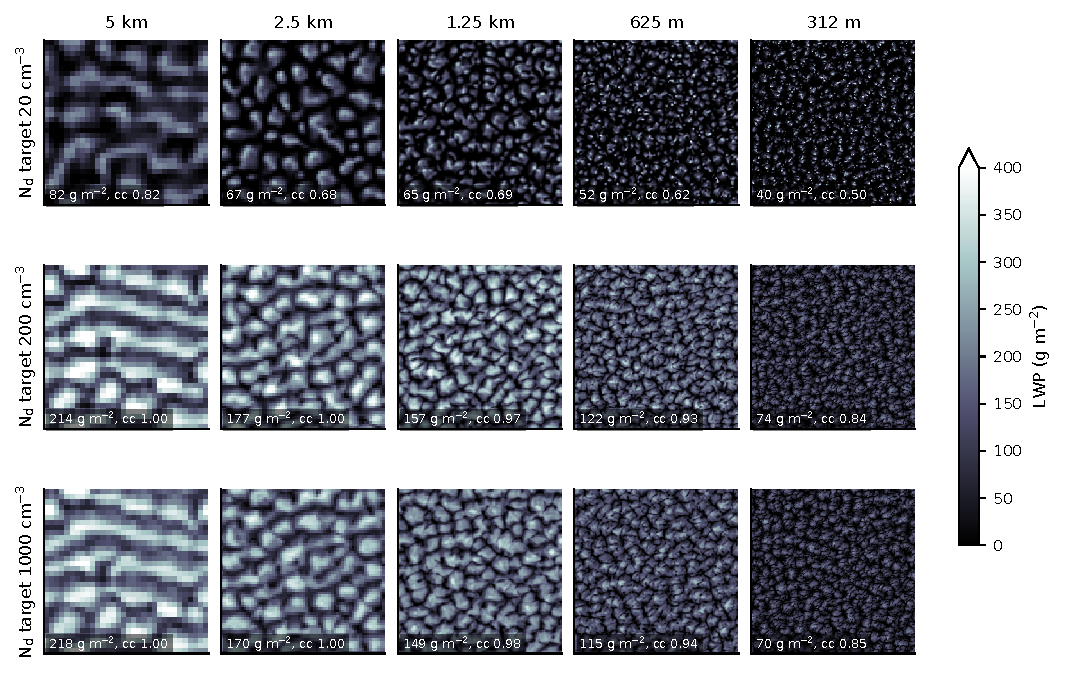
\includegraphics[width=\textwidth]{figures/fig01_maps.pdf}
\caption{Instantaneous LWP at hour 12 over the 240\,km domain for target $\Nd$ of 20, 200 and 1000\,$\cmthree$ (rows) and grid spacings from 5\,km to 312\,m (columns), for sedimentation factor 1 with $\Nd$-dependent autoconversion.}\label{fig:maps}
\end{figure}
\DIFaddend 

\DIFdelbegin %DIFDELCMD < \subsection{Cloud structure and mean state across grid spacings}\label{sec:morph}
%DIFDELCMD < %%%
\DIFdelend \DIFaddbegin \begin{figure}[t]
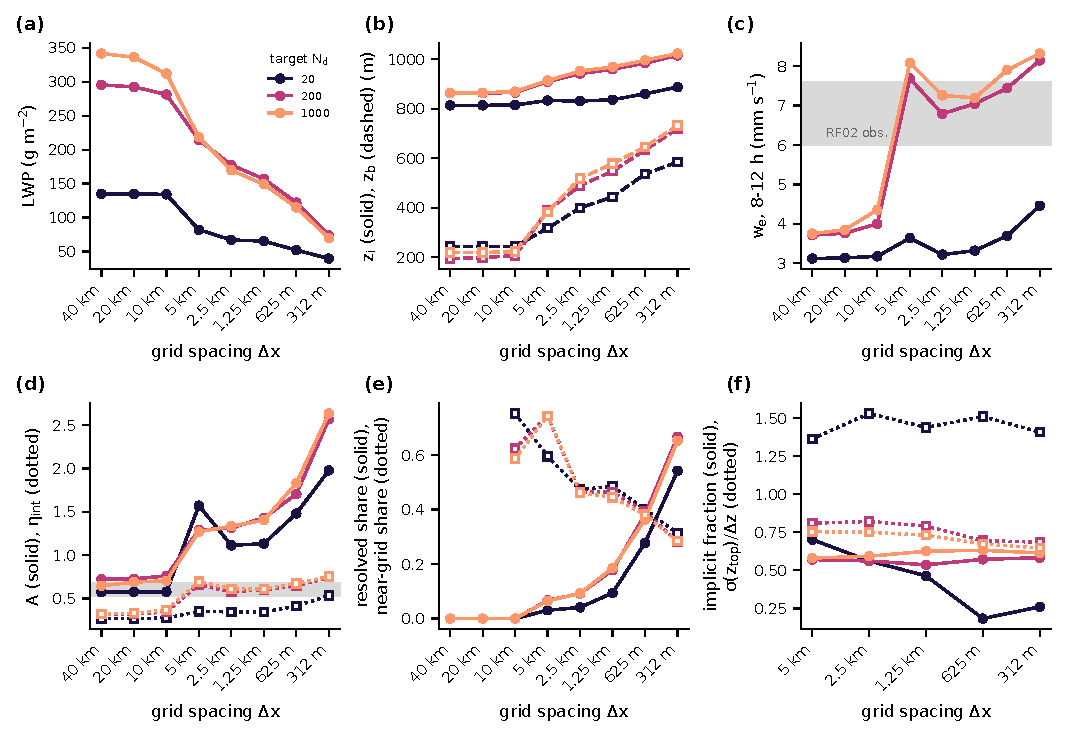
\includegraphics[width=\textwidth]{figures/fig02_meanstate.pdf}
\caption{Mean state against grid spacing for target $\Nd$ of 20, 200 and 1000\,$\cmthree$ (sedimentation factor 1, $\Nd$-dependent autoconversion, hours 10--12). (a) LWP. (b) Inversion height (solid) and cloud base (dashed). (c) Entrainment rate (8--12\,h fit) with the observed range. (d) Entrainment efficiency $A$ (solid) and $\eta$ with the specified interface jump (dotted), with the observed $\eta$ range. (e) Resolved share of boundary-layer vertical-velocity variance (solid) and share of resolved variance at wavelengths shorter than six physics-column spacings (dotted). (f) Fraction of the implied entrainment flux of $\theta_l$ not carried by resolved and SHOC fluxes (solid), and spread of column cloud-top height relative to the 50\,m level spacing (dotted), for $\dx\leq5$\,km.}\label{fig:meanstate}
\end{figure}
\DIFaddend 

\DIFdelbegin \DIFdel{Figure~\ref{fig:maps} shows LWP at hour 12 for $s=1$ with precipitation suppression on. As the grid is refined, the LWP spectral peak shortens from about 30\,km at 2.5\,km to 13--22\,km at 625 and }\DIFdelend \DIFaddbegin \DIFadd{The increase of $\we$ with decreasing grid spacing is not simply an increase of resolved turbulence. The total vertical-velocity variance at }\DIFaddend 312\,m \DIFdelbegin \DIFdel{, the domain-mean LWP decreases, and clear gaps appear. Interpolated to a diagnosed in-cloud $\Nd$ of 200}\DIFdelend \DIFaddbegin \DIFadd{(about 0.09}\DIFaddend \,\DIFdelbegin \DIFdel{$\cmthree$, LWP is 273}\DIFdelend \DIFaddbegin \DIFadd{m$^2$}\DIFaddend \,\DIFdelbegin \DIFdel{$\gmm$ }\DIFdelend \DIFaddbegin \DIFadd{s$^{-2}$) is a quarter of that }\DIFaddend at 40\,km, \DIFdelbegin \DIFdel{204}\DIFdelend \DIFaddbegin \DIFadd{the convective velocity scale is similar at all spacings (0.9--1.3}\DIFaddend \,\DIFdelbegin \DIFdel{$\gmm$ at 5}\DIFdelend \DIFaddbegin \DIFadd{m}\DIFaddend \,\DIFdelbegin \DIFdel{km and 73\,$\gmm$ at 312\,m}\DIFdelend \DIFaddbegin \DIFadd{s$^{-1}$)}\DIFaddend , and the \DIFdelbegin \DIFdel{maximum-overlap cloud cover decreases from 1.00 at $\dx\geq2.5$}\DIFdelend \DIFaddbegin \DIFadd{efficiency $A$ rises from 0.6--0.8 at $\dx\geq10$}\DIFaddend \,km to \DIFdelbegin \DIFdel{0.92 at }\DIFdelend \DIFaddbegin \DIFadd{1.1--1.6 at 5--1.25\,km, 1.5--1.8 at 625\,m and 2.0--2.6 at }\DIFaddend 312\,m \DIFdelbegin \DIFdel{. At target $\Nd=20\,\cmthree$ }\DIFdelend \DIFaddbegin \DIFadd{(Fig.~\ref{fig:meanstate}d). At $\dx\leq5$\,km and target $\Nd\geq200\,\cmthree$, }\DIFaddend the \DIFdelbegin \DIFdel{sub-kilometre clouds break into small cells of high LWP, and the maximum-overlap cloud cover at 312}\DIFdelend \DIFaddbegin \DIFadd{resolved plus SHOC turbulent $\theta_l$ flux at its minimum below the inversion carries only 37--46}\DIFaddend \,\DIFdelbegin \DIFdel{m is 0.68 (0.50 with the LWP threshold). The 5}\DIFdelend \DIFaddbegin \DIFadd{\% of the implied entrainment flux $-\we\Delta\theta_l$ (with the jump taken 50}\DIFaddend \,\DIFdelbegin \DIFdel{km fields contain stripe-like structures with a wavelength of about six physics columns, close to the effective resolution }\DIFdelend \DIFaddbegin \DIFadd{m above $\zi$), a fraction that does not change systematically with grid spacing (Fig.~\ref{fig:meanstate}f). The remainder, which includes radiative cooling within the entrainment zone and implicit mixing by the vertical remapping and advection }\DIFaddend of the dynamical core, \DIFdelbegin \DIFdel{which suggests that the circulations at this spacingare partly numerical. Between 40}\DIFdelend \DIFaddbegin \DIFadd{is therefore as large as the explicit flux at every spacing. At target $\Nd\geq200\,\cmthree$ the inversion is two to three levels thick (100--175}\DIFaddend \,\DIFdelbegin \DIFdel{km and 312\,m at target 200\,$\cmthree$, the inversion rises from 863 to 1016\,}\DIFdelend m\DIFdelbegin \DIFdel{, cloud base rises from 195 to 720}\DIFdelend \DIFaddbegin \DIFadd{) at all grid spacings, and the standard deviation of column cloud-top height at high $\Nd$ is 32--41}\DIFaddend \,\DIFdelbegin \DIFdel{m, the cloud layer thins from 668 to 296\,}\DIFdelend m, \DIFdelbegin \DIFdel{and the mixed layer becomes 1.8}\DIFdelend \DIFaddbegin \DIFadd{less than one level. The entrainment interface is thus not resolved vertically at any grid spacing, and SHOC's mixing length is at its cap of 312}\DIFaddend \,\DIFdelbegin \DIFdel{K warmer. The 40 and 20}\DIFdelend \DIFaddbegin \DIFadd{m nearly everywhere in the boundary layer at 312}\DIFaddend \,\DIFdelbegin \DIFdel{km runs are nearly indistinguishable. The 10\,km runs differ from them at high $\Nd$ (LWP }\DIFdelend \DIFaddbegin \DIFadd{m. Together with the positive vertical-velocity skewness at }\DIFaddend 312\DIFdelbegin \DIFdel{instead of 342}\DIFdelend \,\DIFdelbegin \DIFdel{$\gmm$ }\DIFdelend \DIFaddbegin \DIFadd{m (0.09--0.24 }\DIFaddend at target \DIFdelbegin \DIFdel{1000}\DIFdelend \DIFaddbegin \DIFadd{$\Nd\geq100\,\cmthree$), these diagnostics indicate that the 312}\DIFaddend \,\DIFdelbegin \DIFdel{$\cmthree$), where their column LWP standard deviation reaches up to 27\,$\gmm$ across configurations, compared with at most 5\,$\gmm$ at 20 and 40\,km. Resolved motions carry no measurable vertical-velocity variance at $\dx\geq10$\,km (Sect.~\ref{sec:grey}), so these runs approximate a single-column configuration of the model physics, with the 10\,km runs beginning to develop weak horizontal structure}\DIFdelend \DIFaddbegin \DIFadd{m runs are not an approximation to LES of RF02, which use spacings of a few metres near the inversion \mbox{%DIFAUXCMD
\citep{ackerman2009}}\hskip0pt%DIFAUXCMD
, and that part of the increase in $\we$ with refinement may be numerical. Vertical refinement at the inversion would be needed to separate the physical from the numerical part \mbox{%DIFAUXCMD
\citep{stevens1999res,bogenschutz2023rrm}}\hskip0pt%DIFAUXCMD
}\DIFaddend .

\DIFdelbegin %DIFDELCMD < \begin{figure}[t]
%DIFDELCMD < 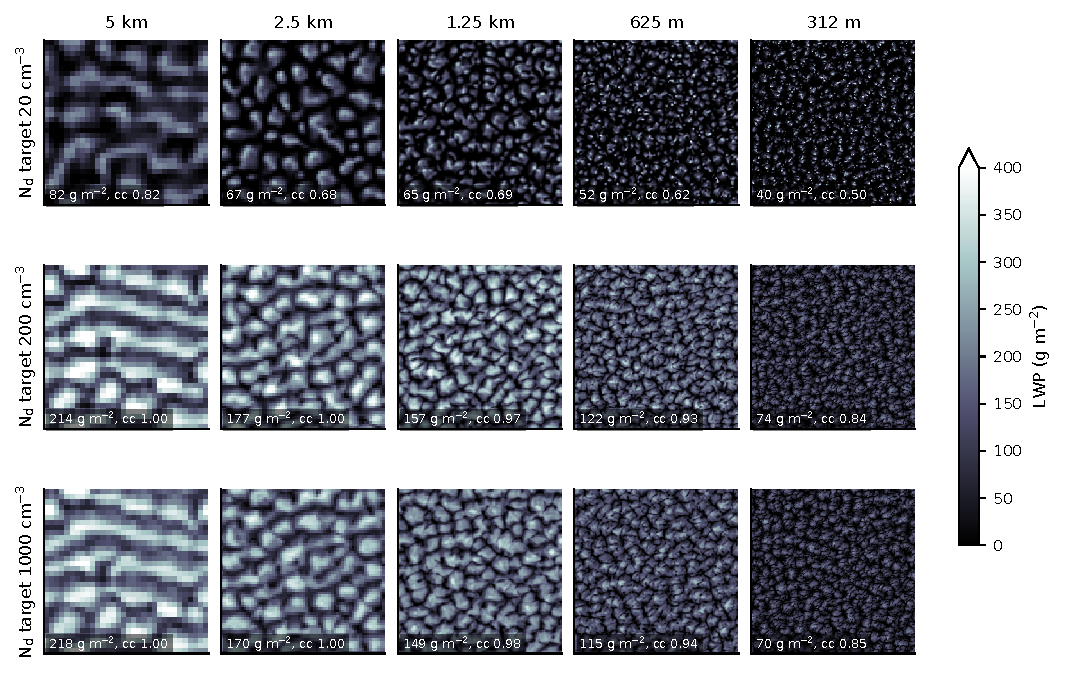
\includegraphics[width=\textwidth]{figures/fig01_maps.pdf}
%DIFDELCMD < \caption{Instantaneous LWP at hour 12 over the 240\,km domain for target $\Nd$ of 20, 200 and 1000\,$\cmthree$ (rows) and grid spacings from 5\,km to 312\,m (columns), for sedimentation factor 1 with precipitation suppression on and 3D turbulence off.}\label{fig:maps}
%DIFDELCMD < \end{figure}
%DIFDELCMD < 

%DIFDELCMD < \begin{table}[t]
%DIFDELCMD < \caption{Domain-mean LWP ($\gmm$, hours 10--12) for sedimentation factor 1 and 3D turbulence off, at the target $\Nd$ ($\cmthree$) of each column. Bold marks the maximum with precipitation suppression on. Diagnosed in-cloud $\Nd$ at a given target differs between grid spacings (Sect.~2.3).}\label{tab:lwp}
%DIFDELCMD < \begin{tabular}{llrrrrrr}
%DIFDELCMD < \tophline
%DIFDELCMD < $\dx$ & supp. & 20 & 50 & 100 & 200 & 500 & 1000 \\
%DIFDELCMD < \middlehline
%DIFDELCMD < 40\,km & on & 135 & 188 & 246 & 295 & 333 & \textbf{342} \\
 & off & 234 & 221 & 216 & 211 & 209 & 208 \\
\noalign{\vskip 2pt}
20\,km & on & 135 & 187 & 244 & 292 & 328 & \textbf{336} \\
 & off & 233 & 220 & 215 & 211 & 209 & 207 \\
\noalign{\vskip 2pt}
10\,km & on & 134 & 186 & 240 & 281 & 308 & \textbf{312} \\
 & off & 232 & 217 & 213 & 208 & 206 & 204 \\
\noalign{\vskip 2pt}
5\,km & on & 82 & 137 & 184 & 214 & \textbf{222} & 218 \\
 & off & 135 & 149 & 153 & 158 & 159 & 160 \\
\noalign{\vskip 2pt}
2.5\,km & on & 67 & 119 & 163 & \textbf{177} & 175 & 170 \\
 & off & 117 & 137 & 139 & 138 & 137 & 136 \\
\noalign{\vskip 2pt}
1.25\,km & on & 65 & 111 & 149 & \textbf{157} & 154 & 149 \\
 & off & 116 & 127 & 127 & 124 & 122 & 122 \\
\noalign{\vskip 2pt}
625\,m & on & 52 & 98 & 120 & \textbf{122} & 119 & 115 \\
 & off & 103 & 109 & 108 & 103 & 101 & 99 \\
\noalign{\vskip 2pt}
312\,m & on & 40 & 72 & \textbf{76} & 74 & 72 & 70 \\
 & off & 79 & 79 & 72 & 69 & 66 & 64 \\
\bottomhline

%DIFDELCMD < \end{tabular}
%DIFDELCMD < \end{table}
%DIFDELCMD < 

%DIFDELCMD < \subsection{LWP response to droplet number}\label{sec:response}
%DIFDELCMD < 

%DIFDELCMD < %%%
\DIFdel{Figure~\ref{fig:response} and Table~\ref{tab:lwp} show the LWP response to $\Nd$.With precipitation suppression on, LWP increases monotonically with $\Nd$ }\DIFdelend \DIFaddbegin \DIFadd{The efficiency $\eta$ illustrates how strongly the interpretation depends on the jump definition (Fig.~\ref{fig:entrain}c). With the jump taken 100\,m above $\zi$, $\eta$ is 0.6--0.7 }\DIFaddend at $\dx\geq10$\,km \DIFdelbegin \DIFdel{, from 135 to 342}\DIFdelend \DIFaddbegin \DIFadd{and 1.0--1.3 at finer spacing; with the specified interface jump of 6.7}\DIFaddend \,\DIFdelbegin \DIFdel{$\gmm$ at 40}\DIFdelend \DIFaddbegin \DIFadd{K it is 0.3--0.4 and 0.6--0.75, below the steady-state reference of 0.7--0.8. With the same definitions, the observed RF02 entrainment rate gives $\eta=0.9$--1.2 and 0.53--0.68. The coarse runs therefore entrain too little compared with RF02, and the sub-kilometre runs entrain at the upper end of the observed range; $\eta>1$ in the earlier definition reflected the 100}\DIFaddend \,\DIFdelbegin \DIFdel{km. With decreasing grid spacing, the curve flattens at high $\Nd$ and then turns over. The LWP maximum moves from target $\Nd\geq1000\,\cmthree$ at $\dx\geq10$\,km to 500\,$\cmthree$ at }\DIFdelend \DIFaddbegin \DIFadd{m offset, which adds about }\DIFaddend 5\,\DIFdelbegin \DIFdel{km, 200\,$\cmthree$ from 2.5\,km to 625\,m, and 100\,$\cmthree$ (diagnosed 84\,$\cmthree$) at 312\,m. The resulting shape resembles the inverted-V shape in satellite composites and LES ensembles \mbox{%DIFAUXCMD
\citep{gryspeerdt2019,glassmeier2021}}\hskip0pt%DIFAUXCMD
, but in these simulations it appears only at $\dx\leq5$\,km, and the negative slopes are an order of magnitude smaller than the observed ones, which \mbox{%DIFAUXCMD
\citet{gryspeerdt2019} }\hskip0pt%DIFAUXCMD
regarded as an upper bound on the causal effect}\DIFdelend \DIFaddbegin \DIFadd{K of the free-tropospheric $\theta_l$ profile}\DIFaddend .

\DIFdelbegin \DIFdel{With precipitation suppression off (Fig.~\ref{fig:response}b), LWP decreases slightly with $\Nd$ at $\dx\geq10$}\DIFdelend \DIFaddbegin \DIFadd{Table~\ref{tab:obs} compares hours 4--6 at target $\Nd=50\,\cmthree$ with the observations and the published simulations. The runs at $\dx\geq5$}\DIFaddend \,km \DIFdelbegin \DIFdel{(from 234 to 208}\DIFdelend \DIFaddbegin \DIFadd{resemble the DHARMA LES of \mbox{%DIFAUXCMD
\citet{wyant2007} }\hskip0pt%DIFAUXCMD
in LWP (156--159 compared with 144}\DIFaddend \,$\gmm$\DIFdelbegin \DIFdel{at 40}\DIFdelend \DIFaddbegin \DIFadd{) and entrainment (4.1 compared with 4.5}\DIFaddend \,\DIFdelbegin \DIFdel{km) and at 312}\DIFdelend \DIFaddbegin \DIFadd{mm}\DIFaddend \,\DIFdelbegin \DIFdel{m (from 79 to 64}\DIFdelend \DIFaddbegin \DIFadd{s$^{-1}$) but precipitate less than observed. The 625}\DIFaddend \,\DIFdelbegin \DIFdel{$\gmm$) . At 5}\DIFdelend \DIFaddbegin \DIFadd{m runs are closest to the observations, with an LWP of 119}\DIFaddend \,\DIFdelbegin \DIFdel{km it increases monotonically, from 135 to 160\,}\DIFdelend $\gmm$, \DIFdelbegin \DIFdel{and at 2.5}\DIFdelend \DIFaddbegin \DIFadd{an entrainment rate of 6.3}\DIFaddend \,\DIFdelbegin \DIFdel{km to 625}\DIFdelend \DIFaddbegin \DIFadd{mm}\DIFaddend \,\DIFdelbegin \DIFdel{m it increases between target 20 and 50}\DIFdelend \DIFaddbegin \DIFadd{s$^{-1}$, surface precipitation of 0.28}\DIFaddend \,\DIFdelbegin \DIFdel{$\cmthree$ ($\Slow=0.08$--0.20) and decreases slightly at higher $\Nd$. Surface precipitation (Fig.~\ref{fig:response}d)decreases steeply with $\Nd$ when suppression is on, and more steeply at finer spacing; at 312\,m it is 0.011\,}\DIFdelend mm\,d\DIFdelbegin \DIFdel{$^{-1}$ }\DIFdelend \DIFaddbegin \DIFadd{$^{-1}$ and an evaporated fraction of 0.73, although the evaporated fraction may be favoured by the assumption that rain fills the grid cell. No grid spacing matches all observed quantities, and by hours 10--12 the sub-kilometre runs have thinned further (LWP 70--120\,$\gmm$ }\DIFaddend at target \DIFdelbegin \DIFdel{100}\DIFdelend \DIFaddbegin \DIFadd{50--200}\DIFaddend \,\DIFdelbegin \DIFdel{$\cmthree$ and }\DIFdelend \DIFaddbegin \DIFadd{$\cmthree$).
}

\begin{table}[t]
\caption{Hours 4--6 at target $\Nd=50\,\cmthree$ and sedimentation factor 1, compared with RF02 observations and published simulations. $P_\mathrm{sfc}$ is surface precipitation and $f_\mathrm{evap}$ the fraction of rain production that evaporates before reaching the surface. Observations: LWP and $f_\mathrm{evap}$ as compiled by \citet{wyant2007}, $\we$ from \citet{faloona2005}, $P_\mathrm{sfc}$ from \citet{vanzanten2005}. The LES entry is the single DHARMA simulation and the SCM range covers nine models, both averaged over hours 4--6 from Table~2 of \citet{wyant2007} (standard vertical resolution).}\label{tab:obs}
\begin{tabular}{llrrrrrr}
\tophline
$\dx$ & autoconv. & LWP ($\gmm$) & $\we$ (mm\,s$^{-1}$) & $P_\mathrm{sfc}$ (mm\,d$^{-1}$) & $f_\mathrm{evap}$ & $\zb$ (m) & $\zi$ at 6\,h (m) \\
\middlehline
40\,km & on & 159 & 4.2 & 0.14 & 0.85 & 303 & 849 \\
20\,km & on & 158 & 4.1 & 0.13 & 0.85 & 303 & 849 \\
10\,km & on & 157 & 4.1 & 0.12 & 0.86 & 299 & 850 \\
5\,km & on & 156 & 4.1 & 0.13 & 0.85 & 303 & 851 \\
2.5\,km & on & 132 & 4.5 & 0.68 & 0.52 & 432 & 864 \\
1.25\,km & on & 132 & 5.1 & 0.52 & 0.61 & 443 & 870 \\
625\,m & on & 119 & 6.3 & 0.28 & 0.73 & 506 & 888 \\
312\,m & on & 98 & 7.7 & 0.10 & 0.84 & 578 & 913 \\
\noalign{\vskip 2pt}
40\,km & off & 171 & 4.2 & 0.05 & 0.91 & 303 & 851 \\
20\,km & off & 171 & 4.2 & 0.05 & 0.91 & 303 & 852 \\
10\,km & off & 170 & 4.2 & 0.05 & 0.92 & 313 & 852 \\
5\,km & off & 168 & 4.2 & 0.06 & 0.90 & 313 & 853 \\
2.5\,km & off & 141 & 4.5 & 0.52 & 0.55 & 432 & 866 \\
1.25\,km & off & 142 & 5.3 & 0.42 & 0.63 & 443 & 872 \\
625\,m & off & 125 & 6.8 & 0.23 & 0.73 & 501 & 891 \\
312\,m & off & 103 & 7.7 & 0.08 & 0.85 & 572 & 914 \\
\middlehline

Observations & & $100\pm20$ & 6.0--7.6 & 0.35 & 0.73 & & \\
DHARMA LES & & 144 & 4.5 & & & & \\
SCMs (9 models) & & 30--162 & 1.5--6.8 & & & & \\
\bottomhline
\end{tabular}
\end{table}

\subsection{Susceptibility after 10--12 h}\label{sec:susc}

\DIFadd{With $\Nd$-dependent autoconversion, LWP increases monotonically with $\Nd$ }\DIFaddend at \DIFdelbegin \DIFdel{most 0.002}\DIFdelend \DIFaddbegin \DIFadd{$\dx\geq10$}\DIFaddend \,\DIFdelbegin \DIFdel{mm\,d$^{-1}$ at higher }\DIFdelend \DIFaddbegin \DIFadd{km, whereas at finer spacing it flattens and then decreases slightly at high }\DIFaddend $\Nd$ \DIFdelbegin \DIFdel{. The entrainment rate }\DIFdelend (Fig.~\ref{fig:response}\DIFdelbegin \DIFdel{c)is 3.1--4.5\,mm\,s$^{-1}$ at $\dx\geq10$\,km and increases with }\DIFdelend \DIFaddbegin \DIFadd{). With }\DIFaddend $\Nd$\DIFdelbegin \DIFdel{at $\dx\leq5$\,km whether suppression is on or off. It is not monotonic in $\dx$: at target $\Nd\geq100\,\cmthree$ it is larger at 5\,km (7.0--8.1\,mm\,s$^{-1}$) than at 2.5\,km (5.7--7.3\,mm\,s$^{-1}$), and it increases again towards 312\,m (8.0--8.3\,mm\,s$^{-1}$). }%DIFDELCMD < 

%DIFDELCMD < \begin{figure}[t]
%DIFDELCMD < 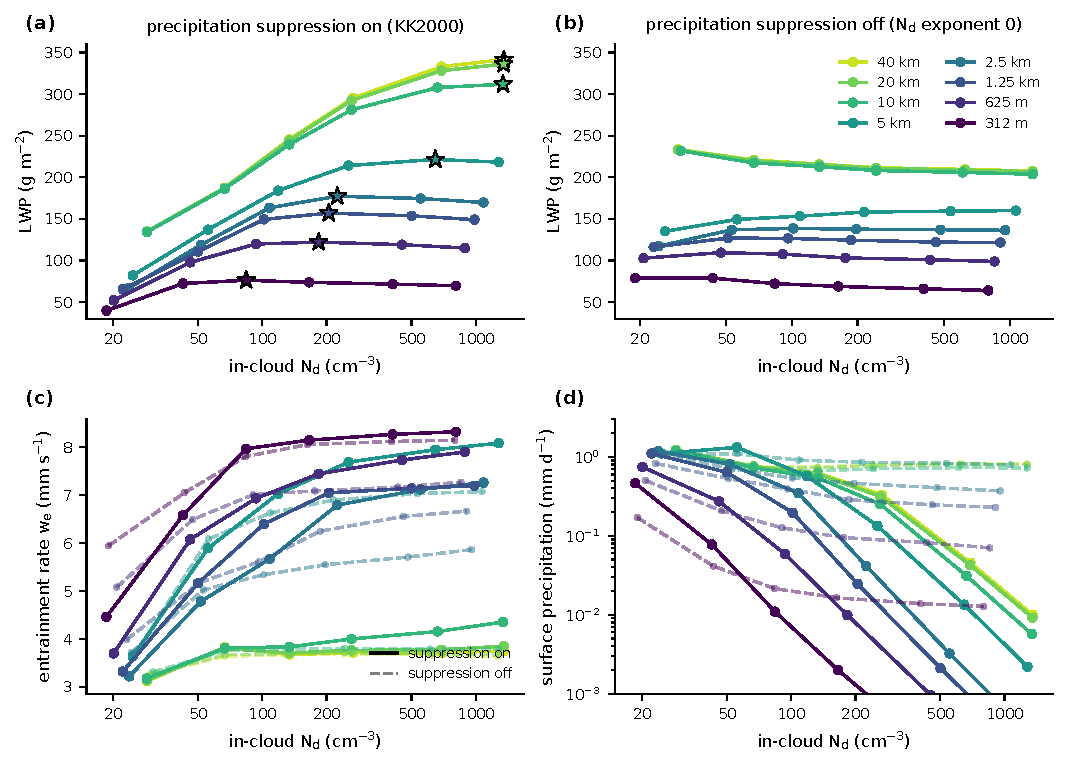
\includegraphics[width=\textwidth]{figures/fig02_response.pdf}
%DIFDELCMD < \caption{Response to $\Nd$ at every grid spacing (colours and symbols) for sedimentation factor 1. (a) LWP with precipitation suppression on; stars mark the maximum. (b) LWP with suppression off. (c) Entrainment rate (8--12\,h fit) and (d) surface precipitation, with suppression on (solid) and off (dashed); values below $10^{-4}$\,mm\,d$^{-1}$ are plotted at the lower axis limit. Values are hour 10--12 means against the diagnosed in-cloud $\Nd$.}\label{fig:response}
%DIFDELCMD < \end{figure}
%DIFDELCMD < 

%DIFDELCMD < %%%
\DIFdel{Figure~\ref{fig:susc} and }\DIFdelend \DIFaddbegin \DIFadd{-independent autoconversion it is nearly flat at all spacings. }\DIFaddend Table~\ref{tab:S} \DIFdelbegin \DIFdel{give the corresponding susceptibilities. With suppression on and $s=1$, }\DIFdelend \DIFaddbegin \DIFadd{and Fig.~\ref{fig:Scomp} give the susceptibilities. The moderate branch }\DIFaddend $\Shigh$ decreases \DIFdelbegin \DIFdel{monotonically as $\dx$ decreases, from 0.27 }\DIFdelend \DIFaddbegin \DIFadd{from 0.25 }\DIFaddend at 40\,km to \DIFdelbegin \DIFdel{0.20 }\DIFdelend \DIFaddbegin \DIFadd{0.21 }\DIFaddend at 5\,km, 0.11 at 2.5\,km, 0.07 at 1.25\,km, 0.03 at 625\,m and $-0.05$ at 312\,m\DIFaddbegin \DIFadd{, and it is entirely an in-cloud response}\DIFaddend . The polluted branch $\Svhigh$ changes sign between 5 \DIFdelbegin \DIFdel{\,km (0.01) }\DIFdelend and 2.5\,km \DIFdelbegin \DIFdel{($-0.03$) and lies between $-0.03$ }\DIFdelend and \DIFaddbegin \DIFadd{is $-0.03$ to }\DIFaddend $-0.04$ at finer spacing\DIFdelbegin \DIFdel{. }\DIFdelend \DIFaddbegin \DIFadd{; it is negative in 23 of the 24 configurations (sedimentation factor and autoconversion setting) at $\dx\leq2.5$\,km and becomes more negative with $s$ there ($-0.01$ to $-0.02$ for $s=0.5$ and $-0.06$ to $-0.09$ for $s=2$).
}

\DIFaddend The clean branch \DIFaddbegin \DIFadd{behaves differently. }\DIFaddend $\Slow$ increases from \DIFdelbegin \DIFdel{0.39 }\DIFdelend \DIFaddbegin \DIFadd{0.37 }\DIFaddend at $\dx\geq10$\,km to \DIFdelbegin \DIFdel{0.65}\DIFdelend \DIFaddbegin \DIFadd{0.62}\DIFaddend --0\DIFdelbegin \DIFdel{.76 at $\dx\leq2.5$}\DIFdelend \DIFaddbegin \DIFadd{.75 at $\dx\leq5$}\DIFaddend \,km\DIFdelbegin \DIFdel{. At sub-kilometre spacing, part of this increase is an increase in cloud cover; }\DIFdelend \DIFaddbegin \DIFadd{, and }\DIFaddend at 312\,m \DIFdelbegin \DIFdel{the cloud-cover }\DIFdelend \DIFaddbegin \DIFadd{0.32 of its 0.71 is cloud cover (0.52 with the LWP-threshold cover, which leaves an in-cloud }\DIFaddend part of \DIFdelbegin \DIFdel{$\Slow$ is 0.33 with the maximum-overlap definition (0.53 with the LWP threshold). On the high-}\DIFdelend \DIFaddbegin \DIFadd{0.19). At $\dx\geq10$\,km the cloud cover is 1.00 by both definitions, so a cloud-cover response is structurally absent there. The cloud-cover response also appears with }\DIFaddend $\Nd$\DIFdelbegin \DIFdel{branches cloud cover contributes less than 0.03. The temporal-sampling standard deviation is at most 0.03 at }\DIFdelend \DIFaddbegin \DIFadd{-independent autoconversion at }\DIFaddend $\dx\leq2.5$\,km\DIFdelbegin \DIFdel{and up to 0.1 }\DIFdelend \DIFaddbegin \DIFadd{, where cover increases with $\Nd$ while in-cloud LWP decreases, which points to droplet sedimentation or radiative effects on thin, broken cloud. Near the observed RF02 droplet number, the local susceptibility at a cloud-top $\Nd$ of 55\,$\cmthree$ is 0.35--0.47 from 40\,km to 1.25\,km, 0.29 }\DIFaddend at \DIFdelbegin \DIFdel{$\dx\geq5$}\DIFdelend \DIFaddbegin \DIFadd{625}\DIFaddend \,\DIFdelbegin \DIFdel{km, where LWP oscillates on time scales of about 15}\DIFdelend \DIFaddbegin \DIFadd{m and 0.06 at 312}\DIFaddend \,\DIFdelbegin \DIFdel{min. }%DIFDELCMD < 

%DIFDELCMD < %%%
\DIFdel{At }\DIFdelend \DIFaddbegin \DIFadd{m. A single fit of $\ln\LWP$ against $\ln\Nd$ over all six levels gives a positive slope at every spacing (0.22 at 40\,km and 0.10 at }\DIFaddend 312\,m\DIFdelbegin \DIFdel{, the negative $\Shigh$ corresponds to an LWP difference of 2.6}\DIFdelend \DIFaddbegin \DIFadd{), so the branch-wise values depend on the choice of branch boundaries, and the cloud-top $\Nd$ above which $|S|<0.1$ decreases from about 660}\DIFaddend \,\DIFdelbegin \DIFdel{$\gmm$ (3.4}\DIFdelend \DIFaddbegin \DIFadd{$\cmthree$ at 20--40}\DIFaddend \,\DIFdelbegin \DIFdel{\%) between targets }\DIFdelend \DIFaddbegin \DIFadd{km to 260\,$\cmthree$ at 2.5--10\,km, 110\,$\cmthree$ at 1.25\,km--625\,m and 54\,$\cmthree$ at 312\,m. The location of the LWP maximum is poorly constrained, because LWP at targets }\DIFaddend 100 and 200\,$\cmthree$ \DIFdelbegin \DIFdel{, and $\Svhigh$ to a difference of 4.1}\DIFdelend \DIFaddbegin \DIFadd{differs by only 3}\DIFaddend \,\DIFdelbegin \DIFdel{$\gmm$ between 200 and 1000\,$\cmthree$. These differences are smaller than the LWP decrease of each run in one hour (Sect.~\ref{sec:time}), and initial-condition spread in domain-mean LWP of stratocumulus simulations is typically of a few per cent. Without an ensemble, the sign of these small susceptibilities at }\DIFdelend \DIFaddbegin \DIFadd{\% at }\DIFaddend 312\,m \DIFdelbegin \DIFdel{is therefore not established.
The dependence on $s$ is more systematic. At $\dx\leq2.5$\,km with suppression on , $\Svhigh$ is $-0.01$ to $-0.02$ for $s=0.5$ }\DIFdelend and \DIFdelbegin \DIFdel{$-0.06$ to $-0.09$ for $s=2$ (Fig. ~\ref{fig:susc}c). }\DIFdelend \DIFaddbegin \DIFadd{625\,m.
}

\begin{figure}[t]
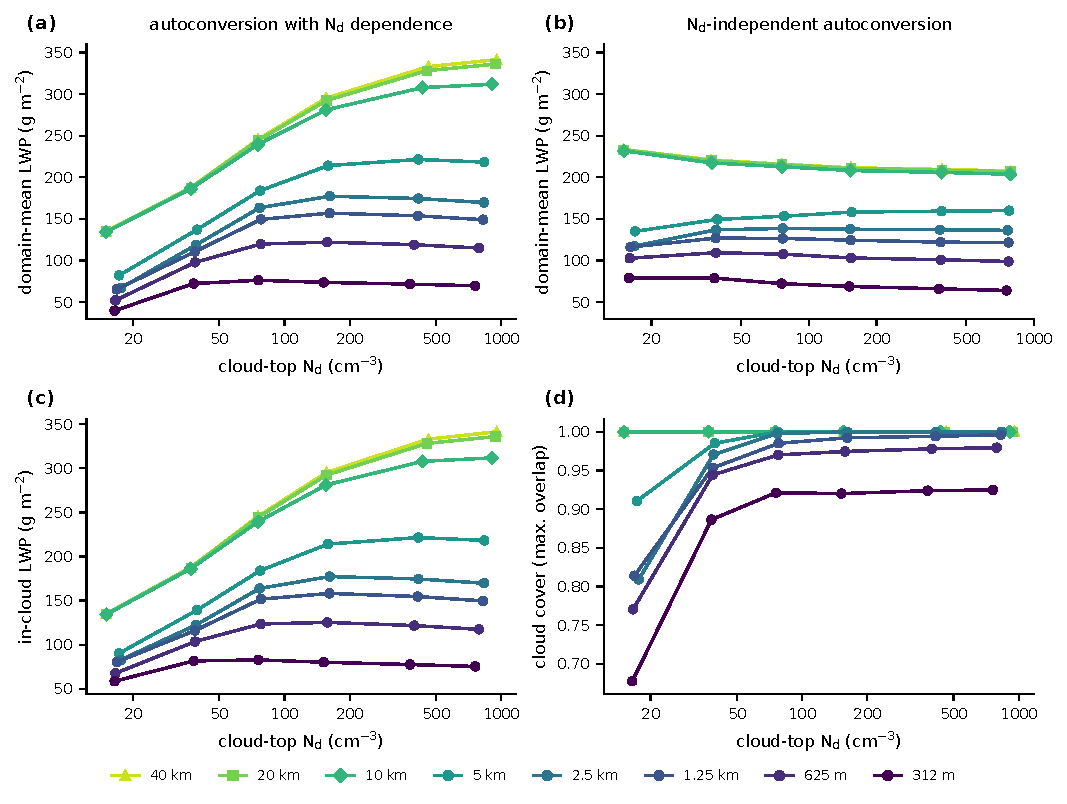
\includegraphics[width=\textwidth]{figures/fig03_response.pdf}
\caption{Response to cloud-top $\Nd$ at every grid spacing (sedimentation factor 1, hours 10--12). (a) Domain-mean LWP with $\Nd$-dependent and (b) $\Nd$-independent autoconversion. (c) In-cloud LWP and (d) maximum-overlap cloud cover with $\Nd$-dependent autoconversion.}\label{fig:response}
\end{figure}

\begin{figure}[t]
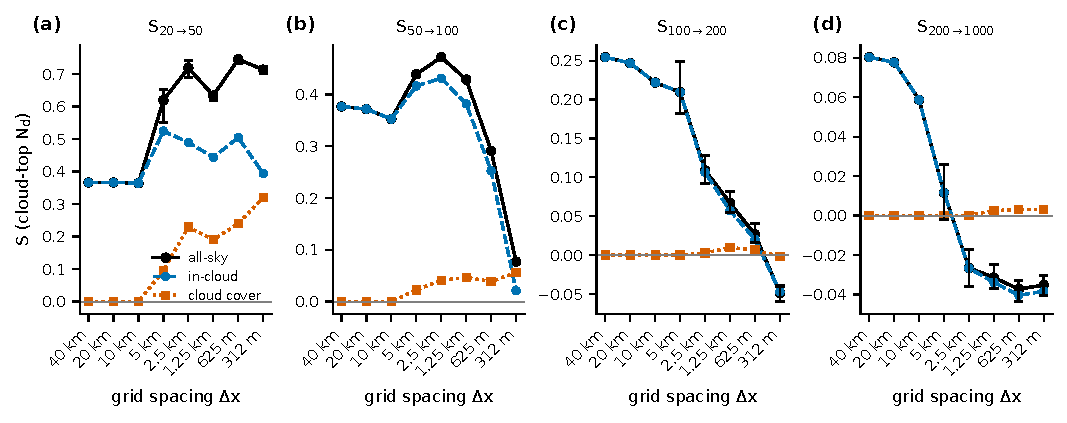
\includegraphics[width=\textwidth]{figures/fig04_Scomponents.pdf}
\caption{Susceptibility (cloud-top $\Nd$) on the four branches against grid spacing, split into in-cloud and cloud-cover parts (sedimentation factor 1, $\Nd$-dependent autoconversion, hours 10--12). Bars give the 5--95\,\% range of a 60\,km tile bootstrap ($\dx\leq5$\,km).}\label{fig:Scomp}
\end{figure}

\begin{table}[t]
\caption{Susceptibility with cloud-top $\Nd$ for sedimentation factor 1, hours 10--12. ``All'', ``ic'' and ``cc'' denote the all-sky value and its in-cloud and cloud-cover (maximum overlap) parts. ``Indep.'' denotes $\Nd$-independent autoconversion. $d\ln\tau/d\ln\Nd$ is for the moderate branch. $S_{55}$ is the local susceptibility at a cloud-top $\Nd$ of 55\,$\cmthree$ and $N_{0.1}$ the cloud-top $\Nd$ ($\cmthree$) above which $|S|<0.1$. Perturbed-twin and tile-bootstrap standard deviations are about 0.01 on the clean and moderate branches and 0.003 on the polluted branch at sub-kilometre spacing, and up to 0.03 at 5\,km.}\label{tab:S}
\begin{tabular}{lrrrrrrrrrrr}
\tophline
 & \multicolumn{3}{c}{$\Slow$} & \multicolumn{2}{c}{$\Shigh$} & $\Svhigh$ & \multicolumn{2}{c}{indep.} & & & \\
$\dx$ & all & ic & cc & all & ic & all & $\Shigh$ & $\Svhigh$ & $d\ln\tau/d\ln\Nd$ & $S_{55}$ & $N_{0.1}$ \\
\middlehline
40\,km & $0.37$ & $0.37$ & $0.00$ & $0.25$ & $0.25$ & $0.08$ & $-0.03$ & $-0.01$ & $0.55$ & 0.38 & 664 \\
20\,km & $0.37$ & $0.37$ & $0.00$ & $0.25$ & $0.25$ & $0.08$ & $-0.03$ & $-0.01$ & $0.54$ & 0.37 & 653 \\
10\,km & $0.36$ & $0.36$ & $0.00$ & $0.22$ & $0.22$ & $0.06$ & $-0.03$ & $-0.01$ & $0.52$ & 0.35 & 260 \\
5\,km & $0.62$ & $0.52$ & $0.10$ & $0.21$ & $0.21$ & $0.01$ & $0.05$ & $0.01$ & $0.51$ & 0.44 & 257 \\
2.5\,km & $0.72$ & $0.49$ & $0.23$ & $0.11$ & $0.11$ & $-0.03$ & $-0.01$ & $-0.01$ & $0.42$ & 0.47 & 259 \\
1.25\,km & $0.63$ & $0.44$ & $0.19$ & $0.07$ & $0.06$ & $-0.03$ & $-0.02$ & $-0.01$ & $0.38$ & 0.43 & 112 \\
625\,m & $0.75$ & $0.51$ & $0.24$ & $0.03$ & $0.02$ & $-0.04$ & $-0.06$ & $-0.03$ & $0.35$ & 0.29 & 111 \\
312\,m & $0.71$ & $0.39$ & $0.32$ & $-0.05$ & $-0.05$ & $-0.04$ & $-0.07$ & $-0.05$ & $0.29$ & 0.06 & 54 \\
\bottomhline

\end{tabular}
\end{table}

\DIFadd{The radiative meaning of these susceptibilities differs from their sign. The optical-depth susceptibility $d\ln\tau/d\ln\Nd$ stays positive on every branch at every spacing. }\DIFaddend On the moderate branch \DIFdelbegin \DIFdel{, $\Shigh$ increases with $s$ at 2.5 and 1.25}\DIFdelend \DIFaddbegin \DIFadd{it decreases from 0.55 at 40}\DIFaddend \,km \DIFdelbegin \DIFdel{(from 0.09 to 0.23 and from 0.06 }\DIFdelend to \DIFdelbegin \DIFdel{0.20) and decreases with $s$ }\DIFdelend \DIFaddbegin \DIFadd{0.29 }\DIFaddend at 312\,m\DIFdelbegin \DIFdel{(from $-0.02$ to $-0.08$). With suppression off, $S$ is within $\pm0.13$ of zero at $\dx\geq10$}\DIFdelend \DIFaddbegin \DIFadd{, and on the clean branch it is 0.64 at 40}\DIFaddend \,km \DIFdelbegin \DIFdel{on all branches. At $\dx\leq1.25$}\DIFdelend \DIFaddbegin \DIFadd{and 0.66--0.77 at finer spacing. In the offline albedo split, the LWP and cloud-cover terms amplify the Twomey term by 58}\DIFaddend \,\DIFdelbegin \DIFdel{km }\DIFdelend \DIFaddbegin \DIFadd{\% at 40\,km on the moderate branch and offset it by 13\,\% at 312\,m, while on the clean branch they amplify it by 91\,\% at 40\,km and by a factor of 2.0--3.2 at $\dx\leq5$\,km, mostly through cloud cover. On the polluted branch the adjustment changes from $+16\,\%$ to between $-5$ }\DIFaddend and \DIFdelbegin \DIFdel{$s\leq1$ it is negative on the two high-$\Nd$ branches ($-0.07$ and $-0.05$ at }\DIFdelend \DIFaddbegin \DIFadd{$-7\,\%$ of the Twomey term. The total potential albedo increase on the moderate branch is 0.079 at 40\,km and 0.046 at }\DIFaddend 312\,m\DIFdelbegin \DIFdel{for $s=1$)}\DIFdelend \DIFaddbegin \DIFadd{. A change in the sign of the LWP susceptibility at high $\Nd$ therefore reduces the implied brightening without reversing it, whereas the clean-branch increase at fine spacing amplifies it. Because clean regimes dominate the uncertainty in aerosol forcing \mbox{%DIFAUXCMD
\citep{carslaw2013} }\hskip0pt%DIFAUXCMD
and the cloud response to $\Nd$ is nonlinear \mbox{%DIFAUXCMD
\citep{jia2023}}\hskip0pt%DIFAUXCMD
, the clean-branch result is the more relevant one for forcing estimates}\DIFaddend .

\DIFdelbegin %DIFDELCMD < \begin{figure}[t]
%DIFDELCMD < 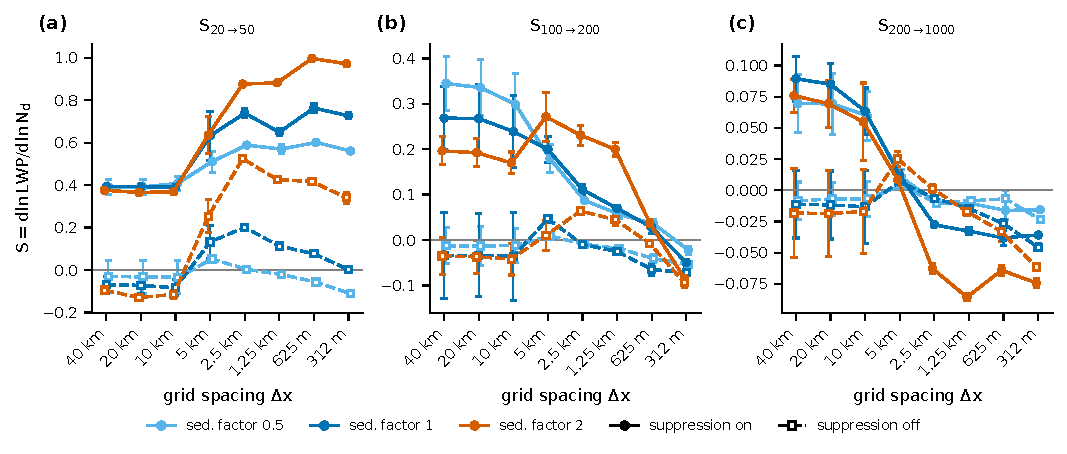
\includegraphics[width=\textwidth]{figures/fig03_susceptibility.pdf}
%DIFDELCMD < \caption{LWP susceptibility on the (a) clean, (b) moderate and (c) polluted branches against grid spacing (logarithmic axis). Colours: sedimentation factor. Solid lines and filled circles: precipitation suppression on; dashed lines and open squares: off. Bars show the standard deviation of $S$ over the eight 15\,min intervals in hours 10--12, a measure of temporal sampling only. Symbols are offset horizontally for clarity.}\label{fig:susc}
%DIFDELCMD < \end{figure}
%DIFDELCMD < 

%DIFDELCMD < \begin{table}[t]
%DIFDELCMD < \caption{Susceptibility $S=d\ln\LWP/d\ln\Nd$ for sedimentation factor 1 and 3D turbulence off. In parentheses: standard deviation over the eight 15\,min intervals in hours 10--12. The last column is the target $\Nd$ ($\cmthree$) of maximum LWP with suppression on.}\label{tab:S}
%DIFDELCMD < \begin{tabular}{lrrrrrrr}
%DIFDELCMD < \tophline
%DIFDELCMD <  & \multicolumn{2}{c}{$\Slow$} & \multicolumn{2}{c}{$\Shigh$} & \multicolumn{2}{c}{$\Svhigh$} & target $\Nd$ \\
%DIFDELCMD < $\dx$ & on & off & on & off & on & off & at max LWP \\
%DIFDELCMD < \middlehline
%DIFDELCMD < 40\,km & $0.393$\,(0.007) & $-0.070$\,(0.041) & $0.269$\,(0.070) & $-0.034$\,(0.095) & $0.089$\,(0.018) & $-0.011$\,(0.027) & 1000 \\
20\,km & $0.393$\,(0.006) & $-0.073$\,(0.039) & $0.267$\,(0.075) & $-0.034$\,(0.091) & $0.085$\,(0.017) & $-0.012$\,(0.027) & 1000 \\
10\,km & $0.390$\,(0.011) & $-0.084$\,(0.037) & $0.239$\,(0.079) & $-0.036$\,(0.097) & $0.063$\,(0.019) & $-0.013$\,(0.029) & 1000 \\
5\,km & $0.632$\,(0.117) & $0.132$\,(0.076) & $0.200$\,(0.029) & $0.047$\,(0.007) & $0.012$\,(0.004) & $0.007$\,(0.002) & 500 \\
2.5\,km & $0.740$\,(0.023) & $0.201$\,(0.010) & $0.111$\,(0.010) & $-0.010$\,(0.005) & $-0.028$\,(0.002) & $-0.006$\,(0.001) & 200 \\
1.25\,km & $0.650$\,(0.015) & $0.112$\,(0.004) & $0.070$\,(0.007) & $-0.025$\,(0.008) & $-0.033$\,(0.003) & $-0.015$\,(0.001) & 200 \\
625\,m & $0.764$\,(0.019) & $0.077$\,(0.003) & $0.028$\,(0.013) & $-0.065$\,(0.013) & $-0.038$\,(0.006) & $-0.027$\,(0.003) & 200 \\
312\,m & $0.727$\,(0.014) & $0.001$\,(0.013) & $-0.050$\,(0.008) & $-0.072$\,(0.006) & $-0.036$\,(0.001) & $-0.046$\,(0.003) & 100 \\
\bottomhline

%DIFDELCMD < \end{tabular}
%DIFDELCMD < \end{table}
%DIFDELCMD < 

%DIFDELCMD < \subsection{Temporal evolution of the susceptibility}%%%
\DIFdelend \DIFaddbegin \subsection{Temporal evolution}\DIFaddend \label{sec:time}

The \DIFdelbegin \DIFdel{susceptibilities evolve throughout the 12\,h }\DIFdelend \DIFaddbegin \DIFadd{resolution dependence develops during the simulations }\DIFaddend (Fig.~\ref{fig:time}). \DIFdelbegin \DIFdel{At $\dx\geq10$\,km, $\Shigh$ increases from 0.12 in }\DIFdelend \DIFaddbegin \DIFadd{In }\DIFaddend hours 2--4\DIFdelbegin \DIFdel{to 0.24}\DIFdelend \DIFaddbegin \DIFadd{, $\Shigh$ is 0.10}\DIFaddend --0\DIFdelbegin \DIFdel{.27 in hours 10--12, as the high-$\Nd$ clouds continue to gain the water that low-$\Nd$ clouds lose to precipitation (Fig.~\ref{fig:time}d); at }\DIFdelend \DIFaddbegin \DIFadd{.11 at every spacing from }\DIFaddend 40 \DIFaddbegin \DIFadd{to 2.5}\DIFaddend \,km and \DIFdelbegin \DIFdel{high $\Nd$, LWP is still increasing by up to 15}\DIFdelend \DIFaddbegin \DIFadd{close to zero at $\dx\leq1.25$}\DIFaddend \,\DIFdelbegin \DIFdel{$\gmm$\,h$^{-1}$ in }\DIFdelend \DIFaddbegin \DIFadd{km; by }\DIFaddend hours 10--12 \DIFdelbegin \DIFdel{. At 1.25}\DIFdelend \DIFaddbegin \DIFadd{it has grown to 0.21--0.25 at 5--40}\DIFaddend \,km and \DIFdelbegin \DIFdel{625}\DIFdelend \DIFaddbegin \DIFadd{has become negative at 312}\DIFaddend \,m, \DIFdelbegin \DIFdel{$\Shigh$ also increases slowly (from 0.00 to 0.07 and 0.03), whereas at 312}\DIFdelend \DIFaddbegin \DIFadd{while at 1.25}\DIFaddend \,\DIFdelbegin \DIFdel{m it decreases from 0.00 to $-0.05$}\DIFdelend \DIFaddbegin \DIFadd{km and 625\,m it has increased slightly}\DIFaddend . The polluted branch \DIFdelbegin \DIFdel{$\Svhigh$ becomes more negative with time at all $\dx\leq2.5$}\DIFdelend \DIFaddbegin \DIFadd{is 0.04 at $\dx\geq2.5$}\DIFaddend \,km \DIFdelbegin \DIFdel{, from about }\DIFdelend \DIFaddbegin \DIFadd{and }\DIFaddend $-0.01$ \DIFaddbegin \DIFadd{at finer spacing }\DIFaddend in hours 2--4\DIFaddbegin \DIFadd{, and it diverges in the same way. At 40\,km $S$ oscillates with periods of about 1.5--2\,h, so 2\,h averages are needed. The cloud-top $\Nd$ of the LWP maximum falls below the highest $\Nd$ level after about 3\,h }\DIFaddend at $\dx\leq1.25$\,km\DIFdelbegin \DIFdel{and from 0.04 }\DIFdelend \DIFaddbegin \DIFadd{, after 5\,h }\DIFaddend at 2.5\,km \DIFdelbegin \DIFdel{to between $-0.03$ and $-0.04$ in hours 10--12. The clean branch is already large in hours 2--4 at 625 and }\DIFdelend \DIFaddbegin \DIFadd{and after about 9\,h at 5\,km, and at }\DIFaddend 312\,\DIFdelbegin \DIFdel{m (0.56--0.63) and at 1.25}\DIFdelend \DIFaddbegin \DIFadd{m it continues to decrease, from about 200 to 80}\DIFaddend \,\DIFdelbegin \DIFdel{km (0.51) and increases slowly. At $\dx\leq2.5$}\DIFdelend \DIFaddbegin \DIFadd{$\cmthree$ between 5 and 12}\DIFaddend \,\DIFaddbegin \DIFadd{h. The inverted-V shape is thus time-dependent, and the statement that the maximum lies near 100\,$\cmthree$ at 312\,m refers to hour 12.
}

\DIFadd{At $\dx\leq1.25$\,}\DIFaddend km, LWP decreases in \DIFdelbegin \DIFdel{98\,\% of the runs during hours 10--12, }\DIFdelend \DIFaddbegin \DIFadd{nearly all runs throughout hours 4--12, and the coarse runs at high $\Nd$ are still thickening (}\DIFaddend by up to \DIFdelbegin \DIFdel{4.4}\DIFdelend \DIFaddbegin \DIFadd{15}\DIFaddend \,$\gmm$\,h$^{-1}$ \DIFdelbegin \DIFdel{or 6}\DIFdelend \DIFaddbegin \DIFadd{at 40}\DIFaddend \,\DIFdelbegin \DIFdel{\%\,h$^{-1}$, and none of the susceptibilities at sub-kilometre spacing had levelled off at 12\,h. The adjustment time scales in these runs are therefore longer than the simulation}\DIFdelend \DIFaddbegin \DIFadd{km)}\DIFaddend , as in \DIFdelbegin \DIFdel{LES of non-precipitating stratocumulus, where LWP continues to adjust over a day or more \mbox{%DIFAUXCMD
\citep{glassmeier2021}}\hskip0pt%DIFAUXCMD
.}%DIFDELCMD < 

%DIFDELCMD < \begin{figure}[t]
%DIFDELCMD < 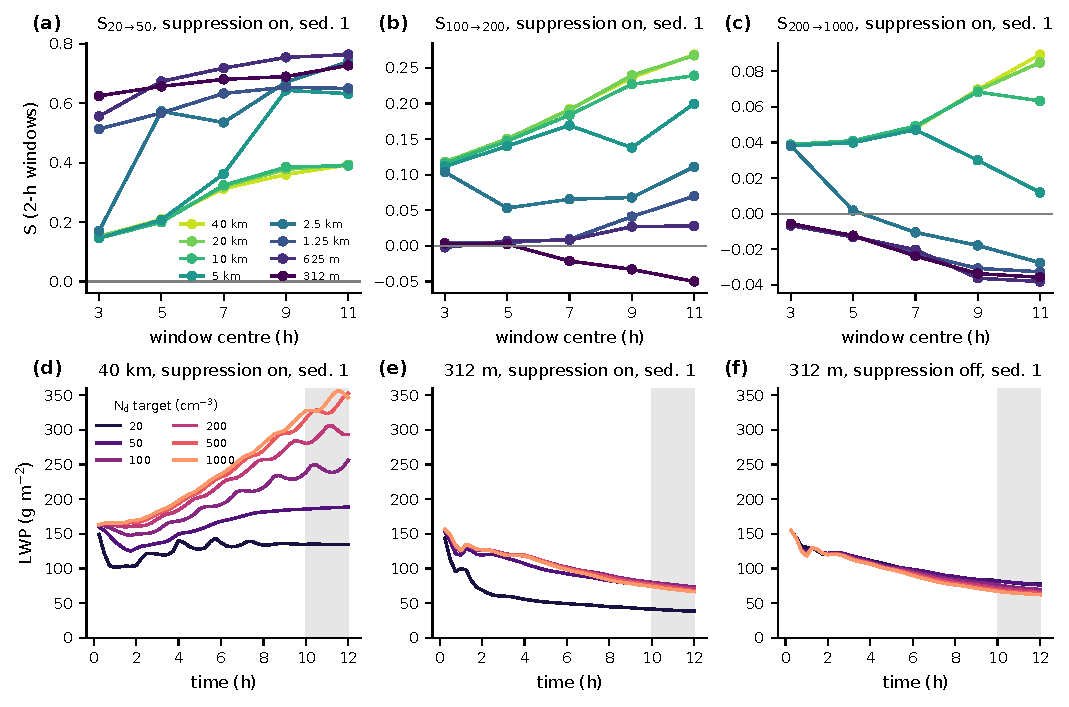
\includegraphics[width=\textwidth]{figures/fig04_time.pdf}
%DIFDELCMD < \caption{(a--c) Susceptibility on the three branches for consecutive 2\,h windows (suppression on, sedimentation factor 1), coloured by grid spacing. (d--f) LWP time series for each target $\Nd$ at 40\,km with suppression on and at 312\,m with suppression on and off. Grey shading marks the analysis window.}\label{fig:time}
%DIFDELCMD < \end{figure}
%DIFDELCMD < 

%DIFDELCMD < \subsection{Precipitation suppression, sedimentation and their interaction}\label{sec:attr}
%DIFDELCMD < 

%DIFDELCMD < %%%
\DIFdel{Figure~\ref{fig:decomp} shows the decomposition of Eq. ~(\ref{eq:decomp}) at $s=1$. At $\dx\geq10$\,km, the precipitation-suppression term at zero sedimentation is 0.34--0.39 on the moderate branch and 0.07--0.08 on the polluted branch, and the sedimentation term derived from the off runs is small ($-0.02$ to $-0.01$). The interaction term on the moderate branch is $-0.07$ to $-0.08$, because $\Shigh$ with suppression on decreases strongly with $s$ (from 0.35 to 0.20 between $s=0.5$ and 2 }\DIFdelend \DIFaddbegin \DIFadd{transient simulations of precipitating shallow convection \mbox{%DIFAUXCMD
\citep{seifert2015}}\hskip0pt%DIFAUXCMD
. The phase plane of $d\LWP/dt$ against LWP }\DIFaddend at \DIFdelbegin \DIFdel{40\,km), whereas the off runs barely respond. This sensitivity to sedimentation at coarse spacing is larger than at }\DIFdelend 312\,\DIFdelbegin \DIFdel{m ($dS_\mathrm{on}/ds=-0.10$ at 40\,km and $-0.04$ at }\DIFdelend \DIFaddbegin \DIFadd{m (Fig.~\ref{fig:time}d) shows a common decline for all $\Nd$ that slows towards the end of the run. Exponential relaxation fits over hours 6--12 are well constrained only at }\DIFaddend 312\,\DIFdelbegin \DIFdel{m). It is unlikely to act through entrainment, which changes by less than 0.6}\DIFdelend \DIFaddbegin \DIFadd{m, where they give time scales of 4--7}\DIFaddend \,\DIFdelbegin \DIFdel{mm}\DIFdelend \DIFaddbegin \DIFadd{h and equilibrium LWP of about 45--55}\DIFaddend \,\DIFdelbegin \DIFdel{s$^{-1}$ between $s=0.5$ and 2 at $\dx\geq10$}\DIFdelend \DIFaddbegin \DIFadd{$\gmm$ for $\Nd\geq50\,\cmthree$, 25--35}\DIFaddend \,\DIFdelbegin \DIFdel{km (Fig.~\ref{fig:entrain}a ). Deposition of cloud droplets at the surface is also unlikely to explain it, because the estimated deposition at the lowest model level exceeds 0.02}\DIFdelend \DIFaddbegin \DIFadd{\% below the 12}\DIFaddend \,\DIFdelbegin \DIFdel{mm}\DIFdelend \DIFaddbegin \DIFadd{h values. At coarser spacing the fits do not constrain an equilibrium within 24}\DIFaddend \,\DIFdelbegin \DIFdel{d$^{-1}$ only at $\dx\geq10$}\DIFdelend \DIFaddbegin \DIFadd{h. The steady-state susceptibility at 312}\DIFaddend \,\DIFdelbegin \DIFdel{km, target 20}\DIFdelend \DIFaddbegin \DIFadd{m implied by these fits, with 5--95}\DIFaddend \,\DIFdelbegin \DIFdel{$\cmthree$, $s=2$ with suppression off (up to 0.25}\DIFdelend \DIFaddbegin \DIFadd{\% intervals from a paired moving-block bootstrap, is $-0.11$ to $-0.21$ on the moderate branch in five of the six combinations of sedimentation and autoconversion setting (for $s=1$ and $\Nd$-dependent autoconversion $-0.13$, with an interval of $-0.23$ to $+0.06$), and $-0.17$ to $+0.06$ on the polluted branch. The negative moderate branch at 312}\DIFaddend \,\DIFdelbegin \DIFdel{mm}\DIFdelend \DIFaddbegin \DIFadd{m is therefore more likely to strengthen than to vanish as the runs approach equilibrium, while the sign of the polluted branch at equilibrium is undetermined. Fast and slow time scales coexist, as in mixed-layer and LES analyses \mbox{%DIFAUXCMD
\citep{bretherton2010,jones2014}}\hskip0pt%DIFAUXCMD
, and the inversion is far from its equilibrium. With a subsidence time scale of 74}\DIFaddend \,\DIFdelbegin \DIFdel{d$^{-1}$, or about 20}\DIFdelend \DIFaddbegin \DIFadd{h, $\we/D$ is about 1000}\DIFaddend \,\DIFdelbegin \DIFdel{\% of surface precipitation). The sensitivity to sedimentation at coarse spacing therefore depends on the autoconversion formulation, presumably through the vertical redistribution of cloud water relative to where rain forms, but we have not isolated its mechanism. In addition, because of the pivot dependence described in Sect.~\ref{sec:decomp}, the statement that precipitation suppression accounts for the positive response at coarse spacing holds for this design and should not be read as a pivot-independent attribution. }%DIFDELCMD < 

%DIFDELCMD < %%%
\DIFdel{At finer spacing, the precipitation-suppression term on the moderate branch decreases to 0.12 at 5}\DIFdelend \DIFaddbegin \DIFadd{m at 40}\DIFaddend \,km \DIFdelbegin \DIFdel{, 0.05--0.10 between 2.5}\DIFdelend \DIFaddbegin \DIFadd{and about 2200}\DIFaddend \,\DIFdelbegin \DIFdel{km and 625\,}\DIFdelend m \DIFdelbegin \DIFdel{and 0.04 }\DIFdelend at 312\,m, \DIFdelbegin \DIFdel{and on the polluted branch it is 0.00--0.02 at $\dx\leq5$}\DIFdelend \DIFaddbegin \DIFadd{compared with $\zi$ of 860 and 1020}\DIFaddend \,\DIFdelbegin \DIFdel{km. On the polluted branch at 2.5 and 1.25}\DIFdelend \DIFaddbegin \DIFadd{m at 12}\DIFaddend \,\DIFdelbegin \DIFdel{km, the negative $\Svhigh$ comes mainly from the interaction term ($-0.04$ and }\DIFdelend \DIFaddbegin \DIFadd{h. A susceptibility of about }\DIFaddend $-0.05$ \DIFdelbegin \DIFdel{) and the residual ($-0.01$), while the sedimentation term derived from the off runs is near zero ($+0.01$ and $-0.01$). At 625}\DIFdelend \DIFaddbegin \DIFadd{after 11}\DIFaddend \,\DIFdelbegin \DIFdel{m and 312}\DIFdelend \DIFaddbegin \DIFadd{h is weaker than the LWP adjustments found after a similar time in an LES ensemble of non-precipitating nocturnal stratocumulus \mbox{%DIFAUXCMD
\citep{chen2025}}\hskip0pt%DIFAUXCMD
.
}

\begin{figure}[t]
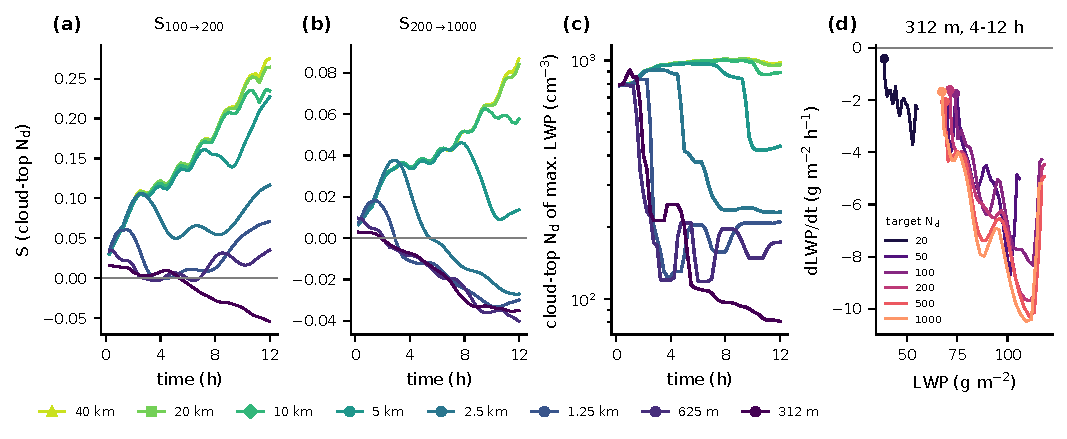
\includegraphics[width=\textwidth]{figures/fig05_time.pdf}
\caption{Temporal evolution ($\Nd$-dependent autoconversion, sedimentation factor 1). (a) $\Shigh$ and (b) $\Svhigh$ from 15\,min output (2\,h running mean). (c) Cloud-top $\Nd$ of the LWP maximum (2\,h running median); values near the top of the axis indicate a maximum at the highest $\Nd$ level. (d) Phase plane of $d\LWP/dt$ against LWP at 312\,m for hours 4--12; dots mark hour 12.}\label{fig:time}
\end{figure}

\subsection{Susceptibility and the base-state regime}\label{sec:regime}

\DIFadd{Figure~\ref{fig:regime} plots $S$ against the precipitation-to-entrainment-drying ratio of the lower-$\Nd$ run for all grid spacings, sedimentation factors and both autoconversion settings. With $\Nd$-dependent autoconversion, $\Shigh$ follows this ratio closely across the 24 combinations of grid spacing and sedimentation factor (correlation 0.92). The ratio alone explains 84}\DIFaddend \,\DIFdelbegin \DIFdel{m the sedimentation term ($-0.016$ and $-0.024$), the interaction ($-0.015$ at both) and the residual ($-0.004$ and $-0.016$)all contribute. On this branch, a larger sedimentation factor increases LWP more at target 200 than at 1000}\DIFdelend \DIFaddbegin \DIFadd{\% of the variance of $\Shigh$, and adding $\log\dx$ as a second predictor raises this only to 86}\DIFaddend \,\DIFdelbegin \DIFdel{$\cmthree$, so $\Svhigh$ becomes more negative }\DIFdelend \DIFaddbegin \DIFadd{\%. This also explains why $\Shigh$ increases }\DIFaddend with $s$ \DIFdelbegin \DIFdel{, consistent with the mechanism of \mbox{%DIFAUXCMD
\citet{bretherton2007}}\hskip0pt%DIFAUXCMD
. At }\DIFdelend \DIFaddbegin \DIFadd{at }\DIFaddend 2.5 and 1.25\,km\DIFdelbegin \DIFdel{the moderate branch behaves differently, with positive sedimentation and interaction terms (both about 0.05), so that $\Shigh$ increases with $s$. }%DIFDELCMD < 

%DIFDELCMD < %%%
\DIFdel{On the clean branch at $\dx\leq5$}\DIFdelend \DIFaddbegin \DIFadd{, because faster sedimentation raises the base-state surface precipitation there and moves the runs along the same curve. On the middle branch the correlation is 0.70, and on the polluted branch 0.75, where grid spacing retains additional explanatory power (variance explained 57}\DIFaddend \,\DIFdelbegin \DIFdel{km, the sedimentation term is positive (0.13 at 5}\DIFdelend \DIFaddbegin \DIFadd{\% by the ratio alone and 85}\DIFaddend \,\DIFdelbegin \DIFdel{km and 0.30--0.34 at $\dx\leq2.5$\,km). At target $\Nd=20\,\cmthree$, cloud-top effective radii are 12--14\,$\mu$m for $s=1$ with suppression on, and a larger sedimentation factor lowers LWP most at the lowest $\Nd$. At these droplet sizes, sedimentation mainly removes cloud water, as drizzle does, and its effect on entrainment is secondary. The clean-branch residual is large and negative at $\dx\leq2.5$\,km ($-0.16$ to $-0.28$) , but it is the least well constrained term because $S_\mathrm{off}$ is convex in $s$ ($-0.11$}\DIFdelend \DIFaddbegin \DIFadd{\% with $\log\dx$)}\DIFaddend , \DIFdelbegin \DIFdel{0.00 }\DIFdelend \DIFaddbegin \DIFadd{consistent with the change in entrainment efficiency at constant, nearly zero precipitation. With $\Nd$-independent autoconversion the relationship is weaker (correlations 0.45--0.65) }\DIFaddend and \DIFdelbegin \DIFdel{0.34 for $s=0.5$, 1 and 2 at 312\,m).
We interpret it only as an indication that pathways other than a linear sedimentation effect, possibly including radiative effective-radius effects on thin, broken clouds, contribute on this branch.
}\DIFdelend \DIFaddbegin \DIFadd{$S$ is near zero over most of the range. On the clean branch the ratio has no explanatory power, because the response there is dominated by cloud cover at fine spacing.
}\DIFaddend 

\DIFdelbegin %DIFDELCMD < \begin{figure}[t]
%DIFDELCMD < 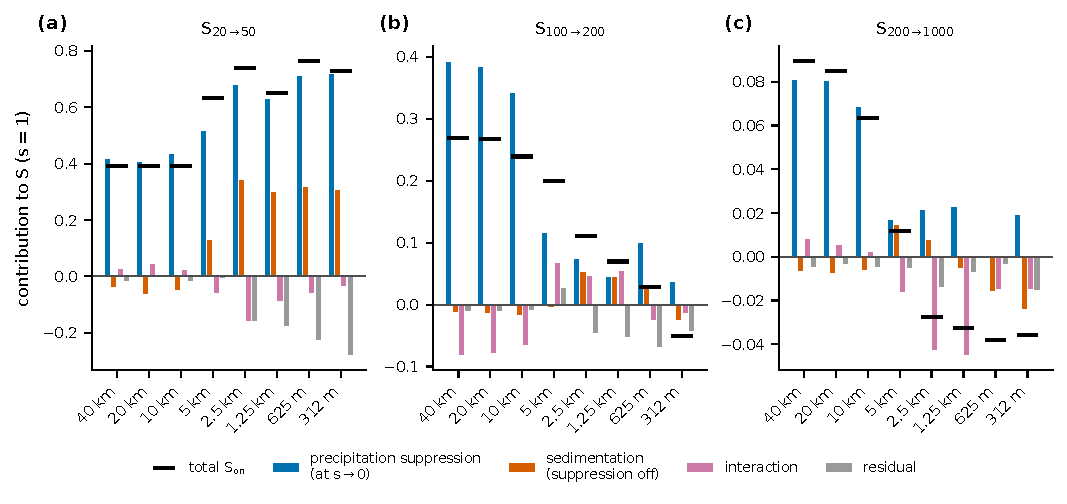
\includegraphics[width=\textwidth]{figures/fig05_decomposition.pdf}
%DIFDELCMD < \caption{Decomposition (Eq.~\ref{eq:decomp}) of the susceptibility with suppression on at sedimentation factor 1 (black bars) on the (a) clean, (b) moderate and (c) polluted branches. Blue: precipitation suppression extrapolated to zero sedimentation; orange: sedimentation without precipitation suppression; pink: interaction; grey: residual. The partition at coarse spacing depends on the matching $\Nd$ of the suppression-off configuration (Sect.~\ref{sec:decomp}).}\label{fig:decomp}
%DIFDELCMD < \end{figure}
%DIFDELCMD < %%%
\DIFdelend \DIFaddbegin \begin{figure}[t]
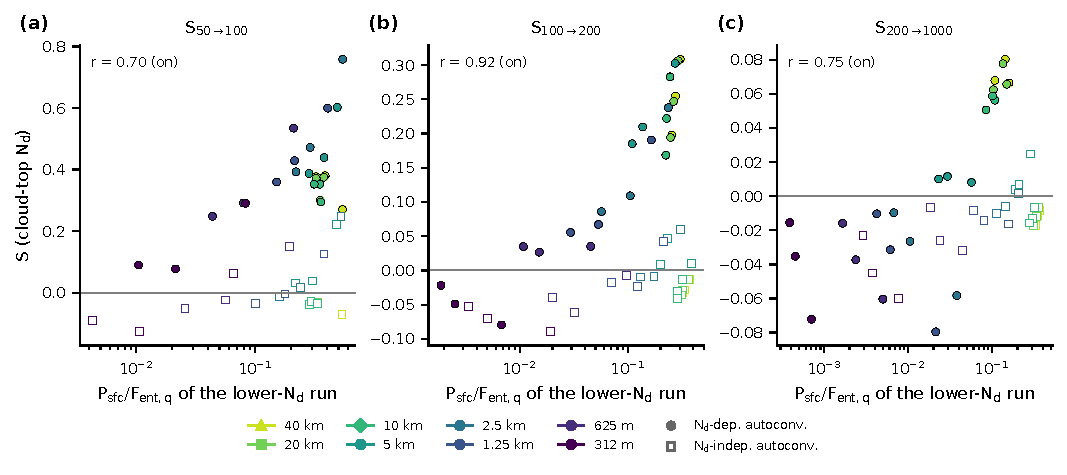
\includegraphics[width=\textwidth]{figures/fig06_regime.pdf}
\caption{Susceptibility (cloud-top $\Nd$, hours 10--12) against the ratio of surface precipitation to entrainment drying of the lower-$\Nd$ run, for all grid spacings and sedimentation factors, on the (a) middle, (b) moderate and (c) polluted branches. Filled circles: $\Nd$-dependent autoconversion; open squares: $\Nd$-independent. Correlations refer to $\Nd$-dependent autoconversion.}\label{fig:regime}
\end{figure}
\DIFaddend 

\DIFdelbegin %DIFDELCMD < \subsection{Resolution dependence of the precipitation sink}\label{sec:rain}
%DIFDELCMD < 

%DIFDELCMD < %%%
\DIFdel{The effect of precipitation suppression on LWP is limited by the size of the precipitation sink, and Fig. ~\ref{fig:rain} shows that this sink decreases with grid spacing. Rain production (autoconversion plus accretion) }\DIFdelend \DIFaddbegin \DIFadd{The base state changes with grid spacing because the coarse and fine clouds differ in depth, base height and turbulence. Rain production }\DIFaddend at target 200\,$\cmthree$ decreases from 0.55\,mm\,d$^{-1}$ at 40\,km to 0.03\,mm\,d$^{-1}$ at 312\,m \DIFdelbegin \DIFdel{(Fig.~\ref{fig:rain}a), }\DIFdelend as the cloud thins from about 650 to \DIFdelbegin \DIFdel{about }\DIFdelend 300\,m\DIFdelbegin \DIFdel{(Fig.~\ref{fig:rain}d) and the KK2000 rates decrease steeply with cloud water. At target 20\,$\cmthree$ the decrease is smaller, from about 2.0 to 1.2\,mm\,d$^{-1}$. As cloud base rises, the fraction of rain production }\DIFdelend \DIFaddbegin \DIFadd{, and the fraction }\DIFaddend that evaporates below cloud \DIFdelbegin \DIFdel{increases, at target 200\,$\cmthree$ }\DIFdelend \DIFaddbegin \DIFadd{base increases }\DIFaddend from 0.40 \DIFdelbegin \DIFdel{at 40\,km }\DIFdelend to 0.93 \DIFdelbegin \DIFdel{at 312\,m }\DIFdelend (Fig.~\ref{fig:rain}\DIFdelbegin \DIFdel{b), consistent with the importance of subcloud evaporation in drizzling stratocumulus \mbox{%DIFAUXCMD
\citep{wood2005,wyant2007}}\hskip0pt%DIFAUXCMD
. At the same time the }\DIFdelend \DIFaddbegin \DIFadd{). Meanwhile the }\DIFaddend entrainment drying flux \DIFdelbegin \DIFdel{$-\rho L_v\we\Delta q_t$ }\DIFdelend roughly doubles, from 67 to 128\,W\,m$^{-2}$\DIFdelbegin \DIFdel{at target 200\,$\cmthree$ (Fig.~\ref{fig:entrain}c). The }\DIFdelend \DIFaddbegin \DIFadd{, so the }\DIFaddend ratio of surface precipitation to entrainment drying \DIFdelbegin \DIFdel{(Fig.~\ref{fig:rain}c), which is the diagnostic that \mbox{%DIFAUXCMD
\citet{ackerman2004} }\hskip0pt%DIFAUXCMD
used to explain the sign of the LWP response, therefore decreases with grid spacing }\DIFdelend \DIFaddbegin \DIFadd{decreases }\DIFaddend by a factor of about \DIFdelbegin \DIFdel{4 at target 20\,$\cmthree$ (from 0.65 to 0.18) and by a factor of about }\DIFdelend 300 at targets 200--1000\,$\cmthree$ \DIFaddbegin \DIFadd{and of about 4 at target 20\,$\cmthree$}\DIFaddend . \DIFdelbegin \DIFdel{The raining fraction of the domain (surface rain above 0.5}\DIFdelend \DIFaddbegin \DIFadd{Resolved variability partly compensates for the thinner cloud, since the autoconversion enhancement $\langle q_\mathrm{c}^{2.47}\rangle/\langle q_\mathrm{c}\rangle^{2.47}$ is 1.00 at $\dx\geq10$}\DIFaddend \,\DIFdelbegin \DIFdel{mm}\DIFdelend \DIFaddbegin \DIFadd{km, 1.1--1.3 at $\dx\leq5$}\DIFaddend \,\DIFdelbegin \DIFdel{d$^{-1}$) is below 0.2\,\% at $\dx\leq1.25$\,}\DIFdelend km \DIFdelbegin \DIFdel{for }\DIFdelend \DIFaddbegin \DIFadd{and }\DIFaddend target $\Nd\geq200\,\cmthree$\DIFdelbegin \DIFdel{. }\DIFdelend \DIFaddbegin \DIFadd{, and 1.4--1.9 at target 20\,$\cmthree$. The precipitation susceptibility $S_R$ on the moderate branch increases from 0.9 at 40\,km to 2.4--2.8 at $\dx\leq2.5$\,km, the coarse value reflecting the light, ubiquitous drizzle of the single-column limit (raining fraction 1.0 at target 20--50\,$\cmthree$), which resembles the frequent light rain of GCMs \mbox{%DIFAUXCMD
\citep{michibata2016,mulmenstadt2020}}\hskip0pt%DIFAUXCMD
. }\DIFaddend When surface precipitation is negligible, precipitation suppression has little effect on LWP, and the decrease of LWP with $\Nd$ associated with entrainment dominates \citep{ackerman2004,wood2007,hoffmann2020}\DIFdelbegin \DIFdel{. In these simulations, the $\Nd$ at which this transition occurs depends on grid spacing }\DIFdelend \DIFaddbegin \DIFadd{; in EAMxx, grid spacing determines which of these regimes the simulated cloud occupies}\DIFaddend .

\DIFdelbegin %DIFDELCMD < \begin{figure}[t]
%DIFDELCMD < 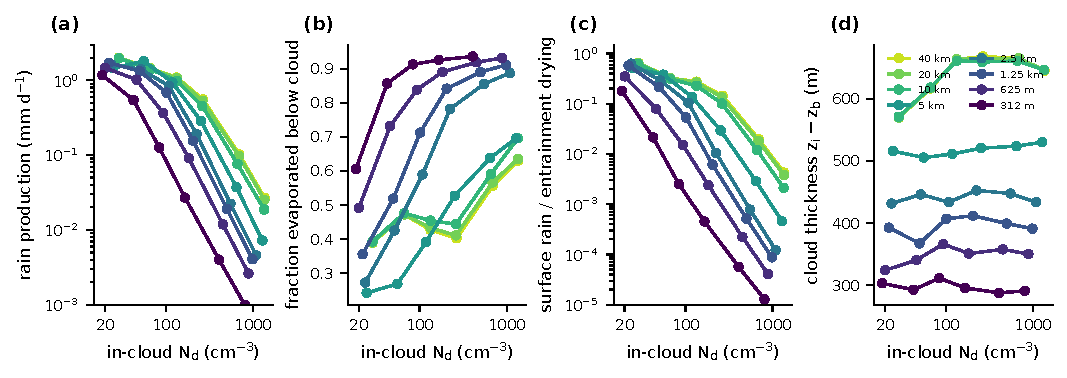
\includegraphics[width=\textwidth]{figures/fig06_rain.pdf}
%DIFDELCMD < \caption{Precipitation budget against in-cloud $\Nd$ at every grid spacing (suppression on, sedimentation factor 1). (a) Column rain production (autoconversion plus accretion). (b) Fraction of the production that evaporates before reaching the surface. (c) Ratio of surface precipitation to the entrainment drying flux. (d) Cloud thickness $\zi-\zb$.}\label{fig:rain}
%DIFDELCMD < \end{figure}
%DIFDELCMD < %%%
\DIFdelend \DIFaddbegin \begin{figure}[t]
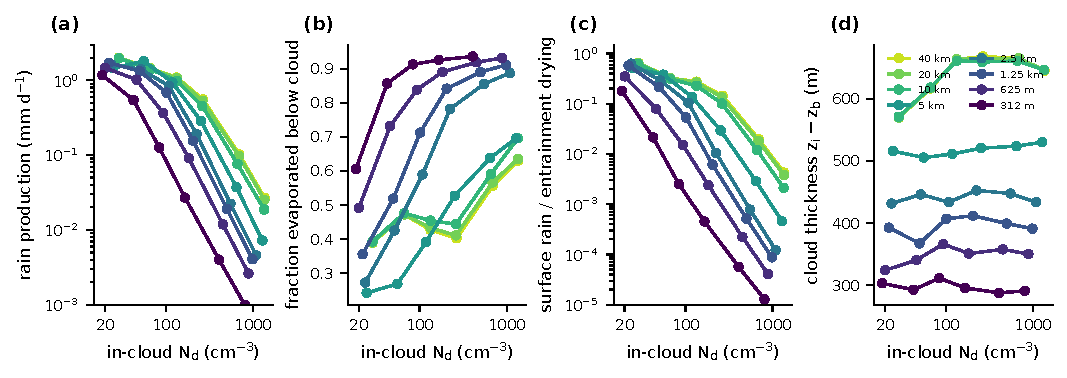
\includegraphics[width=\textwidth]{figures/fig07_rain.pdf}
\caption{Precipitation against in-cloud $\Nd$ at every grid spacing ($\Nd$-dependent autoconversion, sedimentation factor 1). (a) Column rain production. (b) Fraction of the production that evaporates before reaching the surface. (c) Ratio of surface precipitation to entrainment drying. (d) Cloud thickness $\zi-\zb$.}\label{fig:rain}
\end{figure}
\DIFaddend 

\DIFdelbegin %DIFDELCMD < \subsection{Entrainment and the boundary-layer budget}\label{sec:entrain}
%DIFDELCMD < %%%
\DIFdelend \DIFaddbegin \subsection{Drizzle, sedimentation and entrainment}\label{sec:sed}
\DIFaddend 

\DIFdelbegin \DIFdel{At target 200\,$\cmthree$ with suppression on }\DIFdelend \DIFaddbegin \DIFadd{Switching off the $\Nd$ dependence of autoconversion changes LWP through two parts of opposite sign, a rain sink and a drizzle effect on entrainment. In the mixed-layer budget at target $\Nd\geq200\,\cmthree$, removing the heavy drizzle of the $\Nd$-independent runs (that is}\DIFaddend , \DIFdelbegin \DIFdel{the entrainment rate is3.7}\DIFdelend \DIFaddbegin \DIFadd{the difference between the two autoconversion settings) contributes $+4$ to $+6$}\DIFaddend \,\DIFdelbegin \DIFdel{mm}\DIFdelend \DIFaddbegin \DIFadd{\%}\DIFaddend \,\DIFdelbegin \DIFdel{s}\DIFdelend \DIFaddbegin \DIFadd{h}\DIFaddend $^{-1}$ \DIFdelbegin \DIFdel{at 40}\DIFdelend \DIFaddbegin \DIFadd{through the precipitation term at $\dx\geq5$}\DIFaddend \,\DIFdelbegin \DIFdel{km, 7.7\,mm\,s$^{-1}$ at 5\,}\DIFdelend km, \DIFdelbegin \DIFdel{6.8}\DIFdelend \DIFaddbegin \DIFadd{but only $+0.2$ to $+1$}\DIFaddend \,\DIFdelbegin \DIFdel{mm}\DIFdelend \DIFaddbegin \DIFadd{\%}\DIFaddend \,\DIFdelbegin \DIFdel{s}\DIFdelend \DIFaddbegin \DIFadd{h}\DIFaddend $^{-1}$ at \DIFdelbegin \DIFdel{2.5}\DIFdelend \DIFaddbegin \DIFadd{625 and 312}\DIFaddend \,\DIFdelbegin \DIFdel{km, 7.4}\DIFdelend \DIFaddbegin \DIFadd{m. At the same time it raises $\we$ by 0.2}\DIFaddend \,mm\,s$^{-1}$ at \DIFdelbegin \DIFdel{625}\DIFdelend \DIFaddbegin \DIFadd{20--40}\DIFaddend \,\DIFdelbegin \DIFdel{m and 8.1}\DIFdelend \DIFaddbegin \DIFadd{km and by up to 1.4}\DIFaddend \,mm\,s$^{-1}$ at \DIFdelbegin \DIFdel{312}\DIFdelend \DIFaddbegin \DIFadd{$\dx\leq2.5$}\DIFaddend \,\DIFdelbegin \DIFdel{m. The boundary-layer radiative cooling is 80--88\,W\,m$^{-2}$ in all these runs, so the change in $\we$ mostly reflects a change in entrainment efficiency. We define the ratio of entrainment warming to radiative cooling as
}\begin{displaymath}
\DIFdel{\eta = \frac{\rho c_p\we\Delta\theta_l}{F_\mathrm{rad}}.
}\end{displaymath}%DIFAUXCMD
\DIFdel{At $\dx\geq10$\,km , $\eta$ is 0.45--0.67 }\DIFdelend \DIFaddbegin \DIFadd{km }\DIFaddend (Fig.~\ref{fig:entrain}b)\DIFdelbegin \DIFdel{. At $\dx\leq5$\,km it exceeds one for target }\DIFdelend \DIFaddbegin \DIFadd{, consistent with drizzle stabilising the subcloud layer and reducing entrainment \mbox{%DIFAUXCMD
\citep{stevens1998,ackerman2009}}\hskip0pt%DIFAUXCMD
. The difference between the two autoconversion settings therefore measures the precipitation-suppression effect net of a drizzle--entrainment effect, and its small value at fine spacing partly reflects cancellation. The factorial decomposition of Appendix~\ref{app:decomp} shows in addition that the effect of sedimentation on $S$ at coarse spacing depends on the autoconversion formulation, and that the partition between precipitation and sedimentation terms depends on the matching }\DIFaddend $\Nd$ \DIFdelbegin \DIFdel{of 100--200}\DIFdelend \DIFaddbegin \DIFadd{of the $\Nd$-independent configuration.
}

\DIFadd{The offline cloud-top sedimentation flux at $s=1$ is 0.4--1.5}\DIFaddend \,\DIFdelbegin \DIFdel{$\cmthree$ and above, with the largest values at 5}\DIFdelend \DIFaddbegin \DIFadd{mm}\DIFaddend \,\DIFdelbegin \DIFdel{km (1.07}\DIFdelend \DIFaddbegin \DIFadd{d$^{-1}$, with mass-weighted fall speeds of 1.0}\DIFaddend --1\DIFdelbegin \DIFdel{.25 for $\Nd\geq100\,\cmthree$) and at 312}\DIFdelend \DIFaddbegin \DIFadd{.2}\DIFaddend \,\DIFdelbegin \DIFdel{m (1.2--1.3). When $\eta$ exceeds one, entrainment warming exceeds radiative cooling, and with the surface sensible heat flux the mixed layer warms by 0.07--0.10}\DIFdelend \DIFaddbegin \DIFadd{cm}\DIFaddend \,\DIFdelbegin \DIFdel{K\,h}\DIFdelend \DIFaddbegin \DIFadd{s}\DIFaddend $^{-1}$ \DIFdelbegin \DIFdel{at 312}\DIFdelend \DIFaddbegin \DIFadd{at target 1000}\DIFaddend \,\DIFdelbegin \DIFdel{m.
Entrainment drying at 312}\DIFdelend \DIFaddbegin \DIFadd{$\cmthree$, 1.8--2.3}\DIFaddend \,\DIFdelbegin \DIFdel{m (105--131}\DIFdelend \DIFaddbegin \DIFadd{cm}\DIFaddend \,\DIFdelbegin \DIFdel{W}\DIFdelend \DIFaddbegin \DIFadd{s$^{-1}$ at 200}\DIFaddend \,\DIFdelbegin \DIFdel{m$^{-2}$ for $\Nd\geq50\,\cmthree$) likewise exceeds the prescribed latent heat flux of 93}\DIFdelend \DIFaddbegin \DIFadd{$\cmthree$ and 3.8--5.3}\DIFaddend \,\DIFdelbegin \DIFdel{W}\DIFdelend \DIFaddbegin \DIFadd{cm}\DIFaddend \,\DIFdelbegin \DIFdel{m$^{-2}$, whereas at $\dx\geq10$}\DIFdelend \DIFaddbegin \DIFadd{s$^{-1}$ at 20}\DIFaddend \,\DIFdelbegin \DIFdel{km it is 55--78}\DIFdelend \DIFaddbegin \DIFadd{$\cmthree$. Increasing $s$ from 0.5 to 2 raises this flux by 0.5--1.5}\DIFaddend \,\DIFdelbegin \DIFdel{W}\DIFdelend \DIFaddbegin \DIFadd{mm}\DIFaddend \,\DIFdelbegin \DIFdel{m$^{-2}$ (Fig. ~\ref{fig:entrain}c). The response of $\we$ to the sedimentation factor at fixed $\Nd$ }\DIFdelend \DIFaddbegin \DIFadd{d$^{-1}$ at target $\Nd\geq200\,\cmthree$ at all grid spacings }\DIFaddend (Fig.~\ref{fig:entrain}a)\DIFdelbegin \DIFdel{is largest at $\dx\leq5$}\DIFdelend \DIFaddbegin \DIFadd{. At $\dx\leq2.5$}\DIFaddend \,km \DIFdelbegin \DIFdel{and low $\Nd$, where doubling the fall speed relative to $s=0.5$ reduces }\DIFdelend \DIFaddbegin \DIFadd{this increase is accompanied by a decrease of }\DIFaddend $\we$ by \DIFdelbegin \DIFdel{1.1--2.4}\DIFdelend \DIFaddbegin \DIFadd{0.2--1.2}\DIFaddend \,mm\,s$^{-1}$ \DIFdelbegin \DIFdel{at target $\Nd\leq50\,\cmthree$; at target $\Nd\geq500\,\cmthree$ the reduction is 0.2--0.8}\DIFdelend \DIFaddbegin \DIFadd{(regression slope $-0.8$}\DIFaddend \,mm\,s$^{-1}$ \DIFdelbegin \DIFdel{. At }\DIFdelend \DIFaddbegin \DIFadd{per mm\,d$^{-1}$, correlation $-0.31$), whereas at }\DIFaddend $\dx\geq10$\,km \DIFdelbegin \DIFdel{the reduction is less than 0.6}\DIFdelend \DIFaddbegin \DIFadd{$\we$ does not respond (slope $-0.03$). The sedimentation--entrainment coupling of \mbox{%DIFAUXCMD
\citet{bretherton2007} }\hskip0pt%DIFAUXCMD
thus operates at $\dx\leq2.5$}\DIFaddend \,\DIFaddbegin \DIFadd{km and is absent at coarse spacing, where the inversion is pinned. At low $\Nd$ the larger decrease of $\we$ with $s$ (1.1--2.4\,}\DIFaddend mm\,s$^{-1}$ at \DIFdelbegin \DIFdel{all $\Nd$. This is the expected sign }\DIFdelend \DIFaddbegin \DIFadd{$\dx\leq5$\,km) occurs together with large fall speeds and drizzle, so it is not a clean measure }\DIFaddend of the sedimentation--entrainment \DIFdelbegin \DIFdel{feedback \mbox{%DIFAUXCMD
\citep{bretherton2007,ackerman2009}}\hskip0pt%DIFAUXCMD
, and its larger magnitude }\DIFdelend \DIFaddbegin \DIFadd{coupling. Because P3 sedimentation acts after SHOC's adjustment within each step and the cloud-top fields are written after P3, the time step (100\,s at coarse and 15\,s }\DIFaddend at fine spacing\DIFdelbegin \DIFdel{indicates that the coupling between sedimentation and entrainment is stronger where part of the boundary-layer circulation is resolved}\DIFdelend \DIFaddbegin \DIFadd{) may also affect how much cloud-top liquid is removed per step; cloud-top $\Nd$ relative to the target decreases with $s$ by 8--12\,\% at 40\,km but not at 312\,m}\DIFaddend .

\DIFdelbegin %DIFDELCMD < \begin{figure}[t]
%DIFDELCMD < 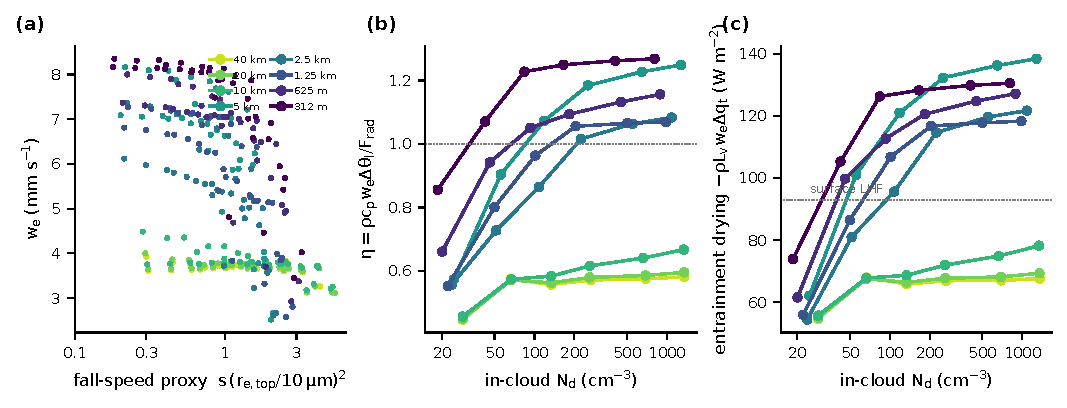
\includegraphics[width=\textwidth]{figures/fig07_entrainment.pdf}
%DIFDELCMD < \caption{(a) Change in the entrainment rate between sedimentation factors 2 and 0.5 at fixed target $\Nd$ (suppression on). (b) Ratio $\eta$ of entrainment warming to boundary-layer radiative cooling and (c) entrainment drying flux, with the prescribed surface latent heat flux (dotted line), for suppression on and sedimentation factor 1.}\label{fig:entrain}
%DIFDELCMD < \end{figure}
%DIFDELCMD < %%%
\DIFdelend \DIFaddbegin \begin{figure}[t]
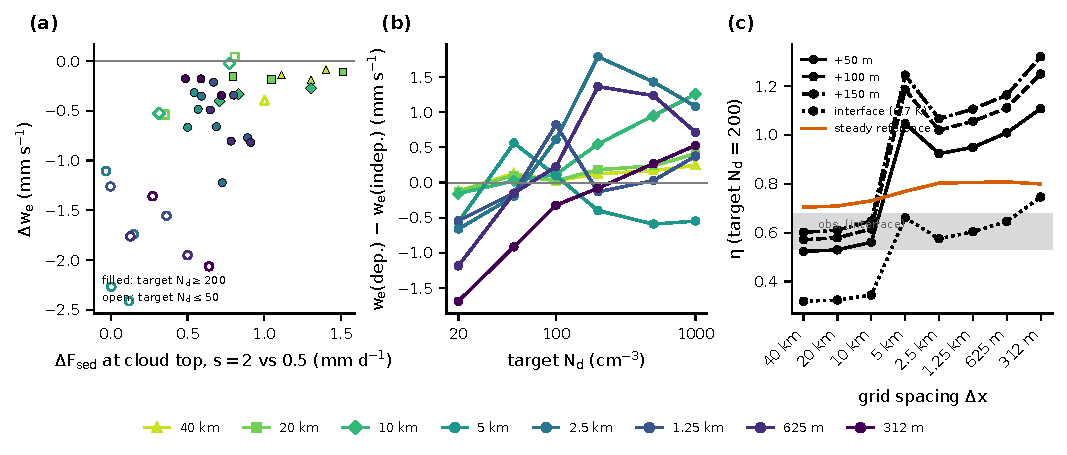
\includegraphics[width=\textwidth]{figures/fig08_entrainment.pdf}
\caption{(a) Change in entrainment rate against change in the offline cloud-top sedimentation flux between sedimentation factors 2 and 0.5 ($\Nd$-dependent autoconversion); filled symbols target $\Nd\geq200\,\cmthree$, open symbols $\leq50\,\cmthree$. (b) Difference in entrainment rate between $\Nd$-dependent and $\Nd$-independent autoconversion (sedimentation factor 1). (c) $\eta$ at target $\Nd=200\,\cmthree$ for jumps taken 50, 100 and 150\,m above $\zi$ and for the specified interface jump, with the steady-state reference and the observed range for the interface definition.}\label{fig:entrain}
\end{figure}
\DIFaddend 

\DIFdelbegin \DIFdel{The mixed-layer budget (Sect.~\ref{sec:mlb}) expresses these fluxes as contributions to the LWP tendency }\DIFdelend \DIFaddbegin \subsection{Decoupling and the mixed-layer budget}\label{sec:budget}

\DIFadd{The degree of coupling depends on the metric }\DIFaddend (Fig.~\DIFdelbegin \DIFdel{\ref{fig:budget}). In every run, radiative cooling and surface fluxes thicken the cloud, and entrainment and subsidence thin it. At 40}\DIFdelend \DIFaddbegin \DIFadd{\ref{fig:decoup}). The coarse runs have the largest moisture difference across the boundary layer ($\Delta q_t=1.1$--1.5}\DIFaddend \,\DIFdelbegin \DIFdel{km, where the budget reproduces both the tendencies and their differences between $\Nd$ levels (Table~\ref{tab:skill}), }\DIFdelend \DIFaddbegin \DIFadd{g\,kg$^{-1}$), produced by SHOC's down-gradient transport of the surface moisture flux, but their $\theta_l$ is well mixed, }\DIFaddend the \DIFdelbegin \DIFdel{entrainment contribution is about $-9$}\DIFdelend \DIFaddbegin \DIFadd{buoyancy flux below cloud base stays at 40--110}\DIFaddend \,\DIFdelbegin \DIFdel{\%}\DIFdelend \DIFaddbegin \DIFadd{\% of its surface value and cloud base lies within 35}\DIFaddend \,\DIFdelbegin \DIFdel{h$^{-1}$ at all $\Nd$, and the precipitation contribution decreases in magnitude from $-10$\,\%\,h$^{-1}$ at target 20\,$\cmthree$ to nearly zero at $\Nd\geq500\,\cmthree$. The increase of LWP with $\Nd$ at 40\,km is therefore associated with the removal of the precipitation sink, consistent with Sect. ~\ref{sec:attr}. }\DIFdelend \DIFaddbegin \DIFadd{m of the mixed-layer condensation level, so they are coupled by the Jones test and by the flux criterion. }\DIFaddend At 312\,m \DIFdelbegin \DIFdel{, the entrainment contribution is about three times larger ($-27$ to $-32$}\DIFdelend \DIFaddbegin \DIFadd{and target $\Nd\geq100\,\cmthree$, $\Delta q_t$ is only 0.2--0.3}\DIFaddend \,\DIFdelbegin \DIFdel{\%}\DIFdelend \DIFaddbegin \DIFadd{g}\DIFaddend \,\DIFdelbegin \DIFdel{h}\DIFdelend \DIFaddbegin \DIFadd{kg}\DIFaddend $^{-1}$\DIFdelbegin \DIFdel{for $\Nd\geq50\,\cmthree$), and it is partly offset by larger radiative (21--24}\DIFdelend \DIFaddbegin \DIFadd{, but the buoyancy-flux minimum below cloud base is 8--10}\DIFaddend \,\% \DIFaddbegin \DIFadd{of the surface value, cloud base lies 50--70}\DIFaddend \,\DIFdelbegin \DIFdel{h$^{-1}$) and surface-flux (12--13}\DIFdelend \DIFaddbegin \DIFadd{m above the mixed-layer condensation level, and the variance is concentrated below cloud. Refinement therefore increases decoupling by the buoyancy-flux and cloud-base metrics while decreasing it by $\Delta q_t$. The buoyancy flux is not significantly negative below cloud base in any run, so the low-$\Nd$ states resemble cumulus rising into stratocumulus, without a stable subcloud layer.
}

\begin{figure}[t]
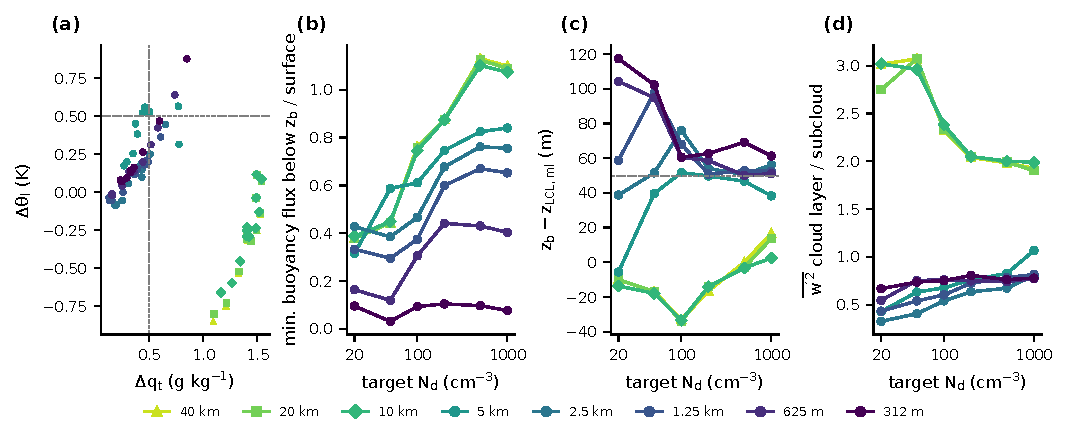
\includegraphics[width=\textwidth]{figures/fig10_decoupling.pdf}
\caption{Decoupling metrics (sedimentation factor 1, hours 10--12). (a) $\Delta\theta_l$ against $\Delta q_t$ between the highest and lowest quarters of the layer below the inversion base for both autoconversion settings, with the thresholds of \citet{jones2011}. (b) Minimum total buoyancy flux below cloud base relative to the surface value, (c) cloud base above the mixed-layer lifting condensation level, and (d) ratio of cloud-layer to subcloud vertical-velocity variance, for $\Nd$-dependent autoconversion.}\label{fig:decoup}
\end{figure}

\DIFadd{By the combined criterion of Sect.~\ref{sec:mlb}, 97}\DIFaddend \,\% \DIFaddbegin \DIFadd{of the 2}\DIFaddend \,h \DIFdelbegin \DIFdel{$^{-1}$) contributions; the precipitation contribution is below 1}\DIFdelend \DIFaddbegin \DIFadd{windows at $\dx\geq10$}\DIFaddend \,\DIFdelbegin \DIFdel{\%}\DIFdelend \DIFaddbegin \DIFadd{km are coupled, 58}\DIFaddend \,\DIFdelbegin \DIFdel{h$^{-1}$ in magnitude for $\Nd\geq100\,\cmthree$. The budget sum is negative at all $\Nd$ ($-2$ to $-5$\,}\DIFdelend \% \DIFaddbegin \DIFadd{at 5}\DIFaddend \,\DIFdelbegin \DIFdel{h$^{-1}$), consistent in sign and magnitude with the simulated thinning ($-4$ to $-6$}\DIFdelend \DIFaddbegin \DIFadd{km, 11}\DIFaddend \,\DIFdelbegin \DIFdel{\%}\DIFdelend \DIFaddbegin \DIFadd{\% at 2.5}\DIFaddend \,\DIFdelbegin \DIFdel{h$^{-1}$). At 625}\DIFdelend \DIFaddbegin \DIFadd{km and at most 3}\DIFaddend \,\DIFdelbegin \DIFdel{m the budget sum at high $\Nd$ ($-5.4$ to $-5.7$\,}\DIFdelend \% \DIFaddbegin \DIFadd{at $\dx\leq1.25$}\DIFaddend \,\DIFdelbegin \DIFdel{h$^{-1}$) is more negative than the simulated trend ($-1.9$ to $-2.9$\,\% \,h$^{-1}$). The budget therefore suggests that the general thinning at fine grid spacingis associated with }\DIFdelend \DIFaddbegin \DIFadd{km. The mixed-layer budget (Fig.~\ref{fig:budget}) is therefore used for attribution only at coarse spacing. There it reproduces the in-cloud LWP tendency in coupled windows with correlations of 0.72--0.76, and }\DIFaddend the increase of \DIFdelbegin \DIFdel{entrainment relative to the radiative and surface forcing. At $\dx\leq2.5$}\DIFdelend \DIFaddbegin \DIFadd{LWP with $\Nd$ at 40}\DIFaddend \,km \DIFdelbegin \DIFdel{, however, the net $\Nd$ dependence of the budget sum (about 2}\DIFdelend \DIFaddbegin \DIFadd{follows from the removal of the precipitation sink ($-10$}\DIFaddend \,\%\,h$^{-1}$ at \DIFdelbegin \DIFdel{312}\DIFdelend \DIFaddbegin \DIFadd{target 20}\DIFaddend \,\DIFdelbegin \DIFdel{m) is no larger than the budget error}\DIFdelend \DIFaddbegin \DIFadd{$\cmthree$ and nearly zero at $\geq500\,\cmthree$) at an entrainment contribution that is constant in $\Nd$. At 2.5\,km and finer the correlation for in-cloud LWP falls to 0.47 and 0.07--0.32}\DIFaddend , and the entrainment \DIFdelbegin \DIFdel{term itself varies non-monotonically with $\Nd$ ($-29$, $-29$, $-27$, $-31$ and $-32$}\DIFdelend \DIFaddbegin \DIFadd{contribution splits into a deepening part of $+10$ to $+20$}\DIFaddend \,\%\,h$^{-1}$ \DIFdelbegin \DIFdel{for targets 50 to 1000}\DIFdelend \DIFaddbegin \DIFadd{and a cloud-base part of $-30$ to $-50$}\DIFaddend \,\DIFdelbegin \DIFdel{$\cmthree$ }\DIFdelend \DIFaddbegin \DIFadd{\%\,h$^{-1}$ }\DIFaddend at 312\,m\DIFdelbegin \DIFdel{)}\DIFdelend \DIFaddbegin \DIFadd{, so the net thinning is the small difference of large terms in a decoupled layer}\DIFaddend . The budget \DIFaddbegin \DIFadd{is consistent with the view that stronger entrainment raises cloud base faster than it deepens the layer at fine spacing, but it }\DIFaddend does not establish which process sets the small negative susceptibilities \DIFdelbegin \DIFdel{at sub-kilometre spacing}\DIFdelend \DIFaddbegin \DIFadd{there}\DIFaddend .

\DIFdelbegin %DIFDELCMD < \begin{figure}[t]
%DIFDELCMD < 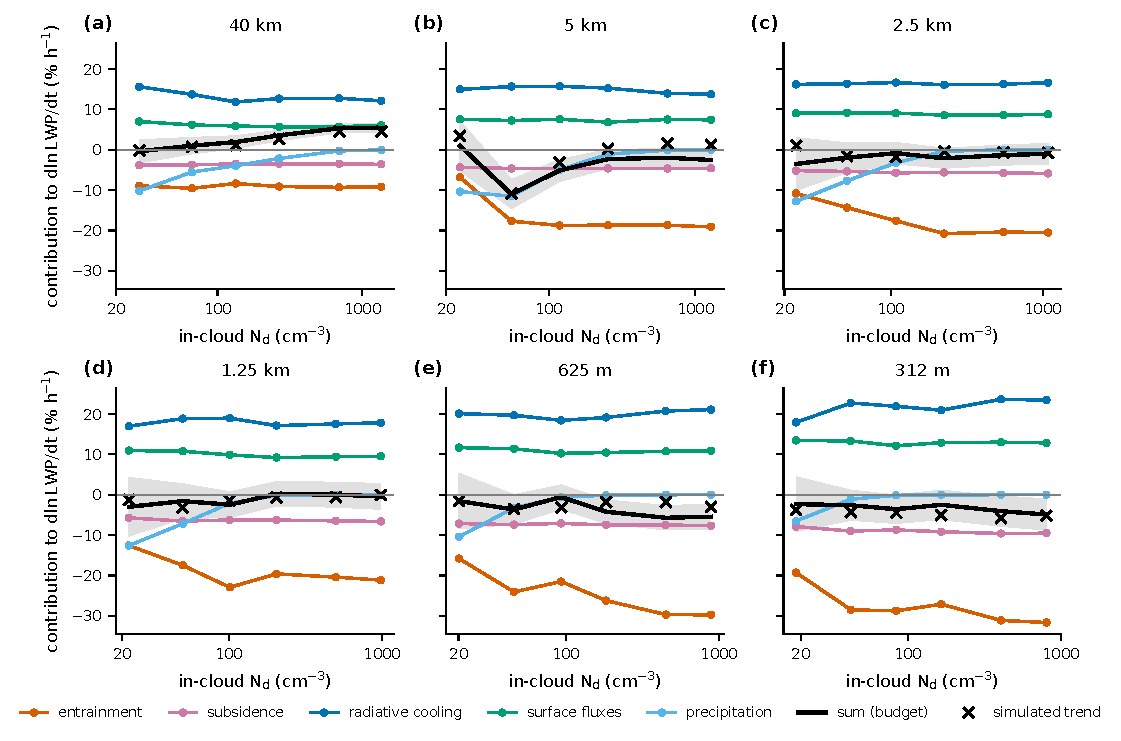
\includegraphics[width=\textwidth]{figures/fig08_budget.pdf}
%DIFDELCMD < \caption{Mixed-layer LWP budget (Eq.~\ref{eq:lwpbudget}) for hours 10--12, expressed as contributions to $d\ln\LWP/dt$, at (a) 40\,km, (b) 5\,km, (c) 2.5\,km, (d) 1.25\,km, (e) 625\,m and (f) 312\,m (suppression on, sedimentation factor 1). The black line is the budget sum, with shading of $\pm$ the root-mean-square error of the budget at that grid spacing (Table~\ref{tab:skill}); crosses are the simulated LWP trend. The entrainment rate in the budget is diagnosed over each 2\,h window, whereas Figs.~\ref{fig:response} and \ref{fig:entrain} use the 8--12\,h fit.}\label{fig:budget}
%DIFDELCMD < \end{figure}
%DIFDELCMD < %%%
\DIFdelend \DIFaddbegin \begin{figure}[t]
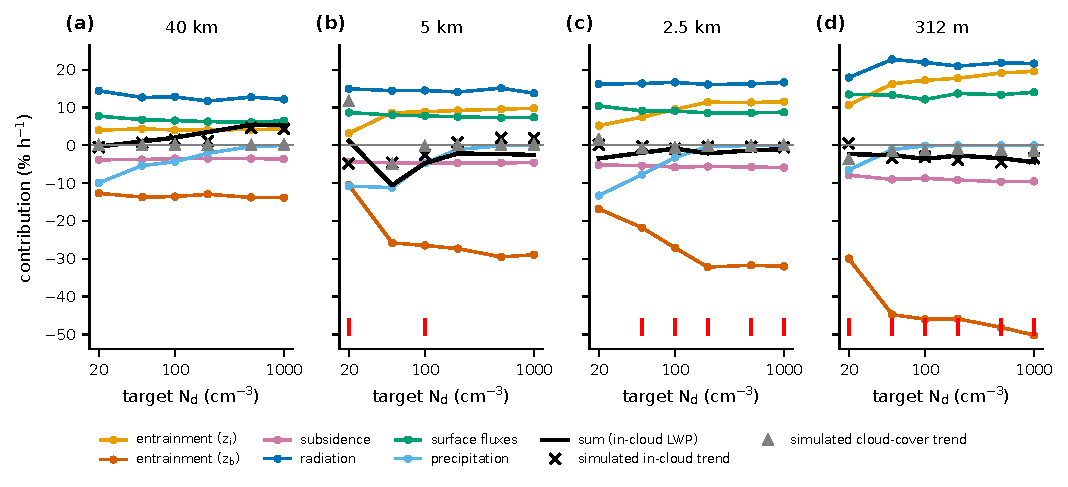
\includegraphics[width=\textwidth]{figures/fig09_budget.pdf}
\caption{Mixed-layer budget of in-cloud LWP for hours 10--12 at (a) 40\,km, (b) 5\,km, (c) 2.5\,km and (d) 312\,m ($\Nd$-dependent autoconversion, sedimentation factor 1), with the entrainment term split into deepening and cloud-base parts. Crosses and triangles are the simulated tendencies of in-cloud LWP and cloud cover. Red ticks mark windows that fail the coupling criterion, for which the attribution is not valid.}\label{fig:budget}
\end{figure}
\DIFaddend 

\DIFdelbegin %DIFDELCMD < \subsection{Subgrid and resolved turbulence}\label{sec:grey}
%DIFDELCMD < %%%
\DIFdelend \DIFaddbegin \subsection{Robustness}\label{sec:robust}
\DIFaddend 

\DIFdelbegin \DIFdel{At $\dx\geq10$\,km, all vertical-velocity variance is parameterised (Fig.~\ref{fig:structure}a), and SHOC's boundary-layer variance lies between 0.28 and 0.41\,m$^2$\,s$^{-2}$. At 5 and 2.5\,km this variance is 0.07}\DIFdelend \DIFaddbegin \DIFadd{The perturbed twins give standard deviations of the differences in $S$ of 0.007}\DIFaddend --0\DIFdelbegin \DIFdel{.11\,m$^2$\,s$^{-2}$, and it decreases to 0.03\,m$^2$\,s$^{-2}$ at 312\,m, while the resolved variance increases. The resolved share of the total is 3--7\,\% at 5\,km, 4--9\,\% at 2.5\,km, 9--19\,\% at 1.25\,km, 28--38\,\% at }\DIFdelend \DIFaddbegin \DIFadd{.010 on the clean, middle and moderate branches and 0.002--0.004 on the polluted branch at }\DIFaddend 625 \DIFdelbegin \DIFdel{\,m and 54--67\,\% at 312\,m, so that a third of the variance remains subgrid even at 312\,m. Part of this repartition is imposed by the closure. SHOC's mixing length is capped at the nominal grid spacing, }\DIFdelend and \DIFdelbegin \DIFdel{at }\DIFdelend 312\,\DIFdelbegin \DIFdel{m the domain-mean mixing length is within 5\,\% of this cap at 90\,\% of the boundary-layer levels, compared with 25\,\% at 625\,m and none at $\dx\geq1.25$\,km (Appendix~\ref{app:shoc}, Fig.~\ref{fig:shocmix}a). At 312\,}\DIFdelend m, \DIFdelbegin \DIFdel{SHOC's eddy diffusivity is therefore directly limited by the grid spacing throughout the boundary layer. The large change between 10 }\DIFdelend \DIFaddbegin \DIFadd{so a single run has a noise of about 0.007 }\DIFaddend and \DIFaddbegin \DIFadd{0.002, respectively. The tile bootstrap gives similar values at sub-kilometre spacing (0.006 and 0.003) and up to 0.03 at }\DIFaddend 5\,\DIFdelbegin \DIFdel{km, where the resolved share is still small, is also not explained by resolved turbulence. At 5\,km SHOC's boundary-layer mean mixing length is about two thirds of its value at 10\,km (Fig.~\ref{fig:shocmix}a ), even though the cap is not active, which points to a change in the SHOC solution itself, possibly coupled to the stripe-like circulations noted in Sect. ~\ref{sec:morph}. We have not diagnosed this transition further.
}%DIFDELCMD < 

%DIFDELCMD < %%%
\DIFdel{The resolved vertical-velocity skewness (Fig.~\ref{fig:structure}b), which is meaningful only at $\dx\leq5$\,km, is positive at low $\Nd$ (up to 1.9 at }\DIFdelend \DIFaddbegin \DIFadd{km. The moderate-branch value at }\DIFaddend 312\,\DIFdelbegin \DIFdel{m for target 20\,$\cmthree$) , indicating narrow, strong updrafts in a drizzle-decoupled boundary layer. At high $\Nd$ it is $-0.7$ to $-1.0$ at 2.5 and 1.25\,km and $-0.3$ to $-0.7$ at 625\,m, the sign expected for radiatively driven downdrafts in a well-mixed stratocumulus layer \mbox{%DIFAUXCMD
\citep{wood2012}}\hskip0pt%DIFAUXCMD
; the transition occurs at $\Nd\approx50$--$100\,\cmthree$. At 312\,}\DIFdelend m \DIFdelbegin \DIFdel{the skewness stays positive at all $\Nd$ (0.09--0.24 for target $\Nd\geq100\,\cmthree$) . With a third of the variance still subgrid and the mixing length at its cap, this may reflect near-grid-scale updrafts. Drizzle decouples the boundary layer at low $\Nd$ (Fig.~\ref{fig:structure}c). At $\dx\leq5$\,km, $\Delta q_t$ is 1.1--1.6\,g\,kg$^{-1}$ at target 20\,$\cmthree$ }\DIFdelend \DIFaddbegin \DIFadd{($-0.05$, negative for all three sedimentation factors and both autoconversion settings) }\DIFaddend and \DIFdelbegin \DIFdel{0.21--0.64}\DIFdelend \DIFaddbegin \DIFadd{the polluted-branch values at $\dx\leq2.5$}\DIFaddend \,\DIFdelbegin \DIFdel{g\,kg$^{-1}$ at 1000\,$\cmthree$, consistent with below-cloud evaporation stabilising the subcloud layer \mbox{%DIFAUXCMD
\citep{stevens1998,bretherton1997,jones2011}}\hskip0pt%DIFAUXCMD
. In the single-column limit, $q_t$ decreases upward by 1.2--1.7\,g\,kg$^{-1}$ at all $\Nd$ across a deep cloud layer.
}%DIFDELCMD < 

%DIFDELCMD < %%%
\DIFdel{The LWP spectral peak changes less between }\DIFdelend \DIFaddbegin \DIFadd{km are therefore well outside the internal noise. The moderate branch at }\DIFaddend 625\DIFdelbegin \DIFdel{and 312}\DIFdelend \,m \DIFdelbegin \DIFdel{than LWP itself (Fig.~\ref{fig:structure}d; Appendix~\ref{app:spectra}) . At 5 and 2.5\,km the peak wavelengths of 48 and 30\,km correspond to 6.4 and 8 physics-column spacings and are probably limited by the effective resolution of the dynamical core. At 625 and 312\,m the peak lies at 13--22\,km, an aspect ratio $\lambda/\zi$ of 13--20. Observed closed mesoscale cells have aspect ratios of up to about 30--40 for boundary layers about 1\,km deep \mbox{%DIFAUXCMD
\citep{wood2006}}\hskip0pt%DIFAUXCMD
, and LES with large domains also produce cells that are wider than these \mbox{%DIFAUXCMD
\citep{kazil2017,zhou2018,zhou2019b}}\hskip0pt%DIFAUXCMD
.The sub-kilometre cells are therefore on the narrow side of the observed range, and }\DIFdelend \DIFaddbegin \DIFadd{(0.03) changes sign with the autoconversion setting, and }\DIFaddend the \DIFdelbegin \DIFdel{2.5\,km value (33) agrees better with the observations, although it is probably resolution-limited. }%DIFDELCMD < 

%DIFDELCMD < %%%
\DIFdel{Switching on 3D turbulence }\DIFdelend \DIFaddbegin \DIFadd{location of the LWP maximum is not resolvable. The main threats to the fine-grid results are thus transience (Sect.~\ref{sec:time}) and structural choices, in particular the fixed vertical grid and the mixing-length cap, rather than internal variability. The 3D-turbulence option }\DIFaddend changes LWP by less than 1.5\,\DIFdelbegin \DIFdel{$\gmm$ ($<1.5$\,\% ), cloud cover by less than 0.007 }\DIFdelend \DIFaddbegin \DIFadd{\% }\DIFaddend and $\we$ by \DIFdelbegin \DIFdel{$-0.13$ to $+0.02$}\DIFdelend \DIFaddbegin \DIFadd{less than 0.13}\DIFaddend \,mm\,s$^{-1}$ \DIFdelbegin \DIFdel{at 625\,m and 312\,m }\DIFdelend (Appendix~\ref{app:t3d}).
\DIFdelbegin \DIFdel{The 3D turbulence option therefore has a negligible effect on the results, which is expected because SHOC's horizontal diffusion is small compared with the horizontal dissipation of the dynamical core.
}\DIFdelend 

\DIFdelbegin %DIFDELCMD < \begin{figure}[t]
%DIFDELCMD < 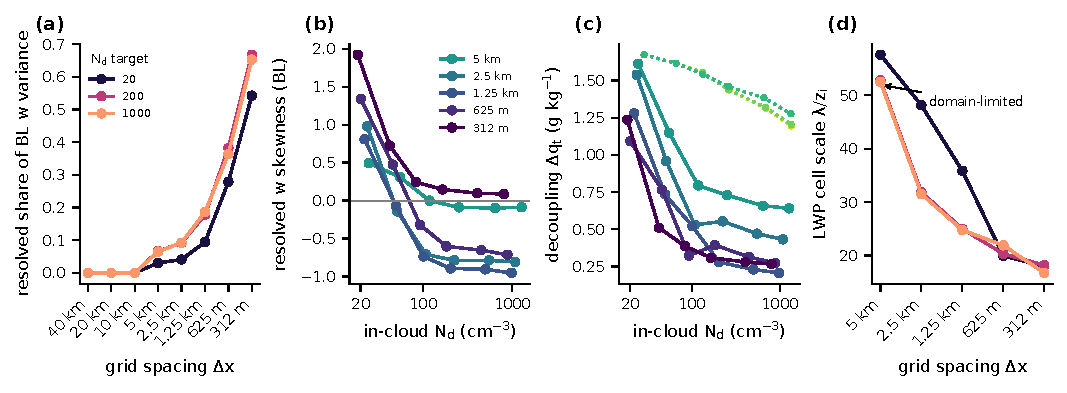
\includegraphics[width=\textwidth]{figures/fig09_structure.pdf}
%DIFDELCMD < \caption{Boundary-layer structure (suppression on, sedimentation factor 1). (a) Resolved share of boundary-layer vertical-velocity variance against grid spacing for three target $\Nd$. (b) Resolved vertical-velocity skewness over the boundary layer ($\dx\leq5$\,km). (c) Decoupling $\Delta q_t$ against in-cloud $\Nd$ (dotted lines: $\dx\geq10$\,km). (d) LWP spectral peak wavelength relative to $\zi$ ($\dx\leq5$\,km).}\label{fig:structure}
%DIFDELCMD < \end{figure}
%DIFDELCMD < %%%
\DIFdelend %DIF > % ====================================================================
\DIFaddbegin \section{Discussion}\label{sec:discussion}
%DIF > % ====================================================================
\DIFaddend 

\DIFdelbegin %DIFDELCMD < \subsection{Convergence}\label{sec:conv}
%DIFDELCMD < %%%
\DIFdelend \DIFaddbegin \subsection{One mixed-layer argument}
\DIFaddend 

\DIFdelbegin \DIFdel{None of the bulk quantities converges with grid spacing (Fig.~\ref{fig:conv}). At fixed diagnosed $\Nd$, LWP decreases by 10--23\,\% from 1.25\,km to 625\,m and by a further 21--40\,\% from 625 to 312\,m, the larger decreases occurring at higher $\Nd$. The maximum-overlap cloud cover and }\DIFdelend \DIFaddbegin \DIFadd{The results can be summarised by a single chain. Grid spacing changes the entrainment rate (Sect.~\ref{sec:regimes}); the entrainment rate sets the depth and base height of the cloud and hence its rain production and the fraction of rain that evaporates (Sect.~\ref{sec:regime}); and the resulting ratio of precipitation to entrainment drying sets the moderate-branch susceptibility, as in }\DIFaddend the \DIFdelbegin \DIFdel{cloud thickness also continue to decrease. For LWP at target $\Nd\geq50\,\cmthree$, the change over the last halving of the grid spacing exceeds that over the previous one by a factor of 1.3--2.0, so the sequence is not in an asymptotic range and an extrapolation to zero grid spacing is not meaningful. The entrainment rate is non-monotonic, with a minimum at 2.5--1.25\,km, as expected in the grey zone where parameterised and resolved contributions trade places \mbox{%DIFAUXCMD
\citep{honnert2020,boutle2014}}\hskip0pt%DIFAUXCMD
. The clean-branch susceptibility (0.65--0.76 }\DIFdelend \DIFaddbegin \DIFadd{mixed-layer arguments of \mbox{%DIFAUXCMD
\citet{ackerman2004}}\hskip0pt%DIFAUXCMD
, \mbox{%DIFAUXCMD
\citet{wood2007} }\hskip0pt%DIFAUXCMD
and \mbox{%DIFAUXCMD
\citet{hoffmann2020}}\hskip0pt%DIFAUXCMD
. At coarse spacing the sink removed by precipitation suppression is large and the response is positive; }\DIFaddend at \DIFdelbegin \DIFdel{$\dx\leq2.5$}\DIFdelend \DIFaddbegin \DIFadd{fine spacing there is little rain to suppress, the sedimentation--entrainment coupling becomes active and the response is near zero or slightly negative. Most of the resolution dependence of $\Shigh$ is thus a dependence on the simulated cloud regime, which grid spacing controls in EAMxx; at fixed regime, grid spacing adds little explanatory power on this branch. The near-zero susceptibility at fine spacing reflects an absent precipitation sink, which differs from the compensation between processes that \mbox{%DIFAUXCMD
\citet{stevens2009} }\hskip0pt%DIFAUXCMD
described as buffering. Two parts of the response do not follow this chain, namely the cloud-cover response on the clean branch, which is absent at coarse spacing by construction and which dominates the radiative relevance at fine spacing, and the polluted branch, which retains a dependence on grid spacing at nearly zero precipitation.
}

\DIFadd{The first link of the chain is the least physical. Entrainment changes abruptly between 10 and 5}\DIFaddend \,\DIFdelbegin \DIFdel{km) varies less with grid spacing than the bulk quantities, but it varies with $s$ from 0.56 to 0.97 at 312\,m. The vertical grid (about 50\,m at the inversion, compared with about }\DIFdelend \DIFaddbegin \DIFadd{km as the }\DIFaddend 5\,\DIFdelbegin \DIFdel{m in the RF02 LES; \mbox{%DIFAUXCMD
\citealp{ackerman2009}}\hskip0pt%DIFAUXCMD
) was held fixed, and vertical resolution at the inversion is known to control entrainment in LES and in SCREAM \mbox{%DIFAUXCMD
\citep{stevens2005,bogenschutz2023rrm}}\hskip0pt%DIFAUXCMD
. The sign of $\Shigh$ }\DIFdelend \DIFaddbegin \DIFadd{km runs leave a state pinned at the inversion, and }\DIFaddend at \DIFdelbegin \DIFdel{312}\DIFdelend \DIFaddbegin \DIFadd{5}\DIFaddend \,\DIFdelbegin \DIFdel{m may change with further horizontal or vertical refinement. }%DIFDELCMD < 

%DIFDELCMD < \begin{figure}[t]
%DIFDELCMD < 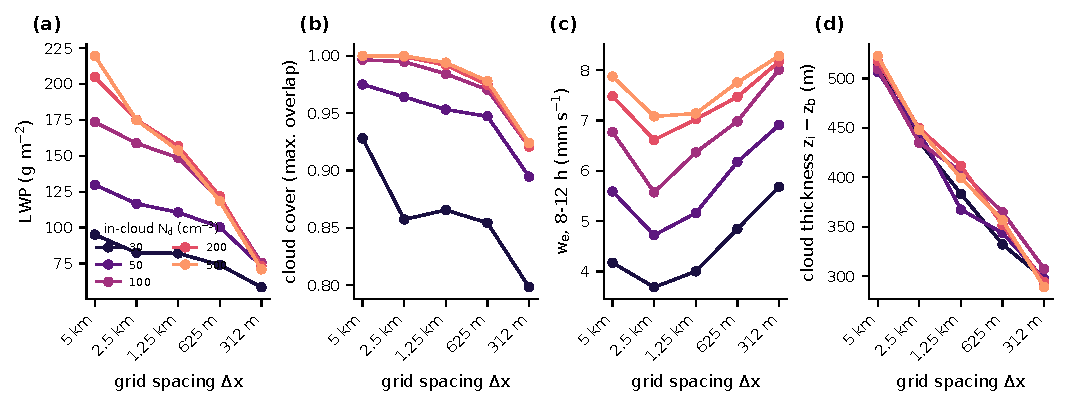
\includegraphics[width=\textwidth]{figures/fig10_convergence.pdf}
%DIFDELCMD < \caption{Hour 10--12 means against grid spacing ($\dx\leq5$\,km) at fixed diagnosed in-cloud $\Nd$, interpolated in $\ln\Nd$ (suppression on, sedimentation factor 1). (a) LWP, (b) maximum-overlap cloud cover including SHOC's subgrid cloud fraction, (c) entrainment rate (8--12\,h fit) and (d) cloud thickness.}\label{fig:conv}
%DIFDELCMD < \end{figure}
%DIFDELCMD < 

%DIFDELCMD < \subsection{Cloud-top droplet number and within-scene covariability}\label{sec:sat}
%DIFDELCMD < 

%DIFDELCMD < %%%
\DIFdel{Satellite estimates of LWP adjustments use $\Nd$ retrieved from cloud-top effective radius and optical depth under adiabatic assumptions \mbox{%DIFAUXCMD
\citep{grosvenor2018}}\hskip0pt%DIFAUXCMD
. The model-diagnosed cloud-top $\Nd$ used here is not such a retrieval. It is 44--72}\DIFdelend \DIFaddbegin \DIFadd{km the resolved flow is dominated by near-grid-scale motions. At $\dx\leq2.5$}\DIFaddend \,\DIFdelbegin \DIFdel{\% of the in-cloud layer value at $\dx\geq10$\,km and 77--95\,\% at 312\,m, and because this ratio varies little with $\Nd$ at a given grid spacing , susceptibilities computed with cloud-top $\Nd$ differ from those computed with layer $\Nd$ by at most 0.10, 0.04 and 0.01 on the three branches (Fig. ~\ref{fig:sat}a). This agreement follows largely from the near-constant ratio and says nothing about retrieval errors. }%DIFDELCMD < 

%DIFDELCMD < %%%
\DIFdel{Within each domain CCN are horizontally uniform, so the spatial covariation of LWP and cloud-top $\Nd$ arises from cloud processes. We regressed column $\ln\LWP$ on column cloud-top $\ln\Nd$ over cloudy columns at each 15\,min instant in hours 10--12, restricting the analysis to $\dx\leq5$\,km because the columns at coarser spacingare nearly identical.
The slopes range from $-7.9$ to $+3.4$, with standard errors over instants of at most 0.8 and correlations between $-0.86$ and $+0.56$ (Fig.~\ref{fig:sat}c). At 2.5--5\,}\DIFdelend km \DIFdelbegin \DIFdel{and low $\Nd$ they are negative, because collision--coalescence depletes $\Nd$ in the thickest, drizzling columns (Fig.~\ref{fig:sat}b). At 625 and 312\,m and target $\Nd\geq50\,\cmthree$ they are positive (0.4--3.3), because }\DIFdelend \DIFaddbegin \DIFadd{about half of the inferred entrainment flux is not carried by resolved or parameterised turbulence, the inversion spans two to three levels and }\DIFaddend cloud-top \DIFdelbegin \DIFdel{$\Nd$ is reduced in thin, evaporating cloud edges. At 312}\DIFdelend \DIFaddbegin \DIFadd{height varies by less than one level. LES studies show that entrainment converges from above as the inversion is resolved \mbox{%DIFAUXCMD
\citep{stevens1999res,stevens2005,pressel2017,mellado2018}}\hskip0pt%DIFAUXCMD
. Our sub-kilometre runs, with fixed 50}\DIFaddend \,\DIFdelbegin \DIFdel{m and target 200\,$\cmthree$, for example, the within-scene slope is $+1.9$, whereas $\Shigh=-0.05$. That cloud-controlled $\Nd$ variability produces spatial LWP--$\Nd$ relationships unrelated to the causal response is well established \mbox{%DIFAUXCMD
\citep{gryspeerdt2019,arola2022,mulmenstadt2024gcm,mahfouz2024}}\hskip0pt%DIFAUXCMD
. The additional result here is that the sign of this covariation changes with grid spacing, because the relative importance of drizzle depletion in thick cloud and evaporation in thin cloud edges depends on how much of the cloud field is resolved.
}%DIFDELCMD < 

%DIFDELCMD < \begin{figure}[t]
%DIFDELCMD < 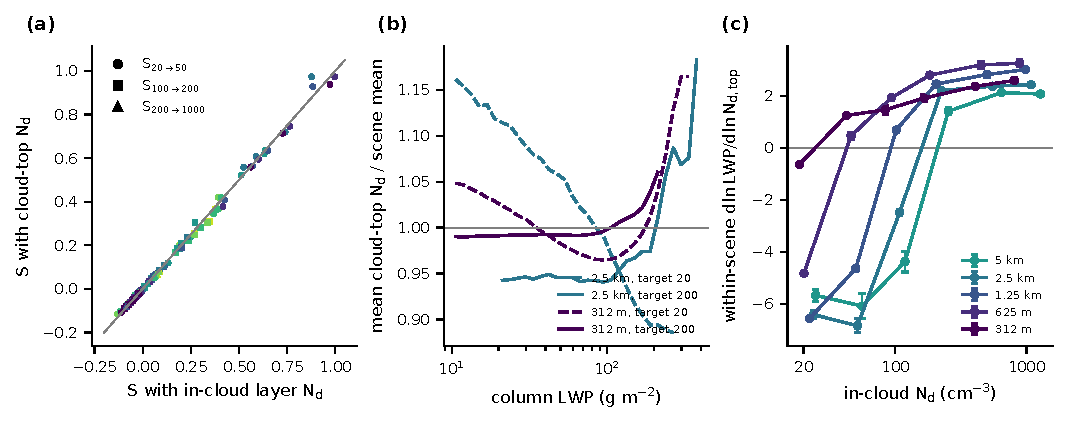
\includegraphics[width=\textwidth]{figures/fig11_cloudtop.pdf}
%DIFDELCMD < \caption{(a) Susceptibility computed with model-diagnosed cloud-top $\Nd$ against that computed with in-cloud layer $\Nd$ for all branches and configurations (3D turbulence off), coloured by grid spacing. (b) Mean cloud-top $\Nd$ relative to the scene mean as a function of column LWP, at 2.5\,km and 312\,m for target $\Nd$ of 20 and 200\,$\cmthree$ (hours 10--12). (c) Within-scene regression slope of column $\ln\LWP$ on column cloud-top $\ln\Nd$, with standard errors over the eight instants (suppression on, sedimentation factor 1, $\dx\leq5$\,km).}\label{fig:sat}
%DIFDELCMD < \end{figure}
%DIFDELCMD < 

%DIFDELCMD < %%%
%DIF < % ====================================================================
%DIFDELCMD < \section{Discussion}\label{sec:discussion}
%DIFDELCMD < %%%
%DIF < % ====================================================================
%DIFDELCMD < 

%DIFDELCMD < \subsection{Resolution dependence of the dominant adjustment pathway}
%DIFDELCMD < 

%DIFDELCMD < %%%
\DIFdel{At $\dx\geq10$\,km, where the simulations approximate single-column physics, entrainment in EAMxx is nearly insensitive to droplet sedimentation, the clouds are thick enough to precipitate substantially, and LWP increases monotonically with $\Nd$. This behaviour corresponds to the precipitation-suppression mechanism of \mbox{%DIFAUXCMD
\citet{albrecht1989}}\hskip0pt%DIFAUXCMD
. At finer grid spacing, entrainment increases ($\eta>1$), and the boundary layer warms, dries and deepens. The cloud thins and its base rises, so that rain production decreases and more of the rain evaporates below cloud. In addition, $\we$ becomes more sensitive to droplet sedimentation (Fig.~\ref{fig:entrain}a). Together these changes shift the LWP maximum from $\Nd\geq1000$ to about 100\,$\cmthree$. This picture is consistent with mixed-layer and LES arguments in which the turning point of the inverted-V relationship is set by the competition between precipitation and entrainment \mbox{%DIFAUXCMD
\citep{ackerman2004,wood2007,hoffmann2020,hoffmann2024}}\hskip0pt%DIFAUXCMD
. In EAMxx, the balance between these processes depends on horizontal grid spacing across the grey zone.
}%DIFDELCMD < 

%DIFDELCMD < %%%
\DIFdel{The extent to which this dependence reflects grey-zone physics rather than specific features of the configuration is not yet clear. Three model-specific factors co-vary with grid spacing in our experiment. SHOC's mixing length is capped at the grid spacing, and this cap is active throughout the boundary layer }\DIFdelend \DIFaddbegin \DIFadd{m levels, a capped mixing length and an entrainment efficiency of 2.0--2.6 }\DIFaddend at 312\,m\DIFdelbegin \DIFdel{. The physics time step and radiation interval decrease with grid spacing. The largest change in most quantities occurs between 10 and }\DIFdelend \DIFaddbegin \DIFadd{, are therefore unlikely to lie on a path towards the LES solution, and a converged answer probably requires entrainment to decrease again with vertical refinement. The grey zone for stratocumulus in EAMxx with SHOC begins at about }\DIFaddend 5\,km, \DIFdelbegin \DIFdel{where the resolved variance is still small and the circulations appear partly numerical. Any of these could contribute to the trends attributed above to grid spacing, and Sect.
~\ref{sec:limits} lists the experiments that would separate them.
}\DIFdelend \DIFaddbegin \DIFadd{and remedies would include scale-aware partitioning of turbulence \mbox{%DIFAUXCMD
\citep{boutle2014,efstathiou2015,honnert2011} }\hskip0pt%DIFAUXCMD
and vertical resolution at the inversion consistent with the horizontal grid \mbox{%DIFAUXCMD
\citep{bogenschutz2023rrm}}\hskip0pt%DIFAUXCMD
.
}\DIFaddend 

\DIFdelbegin \DIFdel{The weak negative branch at 312}\DIFdelend \DIFaddbegin \subsection{Relation to other models and to LES}

\DIFadd{The coarse configuration reproduces features of GCM behaviour, namely no cloud-cover response, light ubiquitous drizzle and a positive response driven by autoconversion, although with a 100}\DIFaddend \,\DIFdelbegin \DIFdel{m deserves particular caution. Its magnitude ($S\approx-0.04$ to $-0.05$) is an order of magnitude smaller than the steady-state adjustments inferred from LES of non-precipitating stratocumulus \mbox{%DIFAUXCMD
\citep{glassmeier2021} }\hskip0pt%DIFAUXCMD
and smaller than the observed slopes, which are themselves upper bounds \mbox{%DIFAUXCMD
\citep{gryspeerdt2019}}\hskip0pt%DIFAUXCMD
. Possible reasons include the transience of the runs, the absence of a droplet-size dependence of cloud-top evaporation in SHOC's saturation adjustment \mbox{%DIFAUXCMD
\citep{wang2003,hoffmann2019}}\hskip0pt%DIFAUXCMD
, the }\DIFdelend \DIFaddbegin \DIFadd{s time step and }\DIFaddend 50\,m \DIFdelbegin \DIFdel{vertical spacing at the inversion, and the humidity of the overlying air, which controls the strength of entrainment drying \mbox{%DIFAUXCMD
\citep{ackerman2004,chen2014}}\hskip0pt%DIFAUXCMD
; in our runs the $q_t$ jump at the inversion is 5.8--6.5\,g\,kg$^{-1}$. }%DIFDELCMD < 

%DIFDELCMD < \subsection{Relation to other models}
%DIFDELCMD < 

%DIFDELCMD < %%%
\DIFdel{The closest prior study is that of \mbox{%DIFAUXCMD
\citet{terai2020} }\hskip0pt%DIFAUXCMD
, who compared an ultra-parameterised multiscale model with }\DIFdelend \DIFaddbegin \DIFadd{levels it is not a GCM column. The comparison with \mbox{%DIFAUXCMD
\citet{mulmenstadt2024adj}}\hskip0pt%DIFAUXCMD
, who found an active sedimentation--entrainment coupling in E3SM single-column physics, indicates that whether this coupling appears in single-column physics depends on the turbulence scheme and its vertical representation of the inversion, which is pinned at a model level in our coarse runs. \mbox{%DIFAUXCMD
\citet{terai2020} }\hskip0pt%DIFAUXCMD
found weaker LWP increases at }\DIFaddend 250\,m \DIFdelbegin \DIFdel{cloud-resolving grids against a conventional multiscale model with }\DIFdelend \DIFaddbegin \DIFadd{than at }\DIFaddend 4\,km \DIFdelbegin \DIFdel{grids. They found a weaker LWP increase with aerosol at the finer resolution, caused by weaker LWP }\DIFdelend \DIFaddbegin \DIFadd{in a multiscale model because of weaker }\DIFaddend increases in non-raining clouds and a smaller raining fraction\DIFdelbegin \DIFdel{. Our results show }\DIFdelend \DIFaddbegin \DIFadd{, }\DIFaddend the same tendency \DIFdelbegin \DIFdel{for a single case in a doubly periodic configuration, in that the raining fraction and the precipitation-suppression term decrease with grid spacing, and LWP increases with $\Nd$ only weakly or not at all in the non-raining runsat sub-kilometre spacing}\DIFdelend \DIFaddbegin \DIFadd{as in our runs}\DIFaddend . \citet{sato2018} attributed \DIFdelbegin \DIFdel{the LWP decrease in their }\DIFdelend \DIFaddbegin \DIFadd{LWP decreases in a }\DIFaddend global cloud-system-resolving model to explicitly simulated condensation and evaporation\DIFdelbegin \DIFdel{responses to aerosol. That pathway is }\DIFdelend \DIFaddbegin \DIFadd{, a pathway }\DIFaddend absent from EAMxx\DIFdelbegin \DIFdel{, in which condensation is diagnosed by SHOC's saturation adjustment, so the mechanisms in the two models differ. }%DIFDELCMD < 

%DIFDELCMD < %%%
\DIFdel{The comparison with \mbox{%DIFAUXCMD
\citet{mulmenstadt2024adj} }\hskip0pt%DIFAUXCMD
is instructive. Using E3SM single-column physics, they found that switching sedimentation off removed the LWP decrease and that doubling it made the response more negative, and they concluded that GCM-type physics can represent the sedimentation--entrainment coupling. In our coarse runs, which use SHOC rather than the turbulence scheme of }\DIFdelend \DIFaddbegin \DIFadd{. The 312\,m polluted-branch value after 11\,h ($-0.04$) is of a similar magnitude to the weak nocturnal LWP decreases at high $\Nd$ in LES by \mbox{%DIFAUXCMD
\citet{hill2009} }\hskip0pt%DIFAUXCMD
and to the weak slopes expected for weakly and non-precipitating stratocumulus by \mbox{%DIFAUXCMD
\citet{hoffmann2025}}\hskip0pt%DIFAUXCMD
, and weaker than the LES ensemble of \mbox{%DIFAUXCMD
\citet{chen2025} }\hskip0pt%DIFAUXCMD
at a similar time after perturbation. Possible reasons include the absence of a size-dependent evaporation--entrainment effect in SHOC \mbox{%DIFAUXCMD
\citep{wang2003,hoffmann2019}}\hskip0pt%DIFAUXCMD
, }\DIFaddend the \DIFdelbegin \DIFdel{E3SM GCM, a }\DIFdelend 50\,\DIFdelbegin \DIFdel{m vertical grid and a 100\,s time step, entrainment is nearly insensitive to sedimentation, while the susceptibility with precipitation suppression on is sensitive to it through an interaction with autoconversion. The two results are not in conflict, because the configurations differ, but they show that the sedimentation--entrainment coupling in single-column physics depends on the turbulence scheme and its numerical settings. Our coarse runs are therefore not representative of GCM columns, which use much longer time steps, coarser vertical grids and different turbulence and microphysics schemes, and we do not draw conclusions about GCM behaviour from them. Likewise, GSRMs with other turbulence closures, such as Smagorinsky-type or scale-aware schemes that blend boundary-layer and LES closures \mbox{%DIFAUXCMD
\citep{boutle2014,efstathiou2015}}\hskip0pt%DIFAUXCMD
, may behave differently in the grey zone. Within EAMxx, the susceptibility at 2.5--5\,km (0.11--0.20 on the moderate branch, about 40--75\,\% of }\DIFdelend \DIFaddbegin \DIFadd{m levels, drizzle at the lower $\Nd$ levels, and }\DIFaddend the \DIFdelbegin \DIFdel{40}\DIFdelend \DIFaddbegin \DIFadd{moderately humid free troposphere of RF02 ($\Delta q_t$ of 5.8--6.5}\DIFaddend \,\DIFdelbegin \DIFdel{km value)lies between the values at 40}\DIFdelend \DIFaddbegin \DIFadd{g}\DIFaddend \,\DIFdelbegin \DIFdel{km and 312\,m. These results suggest that estimates of aerosol--cloud adjustments from GSRMs should be accompanied by resolution-sensitivity tests, and they motivate grey-zone-aware turbulence closures. The factorial approach also offers process-level targets, the precipitation-suppression term and the sensitivity to sedimentation, that could help to reduce equifinality in constraining aerosol--cloud parameterisations \mbox{%DIFAUXCMD
\citep{stanford2026}}\hskip0pt%DIFAUXCMD
}\DIFdelend \DIFaddbegin \DIFadd{kg$^{-1}$ at the inversion). Because solar heating buffers the nocturnal decline of LWP \mbox{%DIFAUXCMD
\citep{zhang2024,chen2024,sandu2008} }\hskip0pt%DIFAUXCMD
and the meteorological controls on albedo susceptibility differ between regions and times of day \mbox{%DIFAUXCMD
\citep{zhang2019,zhang2023}}\hskip0pt%DIFAUXCMD
, a diurnally averaged susceptibility cannot be inferred from these runs, and the nocturnal values are likely to overstate the thinning}\DIFaddend .

\DIFdelbegin %DIFDELCMD < \subsection{Relation to satellite-based estimates}
%DIFDELCMD < 

%DIFDELCMD < %%%
\DIFdel{Using model-diagnosed cloud-top $\Nd$ instead of layer-mean $\Nd$ changes $S$ by at most 0.1 in these simulations , but this does not test retrieval biases, and satellite analyses also use in-cloud LWP at pixel scale rather than domain means. The }\DIFdelend \DIFaddbegin \DIFadd{Satellite-style analyses of these simulations are hypothetical because the case is nocturnal; they are summarised in Appendix~\ref{app:sat}. With horizontally uniform CCN, }\DIFaddend within-scene \DIFdelbegin \DIFdel{covariation of LWP and }\DIFdelend \DIFaddbegin \DIFadd{variability accounts for less than 1\,\% of the variance of }\DIFaddend cloud-top \DIFaddbegin \DIFadd{$\ln\Nd$, so pooled composites reproduce the between-run slope, whereas a retrieval-like adiabatic }\DIFaddend $\Nd$ \DIFdelbegin \DIFdel{with uniform aerosol spans a range of slopes much wider than the susceptibilities and changes sign with grid spacing. This adds a model-based illustration to the concerns raised by \mbox{%DIFAUXCMD
\citet{ghan2016}}\hskip0pt%DIFAUXCMD
, \mbox{%DIFAUXCMD
\citet{gryspeerdt2019}}\hskip0pt%DIFAUXCMD
, \mbox{%DIFAUXCMD
\citet{arola2022} }\hskip0pt%DIFAUXCMD
and \mbox{%DIFAUXCMD
\citet{mahfouz2024} }\hskip0pt%DIFAUXCMD
that spatial co-variability is not a measure of the adjustment, and it cautions against evaluating the LWP adjustments of kilometre-scale models with satellite statistics that do not account for cloud-controlled $\Nd$ variability}\DIFdelend \DIFaddbegin \DIFadd{is about twice the model value and half of its variance is within-scene noise correlated with LWP, which lowers the pooled slope substantially. Selecting overcast, non-raining columns alone shifts the slope by up to 0.1. These results are consistent with \mbox{%DIFAUXCMD
\citet{gryspeerdt2019}}\hskip0pt%DIFAUXCMD
, \mbox{%DIFAUXCMD
\citet{quaas2020}}\hskip0pt%DIFAUXCMD
, \mbox{%DIFAUXCMD
\citet{arola2022}}\hskip0pt%DIFAUXCMD
, \mbox{%DIFAUXCMD
\citet{gryspeerdt2022amt} }\hskip0pt%DIFAUXCMD
and \mbox{%DIFAUXCMD
\citet{kokkola2025}}\hskip0pt%DIFAUXCMD
, and with large-domain LES analyses of satellite-style relationships \mbox{%DIFAUXCMD
\citep{costasuros2020,dipu2022}}\hskip0pt%DIFAUXCMD
, and they do not add a separate conclusion}\DIFaddend .

\DIFdelbegin %DIFDELCMD < \subsection{Limitations and required experiments}%%%
\DIFdelend \DIFaddbegin \subsection{Limitations and future experiments}\DIFaddend \label{sec:limits}

The study simulates \DIFdelbegin \DIFdel{a single }\DIFdelend \DIFaddbegin \DIFadd{one }\DIFaddend nocturnal, drizzling case with constant forcing\DIFdelbegin \DIFdel{and no shortwave radiation. The diurnal cycle modulates adjustments \mbox{%DIFAUXCMD
\citep{sandu2008}}\hskip0pt%DIFAUXCMD
, and the humidity above the inversion controls the sign of the entrainment response \mbox{%DIFAUXCMD
\citep{ackerman2004,chun2023}}\hskip0pt%DIFAUXCMD
. }\DIFdelend \DIFaddbegin \DIFadd{, and hours 10--12 have no counterpart in nature. }\DIFaddend Each configuration was run once \DIFdelbegin \DIFdel{. The quoted spread in $S$ reflects temporal sampling only, and the small negative susceptibilities at sub-kilometre spacing ($-0.02$ to $-0.09$) require confirmation with initial-condition ensembles of three to five members, for example at target $\Nd$ of 100, 200 and 1000\,$\cmthree$ at 2.5\,km and 312\,m}\DIFdelend \DIFaddbegin \DIFadd{with a common initial perturbation; the perturbed twins bound the internal noise but not the structural uncertainty}\DIFaddend . After 12\,h the sub-kilometre runs are still \DIFdelbegin \DIFdel{thinning by 4--6\,\%\,h$^{-1}$, and their susceptibilities have not levelled off, so a subset should be extended to 24\,h or longer \mbox{%DIFAUXCMD
\citep{glassmeier2021,bretherton2010}}\hskip0pt%DIFAUXCMD
.
}%DIFDELCMD < 

%DIFDELCMD < %%%
\DIFdel{The surface fluxes were prescribed. A bulk estimate that scales the latent heat flux with $q_\mathrm{s}(T_\mathrm{s})-q_t$ and the sensible heat flux with $T_\mathrm{s}-T_\mathrm{air}$, calibrated to the prescribed fluxes and the initial mixed layer with a sea surface temperature of 292\,K, suggests that interactive fluxes would have been 88--103 and 6--10\,W\,m$^{-2}$ at 312\,m instead of 93 and 16\,W\,m$^{-2}$, and 77--79 and 17--20\,W\,m$^{-2}$ at $\dx\geq10$\,km. The feedback would thus reduce the warming of the sub-kilometre boundary layers and would slightly increase their moisture supply, but at 312\,m the estimated latent heat flux remains below the entrainment drying of 105--131\,W\,m$^{-2}$. The estimate assumes fixed transfer coefficients and wind speed and should be tested with interactive surface fluxes over a fixed sea surface temperature. The absence of Coriolis force and wind nudging allowed the initial shear to decay, which may affect shear-driven entrainment in a resolution-dependent way.
}%DIFDELCMD < 

%DIFDELCMD < %%%
\DIFdel{The finest grid (312\,m, with physics columns 469\,m apart) is much coarser than the RF02 LES, and the vertical spacing at the inversion (about 50\,m) was held fixed. Neither LWP nor $\Shigh$ converged, so the results at 312\,m describe the trend of a grey-zone model and not a converged answer. A converged reference with the same microphysics, for example an LES with KK2000 autoconversion at the same $\Nd$ levels, is not available. The physics time step and radiation interval co-varied with grid spacing, and }\DIFdelend \DIFaddbegin \DIFadd{adjusting, and the steady-state values depend on exponential extrapolation. The vertical grid was fixed, }\DIFaddend SHOC's mixing length was capped at the grid spacing\DIFdelbegin \DIFdel{at 312\,m. Experiments with a common time step at 40, 5 }\DIFdelend \DIFaddbegin \DIFadd{, the time step co-varied with grid spacing, the radiation scheme lacks the above-inversion balancing term of the protocol, }\DIFaddend and \DIFdelbegin \DIFdel{2.5\,km, with a relaxed mixing-length cap at 625 and 312\,m, and with refined vertical spacing near the inversion would separate these effects from grid spacing. The decomposition of the susceptibility depends on the matching $\Nd$ of the suppression-off configuration and on an extrapolation to zero sedimentation. Simulations with $s=0$, with a second matching $\Nd$ (for example 200 or 1000\,$\cmthree$), or with a design in which the $\Nd$ seen by autoconversion and the $\Nd$ seen by sedimentation and radiation are varied independently, would give pivot-independent partial derivatives. The 240\,km domain contains 11--19 cells at sub-kilometre spacing, and at 5 and 2.5\,km the cell scale is probably limited by the effective resolution of the dynamical core. }%DIFDELCMD < 

%DIFDELCMD < %%%
\DIFdelend \DIFaddbegin \DIFadd{the absence of Coriolis force and wind nudging allowed the shear to decay. }\DIFaddend CCN were prescribed and \DIFdelbegin \DIFdel{horizontally }\DIFdelend uniform, without aerosol processing \DIFdelbegin \DIFdel{, scavenging or replenishment, which can matter for drizzle-driven transitions \mbox{%DIFAUXCMD
\citep{kazil2011,berner2013,goren2019,yamaguchi2017}}\hskip0pt%DIFAUXCMD
. Condensation and evaporation are computed by SHOC's }\DIFdelend \DIFaddbegin \DIFadd{\mbox{%DIFAUXCMD
\citep{kazil2011,berner2013,goren2019,yamaguchi2017}}\hskip0pt%DIFAUXCMD
, condensation was diagnosed by }\DIFaddend saturation adjustment, \DIFdelbegin \DIFdel{so the droplet-size dependence of cloud-top evaporation that contributes to the entrainment pathway in LES \mbox{%DIFAUXCMD
\citep{wang2003,bretherton2007,hoffmann2019} }\hskip0pt%DIFAUXCMD
is absent. Autoconversion follows }\DIFdelend \DIFaddbegin \DIFadd{and autoconversion followed }\DIFaddend KK2000 without \DIFdelbegin \DIFdel{a subgrid variance enhancement, so at coarse spacing it uses the mean in-cloud cloud water, whereas at fine spacing resolved variability partly provides such an enhancement; other autoconversion schemes would change the precipitation-suppression term \mbox{%DIFAUXCMD
\citep{morrison2020}}\hskip0pt%DIFAUXCMD
. Surface precipitation includes the flux of cloud droplets reaching the surface, which we estimate to be negligible except in }\DIFdelend \DIFaddbegin \DIFadd{subgrid enhancement. The decomposition into precipitation and sedimentation terms depends on the matching $\Nd$ of }\DIFaddend the \DIFdelbegin \DIFdel{coarse runs at target 20}\DIFdelend \DIFaddbegin \DIFadd{$\Nd$-independent configuration and on an extrapolation in $s$. The most informative future experiments would be a paired-perturbation design in which the runs are spun up at a common $\Nd$ and then perturbed and integrated for 24--36}\DIFaddend \,\DIFdelbegin \DIFdel{$\cmthree$ with $s=2$ and suppression off. Finally, because the P3 sedimentation diagnostics were not usable, the sedimentation flux at cloud top was not diagnosed, and the role of sedimentation was inferred from the sedimentation-factor experiments}\DIFdelend \DIFaddbegin \DIFadd{h with several seeds; a 312\,m pair with 10--15\,m levels near the inversion; a 36\,h set with a diurnal cycle; simulations with a sedimentation factor of zero and with a second matching $\Nd$ for the $\Nd$-independent configuration; tests with a common time step and a relaxed mixing-length cap; and an LES reference with the same microphysics}\DIFaddend .

%% ====================================================================
\conclusions\label{sec:conclusions}
%% ====================================================================

We analysed 288 doubly periodic EAMxx simulations of the \DIFaddbegin \DIFadd{nocturnal, drizzling }\DIFaddend DYCOMS-II RF02 \DIFdelbegin \DIFdel{drizzling stratocumulus with horizontal }\DIFdelend \DIFaddbegin \DIFadd{stratocumulus under constant forcing, with }\DIFaddend grid spacings from 40\,km to 312\,m, \DIFdelbegin \DIFdel{target }\DIFdelend \DIFaddbegin \DIFadd{six }\DIFaddend $\Nd$ \DIFdelbegin \DIFdel{from 20 to 1000\,$\cmthree$, three cloud-droplet sedimentation factors , and the $\Nd$ dependence of autoconversion switched on or off}\DIFdelend \DIFaddbegin \DIFadd{levels, three sedimentation factors and two autoconversion settings}\DIFaddend . Our conclusions are as follows.
\begin{enumerate}
\item \DIFdelbegin \DIFdel{The LWP response to $\Nd$ depends strongly on grid spacing. At 10--40}\DIFdelend \DIFaddbegin \DIFadd{After 10--12}\DIFaddend \,\DIFdelbegin \DIFdel{km LWP increased monotonically with $\Nd$ ($\Shigh=0.24$--0.27). With decreasing grid spacing the LWP maximum moved to lower $\Nd$, reaching about 100}\DIFdelend \DIFaddbegin \DIFadd{h, the moderate-branch LWP susceptibility decreased from 0.25 at 40}\DIFaddend \,\DIFdelbegin \DIFdel{$\cmthree$ }\DIFdelend \DIFaddbegin \DIFadd{km to $-0.05$ }\DIFaddend at 312\,m \DIFdelbegin \DIFdel{, where $\Shigh=-0.05$ and $\Svhigh=-0.04$ in single, still-evolving realisations.
}%DIFDELCMD < \item %%%
\item%DIFAUXCMD
\DIFdel{At coarse spacing, removing the $\Nd$ dependence of autoconversion removed the positive response, but the sensitivity to sedimentation interacted strongly with autoconversion, and the partition between the two depends on the matching $\Nd$ of the experiment design. With decreasing grid spacing, }\DIFdelend \DIFaddbegin \DIFadd{and }\DIFaddend the \DIFdelbegin \DIFdel{precipitation-suppression contribution on the moderate branch decreased from 0.34}\DIFdelend \DIFaddbegin \DIFadd{polluted branch became weakly negative at $\dx\leq2.5$\,km (23 of 24 configurations), whereas the clean-branch susceptibility increased from 0.37 to 0.62}\DIFaddend --0\DIFdelbegin \DIFdel{.39 to 0.04, and the gain in LWP from precipitation suppression at a diagnosed }\DIFdelend \DIFaddbegin \DIFadd{.75, largely through cloud cover. The optical-depth susceptibility stayed positive, so the implied brightening is reduced at high $\Nd$ and amplified at low }\DIFaddend $\Nd$ \DIFdelbegin \DIFdel{of 500\,$\cmthree$ decreased from 110 to 6\,$\gmm$}\DIFdelend \DIFaddbegin \DIFadd{at fine spacing}\DIFaddend .
\item \DIFdelbegin \DIFdel{At sub-kilometre spacing the weak decrease of LWP at high $\Nd$ was also present without the $\Nd$ dependence of autoconversion and became steeper with faster sedimentation on the polluted branch, consistent with a sedimentation--entrainment feedback. Its sign is not established, given its small magnitude, the transience of the runs and the absence of ensembles. }%DIFDELCMD < \item %%%
\item%DIFAUXCMD
\DIFdel{The ratio of entrainment warming to radiative cooling increased from about 0.5 at coarse spacing to 1.2--1.3 at }\DIFdelend \DIFaddbegin \DIFadd{The moderate-branch susceptibility tracks the ratio of surface precipitation to entrainment drying of the base state across grid spacings and sedimentation factors. In EAMxx, grid spacing acts mainly by setting the cloud regime through the entrainment rate, which determines cloud depth, cloud base, rain production and subcloud evaporation.
}\item \DIFadd{The resolution dependence develops over the run and the fine-grid runs are still adjusting. The }\DIFaddend 312\,m \DIFdelbegin \DIFdel{, entrainment drying exceeded the prescribed surface moisture supply, and the clouds thinned, lifted and produced less rain, most of which evaporated below cloud.
A mixed-layer budget associates the general thinning with this increase in entrainment , but it has little skill for the $\Nd$ dependence at $\dx\leq2.5$\,km.
}\DIFdelend \DIFaddbegin \DIFadd{moderate-branch value is well outside the internal noise and more likely to strengthen than to vanish at equilibrium, whereas the equilibrium sign of the polluted branch is undetermined.
}\DIFaddend \item \DIFdelbegin \DIFdel{Neither LWP nor its $\Nd$ response converged, and LWP decreased by 21--40}\DIFdelend \DIFaddbegin \DIFadd{Part of the increase of entrainment with refinement is implicit mixing at an inversion spanning two to three 50}\DIFaddend \,\DIFdelbegin \DIFdel{\% between 625 and 312}\DIFdelend \DIFaddbegin \DIFadd{m levels, the 5}\DIFaddend \,\DIFdelbegin \DIFdel{m at fixed diagnosed $\Nd$. SHOC's mixing length was capped by the grid spacing at }\DIFdelend \DIFaddbegin \DIFadd{km runs are dominated by near-grid-scale circulations, and the }\DIFaddend 312\,m \DIFdelbegin \DIFdel{, the time step co-varied with grid spacing, and 3D turbulence had a negligible effect. The 625\,m runs were closest to the RF02 observations at hours 4--6, but no grid spacing matched all observed quantities. }%DIFDELCMD < \item %%%
\item%DIFAUXCMD
\DIFdel{Susceptibilities computed with model-diagnosed cloud-top $\Nd$ agreed closely with those computed with layer $\Nd$, whereas within-scene LWP--$\Nd$ slopes with uniform aerosol ranged from $-7.9$ to $+3.4$ and changed sign with grid spacing.
}%DIFDELCMD < \end{enumerate}
%DIFDELCMD < %%%
\DIFdel{In EAMxx, the simulated LWP adjustment in drizzling stratocumulus thus depends on how the boundary-layer turbulence is partitioned between the grid and the turbulence scheme, as well as on the microphysics. Initial-condition ensembles, }\DIFdelend \DIFaddbegin \DIFadd{runs do not approximate LES. Extending these results to physical estimates requires vertical refinement at the inversion, }\DIFaddend longer and diurnally forced simulations, \DIFdelbegin \DIFdel{interactive surface fluxes, tests of time step and mixing-length limits, refined vertical grids, a second matching $\Nd$ for the suppression-off configuration and additional cases are needed to determine how far these results generalise.
}\DIFdelend \DIFaddbegin \DIFadd{and paired-perturbation ensembles.
}\end{enumerate}
\DIFaddend 

%% ====================================================================
\appendix
%% ====================================================================

\DIFdelbegin %DIFDELCMD < \section{Skill of the mixed-layer budget}\label{app:budget}
%DIFDELCMD < %%%
\DIFdelend \DIFaddbegin \section{Factorial decomposition}\label{app:decomp}
\DIFaddend 

\DIFdelbegin \DIFdel{Table~\ref{tab:skill} lists the skill of the mixed-layer budget for the LWP tendency at }\DIFdelend \DIFaddbegin \DIFadd{For }\DIFaddend each grid spacing \DIFdelbegin \DIFdel{, for the raw tendencies over all 2\,h windows from 2 to 12\,h and for the anomalies relative to the mean over the six }\DIFdelend \DIFaddbegin \DIFadd{and branch we fitted $S_\mathrm{dep}(s)=a_\mathrm{dep}+b_\mathrm{dep}s$ and $S_\mathrm{ind}(s)=a_\mathrm{ind}+b_\mathrm{ind}s$ for }\DIFaddend $\Nd$\DIFdelbegin \DIFdel{levels at fixed grid spacing, sedimentation factor, suppression setting and window.Figure~\ref{fig:budgetcheck} shows the anomalies. At 40, 20 }\DIFdelend \DIFaddbegin \DIFadd{-dependent }\DIFaddend and \DIFdelbegin \DIFdel{5\,km the budget reproduces both the tendencies and their }\DIFdelend $\Nd$\DIFdelbegin \DIFdel{dependence. At $\dx\leq2.5$}\DIFdelend \DIFaddbegin \DIFadd{-independent autoconversion over $s=0.5$, 1 and 2, and decomposed $S_\mathrm{dep}(1)=(a_\mathrm{dep}-a_\mathrm{ind})+b_\mathrm{ind}+(b_\mathrm{dep}-b_\mathrm{ind})+a_\mathrm{ind}$ into an autoconversion term at zero sedimentation, a sedimentation term, an interaction and a residual (Fig.~\ref{fig:decompA}, computed with the layer $\Nd$ of the first version). At $\dx\geq10$}\DIFaddend \,km the \DIFdelbegin \DIFdel{correlation for the anomalies in hours 10--12 is between $-0.02$ and 0.57, and the root-mean-square error is comparable to or larger than the standard deviation of the anomalies. The largest departures in the raw tendencies occur where the boundary layer is decoupled and cloud base departs from the mixed-layer lifting condensation level. Using the simulated $d\zb/dt$ instead of the estimate from the lifting condensation level degrades the agreement, because $\zb$ is quantised by the vertical grid}\DIFdelend \DIFaddbegin \DIFadd{autoconversion term on the moderate branch is 0.34--0.39 and the interaction $-0.07$ to $-0.08$, because $\Shigh$ decreases strongly with $s$ only with $\Nd$-dependent autoconversion; at finer spacing the autoconversion term decreases to 0.04--0.12. Because the $\Nd$-independent runs drizzle heavily at high $\Nd$, the extrapolation to $s=0$ has one residual degree of freedom and $S$ is convex in $s$ on the clean branch, the partition depends on the design and should not be read as a pivot-independent attribution. Section~\ref{sec:regime} offers a simpler interpretation, in which sedimentation moves the base state along the regime curve}\DIFaddend .

\DIFdelbegin %DIFDELCMD < \begin{table}[t]
%DIFDELCMD < \caption{Skill of the mixed-layer budget for $d\LWP/dt$ by grid spacing (3D turbulence off). $r$: correlation between budget and simulated tendency; RMSE and SD in $\gmm$\,h$^{-1}$. ``Raw'': all 2\,h windows (180 per grid spacing). ``Anomaly'': deviations from the mean over the six $\Nd$ levels at fixed grid spacing, sedimentation factor, suppression setting and window, for all windows and for hours 10--12.}\label{tab:skill}
%DIFDELCMD < \begin{tabular}{lrrrrrrr}
%DIFDELCMD < \tophline
%DIFDELCMD <  & \multicolumn{3}{c}{raw} & \multicolumn{1}{c}{anomaly, all} & \multicolumn{3}{c}{anomaly, hours 10--12} \\
%DIFDELCMD < $\dx$ & $r$ & RMSE & SD & $r$ & $r$ & RMSE & SD \\
%DIFDELCMD < \middlehline
%DIFDELCMD < 40\,km & 0.87 & 3.9 & 6.6 & 0.93 & 0.93 & 1.9 & 4.5 \\
20\,km & 0.83 & 4.0 & 6.4 & 0.91 & 0.87 & 2.3 & 3.6 \\
10\,km & 0.79 & 4.5 & 6.8 & 0.87 & 0.23 & 3.4 & 2.7 \\
5\,km & 0.90 & 5.1 & 11.2 & 0.89 & 0.85 & 3.0 & 5.8 \\
2.5\,km & 0.62 & 4.4 & 4.7 & 0.77 & -0.02 & 1.4 & 0.9 \\
1.25\,km & 0.38 & 4.8 & 4.9 & 0.57 & 0.08 & 1.4 & 0.9 \\
625\,m & 0.07 & 3.6 & 1.8 & 0.02 & 0.10 & 1.8 & 0.9 \\
312\,m & 0.44 & 2.7 & 2.2 & 0.51 & 0.57 & 0.8 & 0.8 \\
\bottomhline

%DIFDELCMD < \end{tabular}
%DIFDELCMD < \end{table}
%DIFDELCMD < %%%
\DIFdelend \DIFaddbegin \begin{figure}[t]
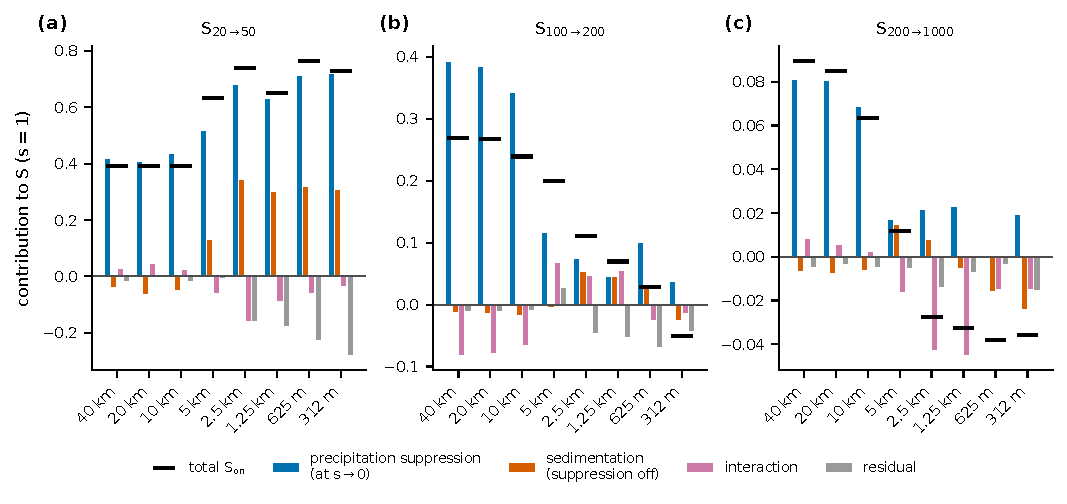
\includegraphics[width=\textwidth]{figures/figA1_decomposition.pdf}
\caption{Factorial decomposition of the susceptibility with $\Nd$-dependent autoconversion at sedimentation factor 1 (black bars) on the (a) clean, (b) moderate and (c) polluted branches.}\label{fig:decompA}
\end{figure}
\DIFaddend 

\DIFdelbegin %DIFDELCMD < \begin{figure}[t]
%DIFDELCMD < 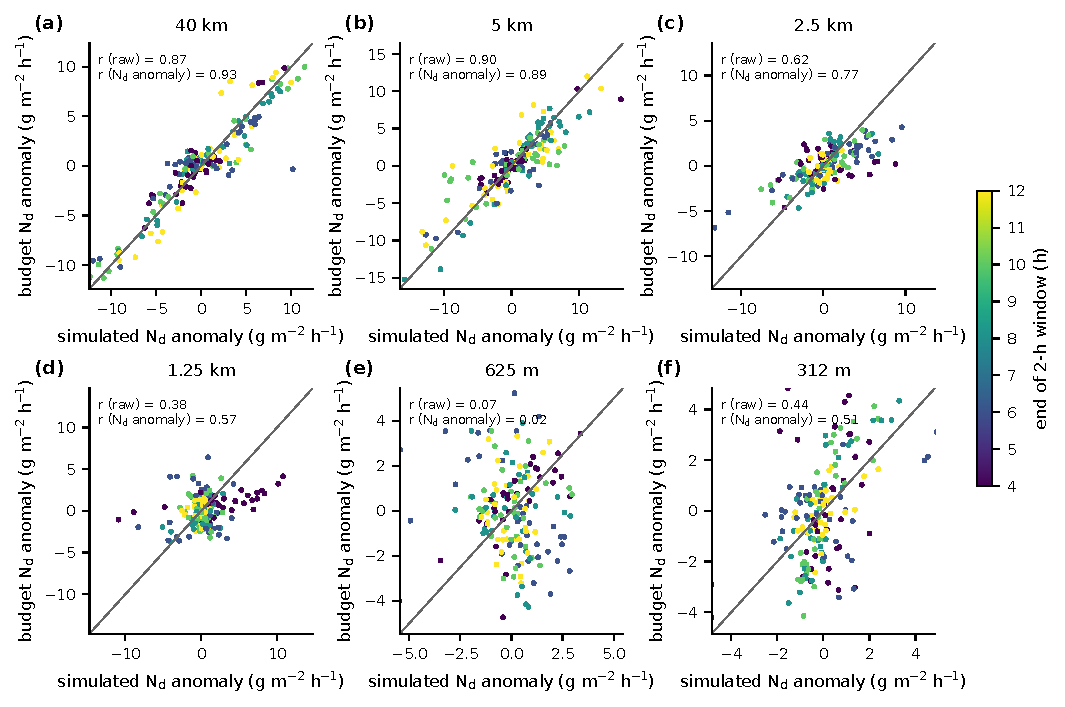
\includegraphics[width=\textwidth]{figures/figA1_budget_check.pdf}
%DIFDELCMD < \caption{Anomalies of $d\LWP/dt$ relative to the mean over the six $\Nd$ levels, from the mixed-layer budget against the simulated values, for all 2\,h windows (colour: end of window) at (a) 40\,km, (b) 5\,km, (c) 2.5\,km, (d) 1.25\,km, (e) 625\,m and (f) 312\,m. Each panel gives the correlation for the raw tendencies and for the anomalies.}\label{fig:budgetcheck}
%DIFDELCMD < \end{figure}
%DIFDELCMD < 

%DIFDELCMD < %%%
\DIFdelend \section{SHOC mixing length and activation floor}\label{app:shoc}

Figure~\ref{fig:shocmix}a shows the domain-mean SHOC mixing length \DIFdelbegin \DIFdel{in hours 10--12 }\DIFdelend at target 200\,$\cmthree$. At $\dx\geq10$\,km it reaches about 1600\,m \DIFdelbegin \DIFdel{in the upper boundary layer}\DIFdelend \DIFaddbegin \DIFadd{near 0.85\,$\zi$, about twice the boundary-layer depth, because the grid-length cap is not active}\DIFaddend . At 5\,km to 1.25\,km it peaks at 900--1100\,m \DIFdelbegin \DIFdel{near 0.85\,$\zi$ and is about }\DIFdelend \DIFaddbegin \DIFadd{and is }\DIFaddend 600--800\,m below. At 625\,m it is 480--610\,m, close to the cap\DIFdelbegin \DIFdel{of 625\,m}\DIFdelend , and at 312\,m it equals the cap \DIFdelbegin \DIFdel{of 312\,m }\DIFdelend nearly everywhere in the boundary layer. Figure~\ref{fig:shocmix}b shows \DIFaddbegin \DIFadd{that }\DIFaddend the in-cloud $\Nd$ \DIFdelbegin \DIFdel{profiles and }\DIFdelend \DIFaddbegin \DIFadd{follows }\DIFaddend the activation floor\DIFdelbegin \DIFdel{for target 200\,$\cmthree$. The in-cloud $\Nd$ follows the floor}\DIFdelend , which decreases with height\DIFdelbegin \DIFdel{because the prescribed CCN number does, so the diagnosed in-cloud $\Nd$ depends on the height of the cloud }\DIFdelend \DIFaddbegin \DIFadd{; between 6 and 12\,h the }\DIFaddend layer \DIFaddbegin \DIFadd{$\Nd$ decreases by about 3\,\%\,h$^{-1}$ at $\dx\leq625$\,m as the cloud rises into air with less CCN}\DIFaddend .

\DIFdelbegin %DIFDELCMD < \begin{figure}[t]
%DIFDELCMD < 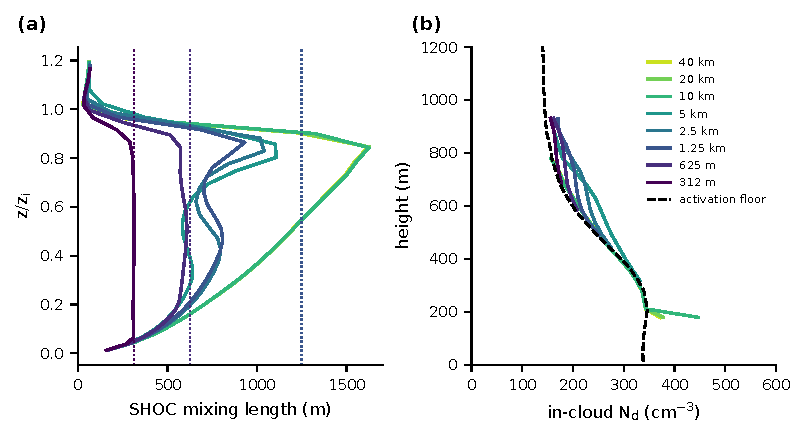
\includegraphics[width=0.75\textwidth]{figures/figA4_shocmix_nd.pdf}
%DIFDELCMD < \caption{(a) Domain-mean SHOC mixing length against $z/\zi$ and (b) in-cloud $\Nd$ (where the domain-mean liquid cloud fraction exceeds 0.2) with the activation floor (dashed), for target $\Nd=200\,\cmthree$, hours 10--12, suppression on and sedimentation factor 1. Dotted lines in (a) mark the grid-spacing cap at 1.25\,km, 625\,m and 312\,m.}\label{fig:shocmix}
%DIFDELCMD < \end{figure}
%DIFDELCMD < %%%
\DIFdelend \DIFaddbegin \begin{figure}[t]
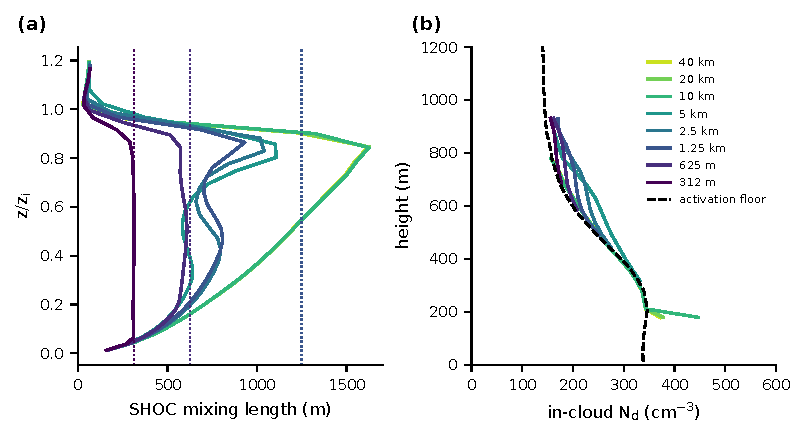
\includegraphics[width=0.75\textwidth]{figures/figA3_shocmix_nd.pdf}
\caption{(a) Domain-mean SHOC mixing length against $z/\zi$ and (b) in-cloud $\Nd$ with the activation floor (dashed), for target $\Nd=200\,\cmthree$, hours 10--12, $\Nd$-dependent autoconversion and sedimentation factor 1. Dotted lines in (a) mark the grid-spacing cap at 1.25\,km, 625\,m and 312\,m.}\label{fig:shocmix}
\end{figure}
\DIFaddend 

\DIFdelbegin %DIFDELCMD < \section{3D turbulence}%%%
\DIFdelend \DIFaddbegin \section{3D turbulence twins}\DIFaddend \label{app:t3d}

Figure~\ref{fig:t3d} shows the \DIFdelbegin \DIFdel{difference between }\DIFdelend \DIFaddbegin \DIFadd{differences between the 71 }\DIFaddend runs with 3D turbulence on and \DIFdelbegin \DIFdel{off for the 36 pairs at 625\,m and the 35 completed pairs at 312\,m}\DIFdelend \DIFaddbegin \DIFadd{their partners}\DIFaddend . LWP changes by between $-1.0$ and $+1.4\,\gmm$, cloud cover by between $-0.005$ and $+0.007$, and the entrainment rate by between $-0.13$ and $+0.02$\,mm\,s$^{-1}$\DIFdelbegin \DIFdel{. The only systematic signal is a slight reduction of entrainment.
These differences are an order of magnitude smaller than those between successive grid spacings or between $\Nd$ levels.
}\DIFdelend \DIFaddbegin \DIFadd{; the root-mean-square relative LWP difference in hours 10--12 is 0.6\,\%.
}\DIFaddend 

\DIFdelbegin %DIFDELCMD < \begin{figure}[t]
%DIFDELCMD < 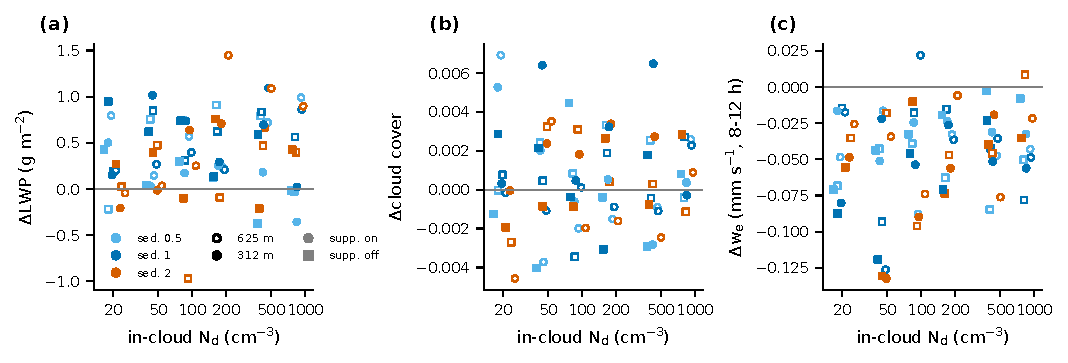
\includegraphics[width=\textwidth]{figures/figA2_turb3d.pdf}
%DIFDELCMD < \caption{Difference (3D turbulence on minus off) in (a) LWP, (b) cloud cover (LWP above 10\,$\gmm$) and (c) entrainment rate at 625\,m (open symbols) and 312\,m (filled symbols), coloured by sedimentation factor; circles: suppression on, squares: off.}\label{fig:t3d}
%DIFDELCMD < \end{figure}
%DIFDELCMD < %%%
\DIFdelend \DIFaddbegin \begin{figure}[t]
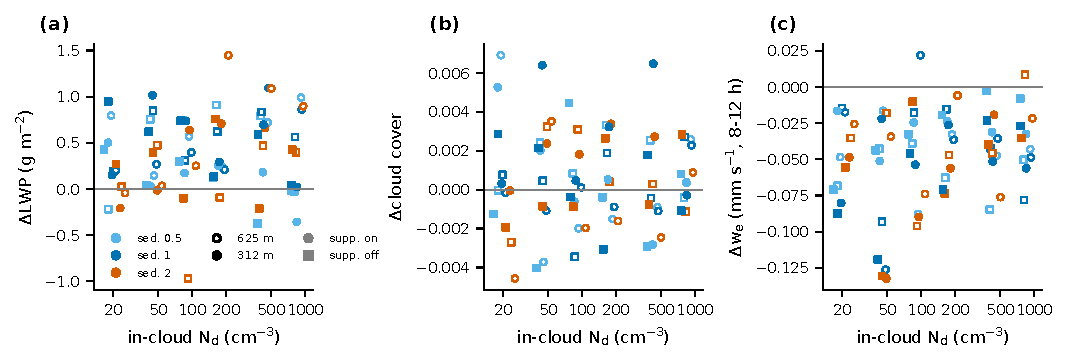
\includegraphics[width=\textwidth]{figures/figA4_turb3d.pdf}
\caption{Difference (3D turbulence on minus off) in (a) LWP, (b) cloud cover (LWP above 10\,$\gmm$) and (c) entrainment rate at 625\,m (open symbols) and 312\,m (filled symbols), coloured by sedimentation factor; circles: $\Nd$-dependent, squares: $\Nd$-independent autoconversion.}\label{fig:t3d}
\end{figure}
\DIFaddend 

\section{LWP spectra and distributions}\label{app:spectra}

\DIFdelbegin \DIFdel{Figure~\ref{fig:spectra} shows the LWP spectra and column-LWP distributions referred to in Sect.~\ref{sec:grey}. The spectral peak shifts from }\DIFdelend \DIFaddbegin \DIFadd{The LWP spectral peak (Fig.~\ref{fig:spectra}) lies at }\DIFaddend 48\,km at 5\,km \DIFdelbegin \DIFdel{to }\DIFdelend \DIFaddbegin \DIFadd{and }\DIFaddend about 30\,km at 2.5\,km\DIFdelbegin \DIFdel{and to }\DIFdelend \DIFaddbegin \DIFadd{, 6.4 and 8 physics-column spacings, which suggests that it is limited by the effective resolution of the dynamical core, and at }\DIFaddend 13--22\,km at 625 and 312\,m\DIFdelbegin \DIFdel{. The LWP distributions broaden and shift to lower values as the grid is refined, }\DIFdelend \DIFaddbegin \DIFadd{, an aspect ratio of 13--20 that is on the narrow side of observed closed cells \mbox{%DIFAUXCMD
\citep{wood2006,glassmeier2017}}\hskip0pt%DIFAUXCMD
. Pockets of open cells were observed during RF02 and in LES of the case \mbox{%DIFAUXCMD
\citep{stevens2005poc,savicjovcic2008}}\hskip0pt%DIFAUXCMD
, so the broken low-$\Nd$ fields are plausible, whereas the reduced cloud cover at high $\Nd$ at 312\,m has no observational counterpart in this case.
}

\begin{figure}[t]
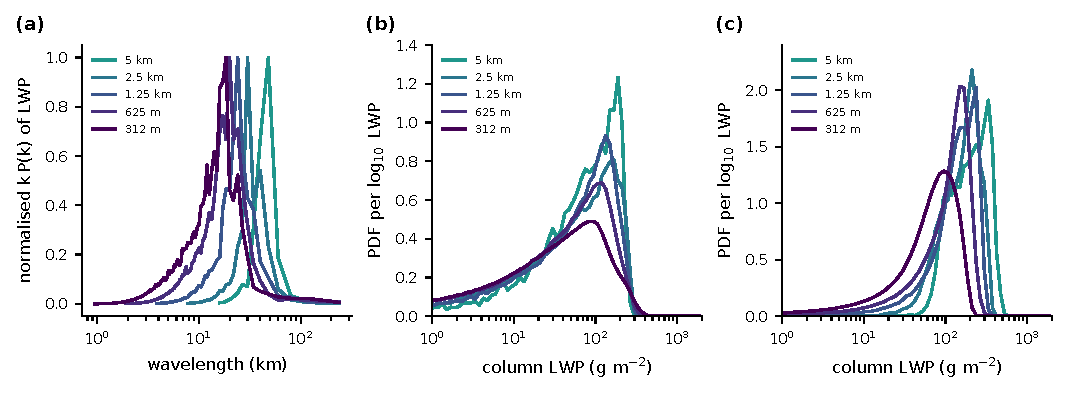
\includegraphics[width=\textwidth]{figures/figA5_spectra_pdf.pdf}
\caption{(a) Normalised radially averaged LWP spectra (hours 10--12) for target $\Nd=200\,\cmthree$. (b, c) Distributions of column LWP over hours 10--12 for target $\Nd$ of 20 and 1000\,$\cmthree$. $\Nd$-dependent autoconversion, sedimentation factor 1.}\label{fig:spectra}
\end{figure}

\section{Satellite-style analysis}\label{app:sat}

\DIFadd{To illustrate how satellite-style estimators would perform if these clouds could be observed, we pooled the cloudy columns of the six $\Nd$ runs at each grid spacing with equal weight per run and computed the regression of column $\ln\LWP$ on column $\ln\Nd$ (Fig.~\ref{fig:sat}). Columns were selected with a satellite-like filter: cloud-top liquid fraction above 0.9, LWP above 20\,$\gmm$, cloud-top effective radius below 15\,$\mu$m and optical depth above 3. The retrieval-like $\Nd$ follows the adiabatic formula of \mbox{%DIFAUXCMD
\citet{grosvenor2018} }\hskip0pt%DIFAUXCMD
applied to column LWP }\DIFaddend and \DIFaddbegin \DIFadd{cloud-top effective radius, at native resolution and after averaging to a common 3.75\,km scale \mbox{%DIFAUXCMD
\citep{mccomiskey2012}}\hskip0pt%DIFAUXCMD
. With model cloud-top $\Nd$, the within-scene share of the $\ln\Nd$ variance is below 1\,\% (within-scene standard deviation of $\ln\Nd$ at most 0.12, correlations between $-0.66$ and $+0.57$), so the pooled slope (0.10 at 312\,m to 0.27 }\DIFaddend at \DIFdelbegin \DIFdel{target $\Nd=20\,\cmthree$ they develop a large population of clear or nearly clear columns .
}\DIFdelend \DIFaddbegin \DIFadd{5\,km) equals the between-run slope; it exceeds the slope of in-cloud LWP for all columns (0.00 to 0.19) because the filter removes broken and drizzling columns. With retrieval-like $\Nd$, which is about twice the model value, the within-scene share is 46--52\,\% and the pooled slope (0.04--0.23) is only 25--50\,\% of the between-run slope (0.13--0.46), illustrating the dilution and bias by retrieval errors correlated with LWP \mbox{%DIFAUXCMD
\citep{jia2019,arola2022,kokkola2025,jia2022}}\hskip0pt%DIFAUXCMD
. Because activation in EAMxx does not depend on updraft speed, the model lacks the updraft-driven covariation of $\Nd$ and LWP found in nature, and the within-scene relationships should not be generalised to observations.
}\DIFaddend 

\DIFdelbegin %DIFDELCMD < \begin{figure}[t]
%DIFDELCMD < 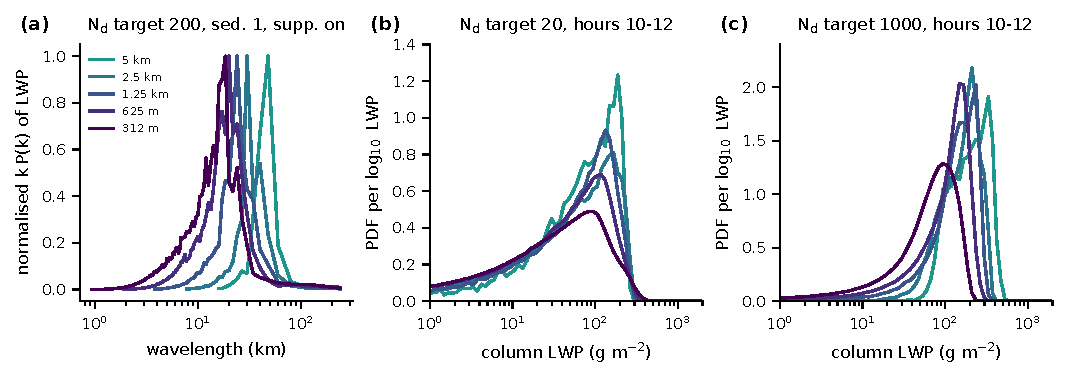
\includegraphics[width=\textwidth]{figures/figA3_spectra_pdf.pdf}
%DIFDELCMD < \caption{(a) Normalised radially averaged LWP spectra ($k\,P(k)$, hours 10--12) for target $\Nd=200\,\cmthree$. (b, c) Distributions of column LWP over hours 10--12 for target $\Nd$ of 20 and 1000\,$\cmthree$. Suppression on, sedimentation factor 1. In (b), clear columns at small LWP are off scale.}\label{fig:spectra}
%DIFDELCMD < \end{figure}
%DIFDELCMD < %%%
\DIFdelend \DIFaddbegin \begin{figure}[t]
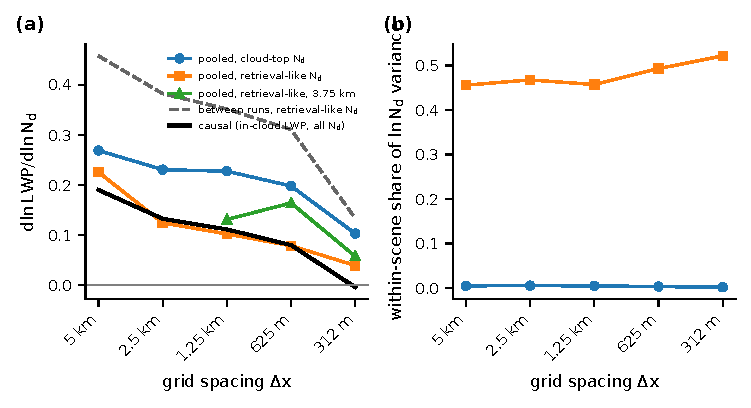
\includegraphics[width=0.7\textwidth]{figures/figA6_satellite.pdf}
\caption{(a) Pooled-composite slope of $\ln\LWP$ on $\ln\Nd$ for cloud-top $\Nd$ and retrieval-like $\Nd$ (native and 3.75\,km), the between-run slope with retrieval-like $\Nd$, and the slope of in-cloud LWP for all columns ($\Nd$-dependent autoconversion, sedimentation factor 1, hours 10--12). (b) Within-scene share of the pooled $\ln\Nd$ variance.}\label{fig:sat}
\end{figure}
\DIFaddend 

\noappendix

%% ====================================================================
\codedataavailability{\sloppy The model code is the E3SM branch \texttt{mahf708/eamxx/p3-cloud-sed-factor} at \url{https://github.com/mahf708/E3SM/tree/mahf708/eamxx/p3-cloud-sed-factor}, which contains E3SM pull request 9017 (the cloud-top output operator) and the P3 sedimentation-factor option. Run scripts and all analysis scripts used to produce the tables and figures are in the \texttt{sed-precsupp-study} directory of the branch \url{https://github.com/mahf708/scmlib/tree/sed-precsupp-study}. Model output and the derived tables are available from the corresponding contact on request.}

\authorcontribution{Naser Mahfouz and Johannes M\"ulmenst\"adt designed the experiments, and Naser Mahfouz implemented the model modifications and performed the simulations. The author, an AI system (Claude, Anthropic), designed and carried out the analysis and wrote the manuscript at the direction of Naser Mahfouz and Johannes M\"ulmenst\"adt. Human review of the manuscript is pending.}

\competinginterests{The author declares that there are no competing interests.}

\begin{acknowledgements}
Naser Mahfouz and Johannes M\"ulmenst\"adt (Pacific Northwest National Laboratory) designed and directed this study, and Naser Mahfouz is the contact person for correspondence. The simulations used the Energy Exascale Earth System Model (E3SM) and resources of the National Energy Research Scientific Computing Center (NERSC), a U.S. Department of Energy Office of Science User Facility, on the Perlmutter system. The analysis and the text were produced by an AI system (Claude, Anthropic); all analysis scripts are provided so that the results can be verified.
\end{acknowledgements}

\bibliographystyle{copernicus}
\bibliography{sedps_refs_diff}
 


\end{document}
